% Gelfand seminar notes, 1976-77: source pages P000659-P000706, P000752-P000758.
% English translation (AI-made, checked against the scans), cut page by page from the cumulative working reader A4-reader-chapters01-34-complete-first1527-separated-diplomatic-r35.
% \SourcePage{GELFAND-Pnnnnnn}{label} starts a scanned page; the second argument is the number written
% on the page, if any. Editorial notes give the page, a label and the transcriber's remark; \Unclear
% marks a doubtful reading.
\SourcePage{GELFAND-P000659}{unlabelled}
\underline{6/IX-76.}\quad \underline{Gelfand Sem.}

\underline{What should one know from physics?}\qquad [At right] (\underline{Following Sinai}?)
\Unclear{GELFAND-P000659}{sinai-attribution}{The note at right reads “Following Sinai?” with a question mark.}
\end{GelfandAdjacentEvidence}
\begin{GelfandAdjacentEvidence}{GELFAND-P000659}{2}


1. Classical mechanics and Ham. formalism.

\quad Arnold (\(\leq 30\) pp.), Landau and Lifshitz.

2. Quantum mechanics and scattering theory.

\quad Landau and Lifshitz, Quantum mechanics (minus the first two chapters).

\quad Fermi, Quantum mechanics.

3. Field theory and relativity.

\quad Landau and Lifshitz, Weinberg, Cosmology and the theory of gravitation (chapters 1–4).

4. Quantum field theory.

[crossed out]
\Incomplete{GELFAND-P000659}{cancelled-four}{The line under item 4 is heavily crossed out.}
\end{GelfandAdjacentEvidence}
\begin{GelfandAdjacentEvidence}{GELFAND-P000659}{3}


For next time, consult the physicists and type it up.

\underline{Quantum field theory}

1. Second quantization (Bose and Fermi). [Inserted below: statistics] --- Landau and Lifshitz.

2. Writing the equations [inserted in callout: of the field] using a functional integral,
\SourceFigure{GELFAND-P000659}{field-callout}{%
\par\smallskip
\begingroup\color{black}\GelfandFitDiagram{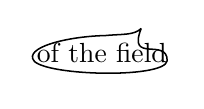
\begin{tikzpicture}[line width=.55pt]
\node at (0,0) {of the field};
\draw (.50,.31) .. controls (.32,-.14) and (.83,.20) .. (.83,-.10)
 .. controls (.80,-.34) and (-.85,-.29) .. (-.88,-.07)
 .. controls (-.92,.09) and (-.40,.21) .. (.05,.22)
 .. controls (.25,.24) and (.41,.22) .. (.50,.31);
\end{tikzpicture}}\endgroup\par
The callout after “equations” reads “поля” (of the field).}
\end{GelfandAdjacentEvidence}
\begin{GelfandAdjacentEvidence}{GELFAND-P000659}{4}

perturbation series, Feynman diagrams.

3. Renormalizations. --- Hepp.

4. Yang--Mills fields --- there are surveys.

\underline{Gindikin} (and Gelfand).
\underline{All about \(SL(2,\mathbb R)\).}
\[
G=SL(2,\mathbb R)
\]
\[
\begin{pmatrix}\alpha&\beta\\\gamma&\delta\end{pmatrix},
\qquad \det(\,)=1
\]
(hyperboloid in \(\mathbb R^4\))
\[
\alpha\delta-\beta\gamma=1
\]
It corresponds to a form with 2 pluses and 2 minuses:
\[
x^2+y^2-z^2-t^2=1.
\]
The group acts on the hyperboloid \(G\times G\) by left and right translations
\[
\underbrace{T_{(g_1,g_2)}g=g_1^{-1}gg_2}.
\]
\Unclear{GELFAND-P000659}{action-overwrite}{The final \(g_2\) is heavily retraced.}
\end{GelfandAdjacentEvidence}
\begin{GelfandAdjacentEvidence}{GELFAND-P000659}{5}


Any lin. transf. preserving the hyperboloid can be written in this form.

The stabilizer of the point \(e=\begin{pmatrix}1&0\\0&1\end{pmatrix}\)
consists of transfs. [crossed out]
\Incomplete{GELFAND-P000659}{cancelled-stabilizer}{A parenthesis is visible. Its contents are heavily crossed out.}
\end{GelfandAdjacentEvidence}

of the form \((g,g)\).


\Needspace{7\baselineskip}
\begin{GelfandAdjacentEvidence}{GELFAND-P000660}{1}
\SourcePage{GELFAND-P000660}{unlabelled}
[Line crossed out at top]
\Incomplete{GELFAND-P000660}{cancelled-top}{The line is heavily crossed out. Individual letter strokes remain visible.}
\end{GelfandAdjacentEvidence}
\begin{GelfandAdjacentEvidence}{GELFAND-P000660}{2}


\underline{Exercise:} compute the stabilizer subgrps. of other points.

Consider fns. on the hyperboloid.

For \(\beta\ne0\) convenient coordinates are [crossed out: \(\alpha,\beta,\delta\)]
\(\alpha,\delta,\beta\).
\Unclear{GELFAND-P000660}{coordinates}{The first sign of the crossed-out triple is retraced and the reading is tentative.}
\end{GelfandAdjacentEvidence}
\begin{GelfandAdjacentEvidence}{GELFAND-P000660}{3}


Fns. on the hyperboloid can be regarded as fns. \(\psi(\alpha,\delta,\beta)\).

The functions are to be integrated against the invariant measure:
\[
dg=\frac{d\alpha\,d\beta\,d\delta}{|\beta|}
\]
(inv. under motions of the hyperboloid).

We will consider the space \(\mathcal H=L^2(G)\) with respect to this measure.
\[
\|\psi\|^2=\int|\psi(g)|^2\,dg.
\]
\underline{Problem:} decompose the fns. into [circled and crossed out: irreducible]
subspaces inv. under
\Incomplete{GELFAND-P000660}{cancelled-irreducible}{The enclosed insertion above the line is crossed out.}
\end{GelfandAdjacentEvidence}
\begin{GelfandAdjacentEvidence}{GELFAND-P000660}{4}

\[
T_{(g_1,g_2)}\psi(g)=\psi(g_1^{-1}gg_2).
\]
In \(\mathbb R^4\) we consider hyperplanes
\[
\xi\alpha+\eta\delta-p\beta-q\gamma=\zeta.
\]
G. \underline{Philosophy:} divide into \underline{series} (an algebraic problem)

(Bernstein, Gelfand, Gelfand)
\Unclear{GELFAND-P000660}{three-credits}{The surname “Gelfand” is written twice in succession.}
\end{GelfandAdjacentEvidence}
\begin{GelfandAdjacentEvidence}{GELFAND-P000660}{5}


Series into representations --- a different (transcend.) problem.

This well-known example (Bargman, Gelfand and Graev, Molchanov, Strichartz, Vilenkin
et al.) --- everything about hyperboloids is already known.
\Unclear{GELFAND-P000660}{example-surname}{The first surname appears to be written “Bargman” in Latin script.}
\end{GelfandAdjacentEvidence}
\begin{GelfandAdjacentEvidence}{GELFAND-P000660}{6}


Into irreducibles --- \underline{no need}.

The following types of sections are possible.
\[
\text{I.}\quad \Delta=\begin{vmatrix}\xi&p\\q&\eta\end{vmatrix}<0
\quad\text{one-sheeted hyperboloid}\qquad 4\text{ parameters}
\]
\[
\text{II.}\quad \Delta=\begin{vmatrix}\xi&p\\q&\eta\end{vmatrix}>0
\]
\[
\left.
\begin{array}{rlrl}
\text{a)}&|\zeta|>2\sqrt{\Delta}&\text{one-sheeted hyperboloid}&4\\
\text{b)}&|\zeta|<2\sqrt{\Delta}&\text{two-sheeted hyperbol.}&4\\
\text{c)}&|\zeta|=2\sqrt{\Delta}&\text{cone}&3
\end{array}
\right\}\ \text{parameters}
\]
\Unclear{GELFAND-P000660}{sections-count}{The numbers 4, 4 and 3 are written at right and grouped with a brace.}
\end{GelfandAdjacentEvidence}
\begin{GelfandAdjacentEvidence}{GELFAND-P000660}{7}


\(\text{III.}\quad\Delta=0\) --- flat thing in hyperbol. cylinder\quad \(2\) parameters.
\SourceFigure{GELFAND-P000660}{degenerate-label}{%
\par\smallskip
\begingroup\color{black}\GelfandFitDiagram{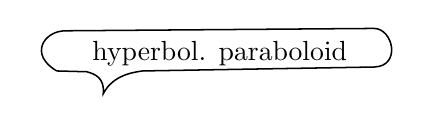
\begin{tikzpicture}[line width=.55pt]
\node at (0,.19) {hyperbol. paraboloid};
\draw (-2.07,-.03) .. controls (-2.43,.18) and (-2.23,.48) .. (-1.96,.48)
 -- (1.96,.51) .. controls (2.20,.51) and (2.31,.03) .. (1.96,.02)
 -- (-.98,-.03) .. controls (-1.21,-.06) and (-1.38,-.13) .. (-1.48,-.32)
 .. controls (-1.46,-.12) and (-1.58,-.07) .. (-1.69,-.04) -- (-2.07,-.03);
\end{tikzpicture}}\endgroup\par
“Hyperbol. paraboloid” is enclosed above the line. The single sign before “hyperbol. cylinder” resembles “в” (in).}
\end{GelfandAdjacentEvidence}



\Needspace{7\baselineskip}
\begin{GelfandAdjacentEvidence}{GELFAND-P000661}{1}
\SourcePage{GELFAND-P000661}{unlabelled}
\(A\) --- one-sheeted hyperboloid (\textit{cases} I, IIa), 4-param..

\(B\) --- two-sheeted hyperboloid (---»--- IIb), 4-param..

[Single letter crossed out: \(A\)?]
\Unclear{GELFAND-P000661}{cancel-letter}{The crossed-out letter between B and D resembles A.}
\end{GelfandAdjacentEvidence}
\begin{GelfandAdjacentEvidence}{GELFAND-P000661}{2}


\(D\) --- cones, 3-param..

\(E\) --- hyperbolic paraboloid (case III), 3-param..
\[
\psi\in\mathcal H.
\]
\[
\widehat\psi(\xi,\eta,p,q,\zeta)=
\int\psi(g)\delta(\xi\alpha+\eta\delta-p\beta-q\gamma-\zeta)\,dg.
\]
(Radon transform of the fn. in the whole space)

(G. The technique goes back to that of the 1947 paper by G. and Naimark.)

\(\mathcal H_A,\mathcal H_B,\mathcal H_D,\mathcal H_E\) --- fns. for which the integrals are 0
[sign crossed out: \(\varphi\)?] over the hyperplanes of the given family.
\Unclear{GELFAND-P000661}{overwritten-D}{The third subscript is overwritten. Its outline reads D.}
\end{GelfandAdjacentEvidence}
\begin{GelfandAdjacentEvidence}{GELFAND-P000661}{3}

\Unclear{GELFAND-P000661}{cancel-integrals}{A loop and a descending stroke in the crossed-out sign resemble φ.}
\end{GelfandAdjacentEvidence}
\begin{GelfandAdjacentEvidence}{GELFAND-P000661}{4}


[Crossed out: Problem [abbr.]?] How does one describe which fns. of 4 and 3 variables appear?
\Unclear{GELFAND-P000661}{cancel-question}{The crossed-out opening tentatively reads “Зад.” (Problem).}
\end{GelfandAdjacentEvidence}
\begin{GelfandAdjacentEvidence}{GELFAND-P000661}{5}


\underline{Main theorem 1.}

[Formula crossed out: \(\mathcal H=\mathcal H_A\ldots\)]
\Unclear{GELFAND-P000661}{cancel-decomp}{The crossed-out formula shows \(\mathcal H\), an equals sign and \(\mathcal H\) with subscript \(A\). The final sign is unclear.}
\end{GelfandAdjacentEvidence}
\begin{GelfandAdjacentEvidence}{GELFAND-P000661}{6}

\[
1.\quad \mathcal H=\mathcal H_A\overset{\circ}{+}\mathcal H_B.
\]
\Unclear{GELFAND-P000661}{sum-circle}{There is a small retraced circle above the plus sign.}
\end{GelfandAdjacentEvidence}
\begin{GelfandAdjacentEvidence}{GELFAND-P000661}{7}

\Unclear{GELFAND-P000661}{sum-mark}{A separate dot is also visible to the left of the plus sign.}
\end{GelfandAdjacentEvidence}
\begin{GelfandAdjacentEvidence}{GELFAND-P000661}{8}

\[
2.\quad \mathcal H_A=\mathcal H_D=\mathcal H_E.
\]
The fn. \(\widehat\psi\) satisfies a second-order ultrahyperbolic eq. that can be written down.

The families \(A,D,E\) are minimal.

Straight-line rulings --- a 3-param. family \(C\).
\Unclear{GELFAND-P000661}{ruling-adjective}{The abbreviation reads “Прямолин.” (straight-line).}
\end{GelfandAdjacentEvidence}
\begin{GelfandAdjacentEvidence}{GELFAND-P000661}{9}

\[
\begin{pmatrix}1&z\\0&1\end{pmatrix}
\quad\text{--- an example of a straight line},\qquad
\begin{pmatrix}h&z\\0&h^{-1}\end{pmatrix}
\quad(h\text{ --- fixed})
\]
or
\[
g_1^{-1}\begin{pmatrix}1&z\\0&1\end{pmatrix}g_2
\quad\text{(general form of a straight-line ruling)}.
\]
\Unclear{GELFAND-P000661}{ruling-repeat}{The same abbreviation for “straight-line” is repeated in parentheses.}
\end{GelfandAdjacentEvidence}
\begin{GelfandAdjacentEvidence}{GELFAND-P000661}{10}


\(C\) --- straight-line rulings.
\[
2'.\quad \mathcal H_A=\mathcal H_D=\mathcal H_E=\mathcal H_C.
\qquad\text{(discrete series)}
\]
\underline{Explicit specification of projectors and description of these spaces.}
\[
\alpha\delta-\beta\gamma=1.
\]
Consider the corresponding surface in \(\mathbb C^4\) with the same eq..
\Unclear{GELFAND-P000661}{last-referent}{The abbreviation before “in” reads “пов.” (surface).}
\end{GelfandAdjacentEvidence}
\begin{GelfandAdjacentEvidence}{GELFAND-P000661}{11}


and on it, the domains:
\Unclear{GELFAND-P000661}{last-pronoun}{The pronoun is “ней”, the feminine form used with “surface”.}
\end{GelfandAdjacentEvidence}



\Needspace{7\baselineskip}
\begin{GelfandAdjacentEvidence}{GELFAND-P000662}{1}
\SourcePage{GELFAND-P000662}{unlabelled}
\[
\begingroup\color{black}\GelfandFitDiagram{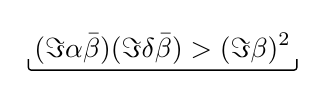
\begin{tikzpicture}[baseline=(inequality.base)]
\node[inner sep=2pt] (inequality)
  {$\displaystyle(\Im\alpha\bar\beta)(\Im\delta\bar\beta)>(\Im\beta)^2$};
\draw[line width=.5pt,rounded corners=1pt]
  ([yshift=4pt]inequality.south west) -- (inequality.south west) --
  (inequality.south east) -- ([yshift=4pt]inequality.south east);
\end{tikzpicture}}\endgroup
\qquad(1)
\]
Consider it in \(\mathbb C^3\).
\Unclear{GELFAND-P000662}{opening-pronoun}{The pronoun after “Consider” tentatively reads “её” (it).}
\end{GelfandAdjacentEvidence}
\begin{GelfandAdjacentEvidence}{GELFAND-P000662}{2}


It splits into 2 domains whose distinguished boundary is the real space \(\mathbb R^3\).

The inequality is inv. under fractional-linear transfs. (one of the Siegel domains).

Distinguished boundary \(G=SL(2,\mathbb R)\).

The domains are separated by the sign of the parentheses.

(The distinguished boundary of a domain \(D\) is the smallest set in \(\partial D\) such that a fn. holom. in \(D\) and cont. on \(\bar D\) is uniquely recovered from its restriction to that set.)

\underline{Lemma.} In \(\mathbb C^3\) with coords. \((\alpha,\beta,\delta)\)
[text crossed out] inequality (1) singles out 2 domains, each with distinguished boundary \(\mathbb R^3\).
\Incomplete{GELFAND-P000662}{cancel-lemma}{The short entry after the coordinate triple is heavily crossed out.}
\end{GelfandAdjacentEvidence}
\begin{GelfandAdjacentEvidence}{GELFAND-P000662}{3}

\Unclear{GELFAND-P000662}{lemma-continuation}{Before the 2 the writing tentatively reads “выд.” (singles out).}
\end{GelfandAdjacentEvidence}
\begin{GelfandAdjacentEvidence}{GELFAND-P000662}{4}


\underline{Theorem.} On the surface \(\alpha\delta-\beta\gamma=1\) in
\(\mathbb C^4\) there exist 2 domains inv. under real motions, with distinguished boundaries given by the hyperboloid
[sign crossed out] \(\alpha\delta-\beta\gamma=1\) in \(\mathbb R^4\).
\Incomplete{GELFAND-P000662}{cancel-theorem}{The initial sign to the left of the hyperboloid equation is crossed out.}
\end{GelfandAdjacentEvidence}
\begin{GelfandAdjacentEvidence}{GELFAND-P000662}{5}

Denote these domains by \(D_+\) and \(D_-\).

\underline{Main thm. 2.}
\[
\psi\in\mathcal H_A\ \Longleftrightarrow\ \psi=\psi_++\psi_-,\quad\text{where}
\]
\(\psi_+\) continues analyt. into \(D_+\), \(\psi_-\) continues analyt. into \(D_-\).

[Above the line: Denote [sign crossed out] the subspaces by
\(\mathcal H_{A,+}\) and \(\mathcal H_{A,-}\).]
\Incomplete{GELFAND-P000662}{subspace-insertion}{A sign with diverging strokes between “Denote” and “the subspaces” is crossed out.}
\end{GelfandAdjacentEvidence}
\begin{GelfandAdjacentEvidence}{GELFAND-P000662}{6}

\Unclear{GELFAND-P000662}{subspace-signs}{A thin vertical stroke crosses the long bar in the second subscript. The reading as a minus is tentative.}
\end{GelfandAdjacentEvidence}
\begin{GelfandAdjacentEvidence}{GELFAND-P000662}{7}


The projector onto \(\mathcal H_{A,+}\) is given by the fn.
\[
\int_G K(g_1,g_2)\psi(g_2)\,dg_2,
\]
where
\[
K(g_1,g_2)=c\,\frac{1}{[-\alpha_1\delta_2-\delta_1\alpha_2+\gamma_1\beta_2+\beta_1\gamma_2+2]^{3/2}}.
\]
\[
g_1=\begin{pmatrix}\alpha_1&\beta_1\\\gamma_1&\delta_1\end{pmatrix},
\qquad g_1\in D_+.
\]
The 2nd projector is analogous.
\[
\mathcal H_{A,+}\cap\mathcal H_{A,-}=\{0\},
\]
since [text crossed out] everything is in \(L^2\).
\Incomplete{GELFAND-P000662}{cancel-intersection}{The word after “since” is heavily crossed out.}
\end{GelfandAdjacentEvidence}
\begin{GelfandAdjacentEvidence}{GELFAND-P000662}{8}


\underline{\underline{The submerged part:}} Fourier-integral technique.

\(K(g_1,g_2)\) --- analogue of the Cauchy kernel.

\underline{Arnold’s conjecture.} \(D_+\) --- those that map the disc into itself,

\(D_-\) --- those that map the exterior of the disc [text crossed out] into itself,
\Incomplete{GELFAND-P000662}{cancel-circle}{A short entry after “disc” is heavily crossed out.}
\end{GelfandAdjacentEvidence}


\(SL(2,\mathbb R)\) --- preserves the circle.


\Needspace{7\baselineskip}
\begin{GelfandAdjacentEvidence}{GELFAND-P000663}{1}
\SourcePage{GELFAND-P000663}{unlabelled}
\underline{13/IX-76 }\quad\underline{Gelfand Sem..}

\underline{\underline{A.\,A. Kirillov.}}\quad\underline{Superalgebras, supergroups and supermanifolds.}

\underline{D.\,B. Fuchs.}\quad\underline{All about the Weil algebra.}

\(\mathfrak g\) --- Lie algebra. Construct from it the assoc. Weil algebra:
\[
W(\mathfrak g)
=\underset{\text{exterior algebra}}{\Lambda^*(\mathfrak g')}
 \underset{\mathrm{II}}{\otimes}
 \underset{\text{symmetric algebra}}{S^*(\mathfrak g')}.
\]
\Unclear{GELFAND-P000663}{notation-divider}{Two vertical strokes with shared crossbars appear below the tensor product sign.}
\end{GelfandAdjacentEvidence}
\begin{GelfandAdjacentEvidence}{GELFAND-P000663}{2}


If \(\mathfrak g\) has basis \(e_1,\ldots,e_n\), then the elements of \(W(\mathfrak g)\) ---
functions of 2\(n\) variables, super \(\mathfrak g\).
\SourceFigure{GELFAND-P000663}{hatched-lines}{%
\par\smallskip
\begingroup\color{black}\GelfandFitDiagram{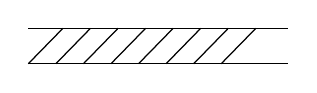
\begin{tikzpicture}[line width=.45pt]
  \draw (0,0) -- (3.3,0) (0,.45) -- (3.3,.45);
  \foreach \x in {0,.35,...,2.8}
    \draw (\x,0) -- ++(.44,.45);
\end{tikzpicture}}\endgroup\par
Diagonal strokes cross the two lines between the horizontal rules. The last entry tentatively reads “super” followed by a Fraktur g.}
\end{GelfandAdjacentEvidence}
\begin{GelfandAdjacentEvidence}{GELFAND-P000663}{3}


\underline{Grading:} \(\Lambda^p(\mathfrak g')\otimes S^q(\mathfrak g')\)
has degree \(p+2q\).

\underline{Differential:} \(d:W(\mathfrak g)\to W(\mathfrak g)\) with properties

1) \(d^2=0\), 2) acts in the usual way on [entry crossed out] the product.
\Incomplete{GELFAND-P000663}{cancel-product}{The short entry before “the product” is heavily crossed out.}
\end{GelfandAdjacentEvidence}
\begin{GelfandAdjacentEvidence}{GELFAND-P000663}{4}


Let \(h\in\underset{\substack{\Vert\\\Lambda^1(\mathfrak g')}}{\mathfrak g'}\).
Consider \(h\otimes1\in W(\mathfrak g)\).
\[
\begin{aligned}
d:\Lambda^1(\mathfrak g')\otimes S^0(\mathfrak g')\to{}&
\Lambda^2(\mathfrak g')\otimes S^0(\mathfrak g')\\
&\oplus\Lambda^0(\mathfrak g')\otimes S^1(\mathfrak g').
\end{aligned}
\]
\[
h\otimes1\ [h\text{? crossed out}]\ \mapsto
\bigl\{(g_1,g_2)\mapsto h([g_1,g_2])\bigr\}\otimes1;\qquad 1\otimes h.
\]
\Unclear{GELFAND-P000663}{cancel-map}{The crossed-out sign before the arrow resembles h.}
\end{GelfandAdjacentEvidence}
\begin{GelfandAdjacentEvidence}{GELFAND-P000663}{5}

This extends uniquely to a diff. with properties 1) and 2).

\underline{Property 2)}.
\[
\xi\in W^k(\mathfrak g),\quad\eta\in W^\ell(\mathfrak g)
\ \Longrightarrow\ d(\xi\cdot\eta)=d\xi\cdot\eta+(-1)^k\xi\cdot d\eta.
\]
On [entry crossed out] it is determined by the condition \(d^2=0\).
\Incomplete{GELFAND-P000663}{cancel-domain}{The entry after “On” is crossed out with diagonal strokes.}
\end{GelfandAdjacentEvidence}
\begin{GelfandAdjacentEvidence}{GELFAND-P000663}{6}

\SourceFigure{GELFAND-P000663}{domain-callout}{%
\par\smallskip
\begingroup\color{black}\GelfandFitDiagram{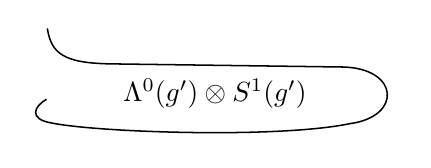
\begin{tikzpicture}[line width=.55pt]
\node at (0,0) {\(\Lambda^0(\mathfrak g')\otimes S^1(\mathfrak g')\)};
\draw (-2.13,.83) .. controls (-2.08,.51) and (-1.92,.39) .. (-1.33,.38)
  -- (1.63,.34) .. controls (2.34,.32) and (2.38,-.29) .. (1.71,-.38)
  .. controls (.78,-.57) and (-1.50,-.49) .. (-2.08,-.37)
  .. controls (-2.37,-.32) and (-2.30,-.16) .. (-2.14,-.07);
\end{tikzpicture}}\endgroup\par
The enclosed insertion is connected to the place after “On”.}
\end{GelfandAdjacentEvidence}
\begin{GelfandAdjacentEvidence}{GELFAND-P000663}{7}

\[
d:W^k(\mathfrak g)\to W^{k+1}(\mathfrak g).
\]
\[
d(h\otimes1)=(dh\otimes1)\oplus(1\otimes h),
\]
where \((dh)(g_1,g_2)\overset{\cdot}{=}h([g_1,g_2])\).

\(\overset{\cdot}{=}\) means \(\overset{\mathrm{def}}{=}\).
\[
(dh)(g_1,\ldots,g_{\ell+1})=
\]
\Unclear{GELFAND-P000663}{bottom-index}{The last sign in the subscript resembles \(1\), as in the exponent \(i+j-1\). The reading \(\ell+1\) is tentative.}
\end{GelfandAdjacentEvidence}
\begin{GelfandAdjacentEvidence}{GELFAND-P000663}{8}


[First sum crossed out: \(\sum(-1)^i h(\ldots)\).]
\Incomplete{GELFAND-P000663}{cancel-bottom}{The sum sign, the sign with superscript i, h, brackets and several instances of g are visible. The full entry cannot be read.}
\end{GelfandAdjacentEvidence}
\begin{GelfandAdjacentEvidence}{GELFAND-P000663}{9}

\[
\sum_{i<j}(-1)^{i+j-1}h([g_i,g_j],g_1,\ldots,\widehat g_i,\ldots,\widehat g_j).
\]
\Unclear{GELFAND-P000663}{bottom-arguments}{The first subscript after the commutator tentatively reads \(1\). The last two \(g\)s carry hats. An extra stroke is visible at the end.}
\end{GelfandAdjacentEvidence}



\Needspace{7\baselineskip}
\begin{GelfandAdjacentEvidence}{GELFAND-P000664}{1}
\SourcePage{GELFAND-P000664}{unlabelled}
\[
dh=\sum a_i h_{i_1}\wedge h_{i_2}
  =\sum a_i(h_{i_1}\otimes1)(h_{i_2}\otimes1).
\]
Differentiate by the Leibniz rule.

A nonzero element appears in \(\underline{\Lambda^1\otimes S^1}\).

Let \(e_1,\ldots,e_n\) --- a basis in \(\mathfrak g\), also a basis of linear fns. on \(\mathfrak g'\).

\(h^1,\ldots,h^n\) --- the dual basis in \(\mathfrak g'\).

Then
\[
\begingroup\color{black}\GelfandFitDiagram{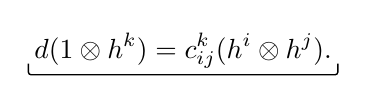
\begin{tikzpicture}[baseline=(structure.base)]
\node[inner sep=2pt] (structure)
  {$\displaystyle d(1\otimes h^k)=c_{ij}^k(h^i\otimes h^j).$};
\draw[line width=.5pt,rounded corners=1pt]
  ([yshift=4pt]structure.south west) -- (structure.south west) --
  (structure.south east) -- ([yshift=4pt]structure.south east);
\end{tikzpicture}}\endgroup
\]

\underline{Main theorem:} The homologies of the complex
\(\underline{\ldots}\to W^k\underline{\xrightarrow{d}}W^{k+1}\to\ldots\)
are equal to \(0\).

\underline{Next time:} how it works in char. classes.

\underline{A.\,A. Kirillov.} Devised to compute the homologies of simple compact Lie groups.

The easy part is the inv. forms.

Symmetric ones are easy to find. Skew-symmetric ones?

\(\omega^k\) --- a skew-symm. inv. diff. form.
\[
\omega^k\in\Lambda^k\otimes S^0+\ldots;\qquad d\omega^k=0.
\]
\Unclear{GELFAND-P000664}{omega-degree}{The superscript on \(\omega\) in the membership line is retraced. It tentatively reads \(k\), as in the nearby entries.}
\end{GelfandAdjacentEvidence}
\begin{GelfandAdjacentEvidence}{GELFAND-P000664}{2}

Then \(\omega^k\) --- the differential of a symm. expr..

Conclusion: as many skew-symm. [inserted above: inv.] of deg. \(k\) as symm. of deg. \(\frac{k+1}{2}\).
\SourceFigure{GELFAND-P000664}{invariant-callout}{%
\par\smallskip
\begingroup\color{black}\GelfandFitDiagram{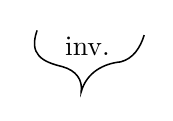
\begin{tikzpicture}[line width=.55pt]
\node at (0,.29) {inv.};
\draw (-.64,.49) .. controls (-.75,.18) and (-.57,.09) .. (-.32,.03)
  .. controls (-.14,-.02) and (-.06,-.14) .. (-.08,-.29)
  .. controls (-.01,-.04) and (.21,.07) .. (.42,.09)
  .. controls (.58,.13) and (.67,.27) .. (.72,.43);
\end{tikzpicture}}\endgroup\par
The abbreviation “inv.” is inserted above the line between “skew-symm.” and “deg.”.}
\end{GelfandAdjacentEvidence}
\begin{GelfandAdjacentEvidence}{GELFAND-P000664}{3}

\[
\text{---''---}\quad 3\qquad \text{---''---}\quad 2.
\]

\underline{Arnold.}\quad\underline{On works from the end of the last century on 2 questions.}

1) \(y''=F(x,y,y')\) (e.g., \(y''=0\)).

Tresse (a student of Sophus Lie) 1896, Acta Math. 1894.

\(y''=0\)\quad the graphs are straight lines.
\SourceFigure{GELFAND-P000664}{three-lines}{%
\par\smallskip
\begingroup\color{black}\GelfandFitDiagram{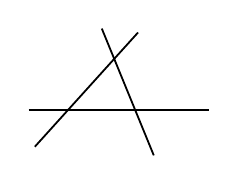
\begin{tikzpicture}[line width=.65pt]
\draw (-1.15,0)--(1.14,0);
\draw (-1.07,-.47)--(.24,.98);
\draw (-.22,1.03)--(.44,-.58);
\end{tikzpicture}}\endgroup\par
Three straight lines at right intersect pairwise to form a triangle.}
\end{GelfandAdjacentEvidence}
\begin{GelfandAdjacentEvidence}{GELFAND-P000664}{4}


There are configuration theorems (Pappus, Desargues, Pascal, etc.).

Can the solns. of the general eq. be straightened?

Linear menu \(\Longrightarrow\) all the config. thms. hold (Desargues for sinusoids).
\Unclear{GELFAND-P000664}{linear-phrase}{The second word tentatively reads “меню” (menu).}
\end{GelfandAdjacentEvidence}
\begin{GelfandAdjacentEvidence}{GELFAND-P000664}{5}

\Unclear{GELFAND-P000664}{desargues-phrase}{The word between “Desargues” and “sinusoids” tentatively reads “для” (for).}
\end{GelfandAdjacentEvidence}

\[
y''+a(x)y'+b(x)y=0
\]
is reduced by a diffeom. of the plane \((x,y)\), linear in \(y\):
\[
\begin{aligned}
x&=f(\tilde x)\\
y&=g(\tilde x)\tilde y
\end{aligned}
\]
Locally it is reduced to \(y''=0\).


\Needspace{7\baselineskip}
\begin{GelfandAdjacentEvidence}{GELFAND-P000665}{1}
\SourcePage{GELFAND-P000665}{unlabelled}
Consider an arbitrary family.

The infinitesimal theory is fairly well known.

\underline{E. Cartan} in 1924–25, --- projective connection ---

--- the solutions are geodesics with respect to this connection.

Projective connection --- a connection in a \(G\)-bundle, where \(G\) --- the projective group acting in the tangent space.

Space of line elements \((x,y,y')\).

2) In \(\mathbb R^3\) there are 2 direction fields.
\SourceFigure{GELFAND-P000665}{direction-grid}{%
\par\smallskip
\begingroup\color{black}\GelfandFitDiagram{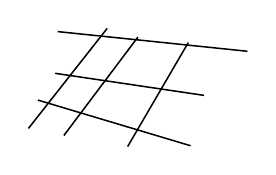
\begin{tikzpicture}[line width=.55pt]
  \draw (-.95,.48) -- (1.46,.23);
  \draw (-.98,-.05) -- (.91,-.33);
  \draw (-1.20,-.39) -- (.74,-.97);
  \draw (-1.32,-.75) -- (-.32,.52);
  \draw (-.87,-.84) -- (.07,.41);
  \draw (-.06,-.98) -- (.71,.34);
\end{tikzpicture}}\endgroup\par
Two families of three strokes each cross to form a slanted grid.}
\end{GelfandAdjacentEvidence}
\begin{GelfandAdjacentEvidence}{GELFAND-P000665}{2}


The diffeom. group of \(\mathbb R^3\) acts.

[retraced sign] To what form can one reduce it?
\Unclear{GELFAND-P000665}{question-prefix}{The isolated, heavily retraced sign before the question is undeciphered.}
\end{GelfandAdjacentEvidence}
\begin{GelfandAdjacentEvidence}{GELFAND-P000665}{3}


\underline{These problems are equivalent.}

Choose 1 dir., project along it onto the plane. There is a 2-param. family there, etc.
\Unclear{GELFAND-P000665}{restriction-word}{The abbreviation after “1 dir.” reads “спроект.” (project).}
\end{GelfandAdjacentEvidence}
\begin{GelfandAdjacentEvidence}{GELFAND-P000665}{4}


In his lifetime \underline{Blaschke} worked on it.
\Unclear{GELFAND-P000665}{blaschke-phrase}{The word before “Blaschke” tentatively reads “жизни” (life).}
\end{GelfandAdjacentEvidence}
\begin{GelfandAdjacentEvidence}{GELFAND-P000665}{5}


In \(\mathbb R^3\) there is a contact structure. (Planes spanned by tangent vectors).

The curves have locally the structure of a projective line.
\Unclear{GELFAND-P000665}{curve-word}{The abbreviation after “curves” tentatively reads “им.” (have).}
\end{GelfandAdjacentEvidence}
\begin{GelfandAdjacentEvidence}{GELFAND-P000665}{6}


(from the general theory of multidimensional bundles)
\Unclear{GELFAND-P000665}{bundle-adjective}{The adjective before “bundles” tentatively reads “многомерных” (multidimensional).}
\end{GelfandAdjacentEvidence}
\begin{GelfandAdjacentEvidence}{GELFAND-P000665}{7}


On the circle there are many inequivalent structures of a locally projective space.
\[
1)\quad\mathbb{RP}^1\qquad
2)\quad S^1\xrightarrow[\text{deg.}~2]{}\mathbb{RP}^1
\]
2) inequivalent structure.

\underline{Proof of inequivalence:} examine the vect. fields (infinitesim. automs. of this structure).
\Unclear{GELFAND-P000665}{proof-verb}{The abbreviation before “vect. fields” tentatively reads “просм.” (examine).}
\end{GelfandAdjacentEvidence}
\begin{GelfandAdjacentEvidence}{GELFAND-P000665}{8}

\[
\text{on }\mathbb{RP}^1\quad
\frac{\partial}{\partial x},\quad
x\frac{\partial}{\partial x},\quad x^2\frac{\partial}{\partial x}.
\]

\underline{Problem:} how [entry crossed out] the equation [entry crossed out] globally a locally projective space?
\Incomplete{GELFAND-P000665}{cancel-first}{The word between “how” and “the equation” is heavily crossed out.}
\end{GelfandAdjacentEvidence}
\begin{GelfandAdjacentEvidence}{GELFAND-P000665}{9}

\Incomplete{GELFAND-P000665}{cancel-second}{The word after “the equation” is crossed out with several strokes.}
\end{GelfandAdjacentEvidence}
\begin{GelfandAdjacentEvidence}{GELFAND-P000665}{10}

\Unclear{GELFAND-P000665}{question-word}{After the crossed-out word the writing reads “в целом локально” (globally, locally).}
\end{GelfandAdjacentEvidence}
\begin{GelfandAdjacentEvidence}{GELFAND-P000665}{11}


Take one soln. as a straight line.
\SourceFigure{GELFAND-P000665}{reference-line}{%
\par\smallskip
\begingroup\color{black}\GelfandFitDiagram{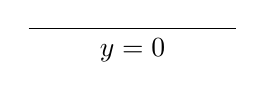
\begin{tikzpicture}[line width=.6pt]
\draw (-1.32,0)--(1.32,0);
\node[below] at (0,0) {\(y=0\)};
\end{tikzpicture}}\endgroup\par
The line at right is labelled \(y=0\).}
\end{GelfandAdjacentEvidence}
\begin{GelfandAdjacentEvidence}{GELFAND-P000665}{12}

\[
y''=a(x)y+b(x)p+\ldots
\]
[At right: terms of higher deg. in \(y'\).]
\Unclear{GELFAND-P000665}{margin-degree}{The first words of the note read “члены выс. степ.” (terms of higher deg.).}
\end{GelfandAdjacentEvidence}
\begin{GelfandAdjacentEvidence}{GELFAND-P000665}{13}

\[
p=y'.
\]

Straighten the lin. eq.. The coord. \(x\) is associated with points of its projective space.
\Unclear{GELFAND-P000665}{coordinate-line}{The abbreviation after “with” tentatively reads “т-ми” (points).}
\end{GelfandAdjacentEvidence}

\[
\begin{cases}
\tilde x=f(x),\\
\tilde y=g(x)y.
\end{cases}
\]
(\(f\) satisfies an eq. of Schwarz type).


\Needspace{7\baselineskip}
\begin{GelfandAdjacentEvidence}{GELFAND-P000666}{1}
\SourcePage{GELFAND-P000666}{unlabelled}
Hence a projective structure arises on \(\forall\) solns..

Now start with the quadr. part.
\[
y''=a(x)y^2+b(x)yy'+c(x)y'^2+\ldots
\]
\SourceFigure{GELFAND-P000666}{quadratic-marks}{%
\par\smallskip
\begingroup\color{black}\GelfandFitDiagram{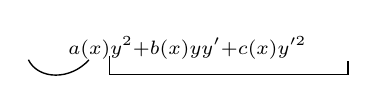
\begin{tikzpicture}[line width=.5pt]
\node at (0,0) {\(\scriptstyle a(x)y^2+b(x)yy'+c(x)y'^2\)};
\draw (-2.02,-.15) .. controls (-1.89,-.41) and (-1.48,-.41) .. (-1.25,-.15);
\draw (-.99,-.10) -- (-.99,-.34) -- (2.04,-.34) -- (2.04,-.16);
\end{tikzpicture}}\endgroup\par
An arc is drawn below the first term. A bracket runs under the next terms through \(c(x)y'^2\).}
\end{GelfandAdjacentEvidence}
\begin{GelfandAdjacentEvidence}{GELFAND-P000666}{2}


Now diffeom. of the plane of the form:
\[
\begin{cases}
\tilde x=x+yf(x,y),\\
\tilde y=y(1+yg(x,y)).
\end{cases}
\]
Kill \(b\) and \(c\) with these diffeom..

There remains \(a\), determined up to a mult. constant.
\[
\underline{\underline{a(x)(dx)^{5/2}}}\qquad\text{determined up to a mult. constant.}
\]
This is a 5/2-form along the solution, determined up to a mult. const. depending on the solution.

\underline{Theorem.} If \(a(x)(dx)^{5/2}\equiv0\), \underline{then the eq. can be straightened}.

(in formal series)

Further diffeoms. lead to \(\underline{\underline{y''=y'^2A(x,y,y')}}\).

Consider an eq. of the form \(\underline{y''=P_3(y')}\) --- a 3rd-degree poly. in \(y'\).

This class is inv. under diffeomorphisms.

The occurrence of these eqs. was discovered by \underline{R. Liouville}.
\Unclear{GELFAND-P000666}{liouville-verb}{The verb before the name tentatively reads “открыл” (discovered).}
\end{GelfandAdjacentEvidence}
\begin{GelfandAdjacentEvidence}{GELFAND-P000666}{3}


\underline{Scalar invariant.}

From this, a form of \(\forall\) other degs. (in partic. a vect. field).
\[
\begingroup\color{black}\GelfandFitDiagram{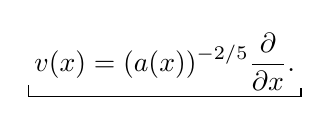
\begin{tikzpicture}[baseline=(field.base)]
\node[inner sep=2pt] (field)
  {$\displaystyle v(x)=(a(x))^{-2/5}\frac{\partial}{\partial x}.$};
\draw[line width=.5pt] ([yshift=4pt]field.south west) -- (field.south west) --
  (field.south east) -- ([yshift=3pt]field.south east);
\end{tikzpicture}}\endgroup
\]
\Unclear{GELFAND-P000666}{from-this}{The opening tentatively reads “Из эт.” (from this).}
\end{GelfandAdjacentEvidence}
\begin{GelfandAdjacentEvidence}{GELFAND-P000666}{4}


\underline{Now construct a scalar:} we want it to commute with the action of the projective group.
\Unclear{GELFAND-P000666}{scalar-clause}{After “we want” the entry reads “чтобы коммутир.” (to commute).}
\end{GelfandAdjacentEvidence}

We obtain invariants:

\(I_2,I_3,\ldots\) --- invariants.

Consider the 2-jet of the field. On 2-jets the projective group acts by the adjoint representation.
\[
\begin{gathered}
\underline{I_2=2v''v-v'^2}\\
\underline{I_3=vI_2'}\\
\text{---\quad ---\quad ---}\\
\underline{I_n=vI_{n-1}'}
\end{gathered}
\]
\underline{Gelfand conjecture:} connected with Gelfand–Fuchs cohomology.

\underline{Pommaret} worked on diff. invariants.


\Needspace{7\baselineskip}
\begin{GelfandAdjacentEvidence}{GELFAND-P000667}{1}
\SourcePage{GELFAND-P000667}{unlabelled}
\underline{20/IX-76 }\quad\underline{Gelfand Sem..}

\underline{S.\,P. Novikov.}\quad\underline{Superalgebras in physics.}

[Crossed out: Rev.?] \underline{Ogievetsky’s review in UFN and Zumino’s review}.
\Unclear{GELFAND-P000667}{cancel-review}{The crossed-out opening tentatively reads “Обз.” (Rev.).}
\end{GelfandAdjacentEvidence}
\begin{GelfandAdjacentEvidence}{GELFAND-P000667}{2}

\SourceFigure{GELFAND-P000667}{margin-authors}{%
\par\smallskip
\begingroup\color{black}\GelfandFitDiagram{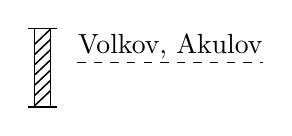
\begin{tikzpicture}[line width=.55pt]
  \draw (-.10,0) rectangle (.10,1.00);
  \draw (-.18,0) -- (.18,0) (-.18,1.00) -- (.18,1.00);
  \foreach \y in {.02,.15,...,.80}
    \draw (-.10,\y) -- ++(.20,.19);
  \node[anchor=west,inner sep=0] (names) at (.44,.77) {Volkov, Akulov};
  \draw[dashed] ([yshift=-1pt]names.south west) -- ([yshift=-1pt]names.south east);
\end{tikzpicture}}\endgroup\par
The surnames are underlined with broken strokes in the right margin. A narrow hatched mark stands to their left.}
\end{GelfandAdjacentEvidence}
\begin{GelfandAdjacentEvidence}{GELFAND-P000667}{3}


Superalgebra [Crossed out: Lie?] --- a direct sum
\(L=L_{\text{even}}\oplus L_{\text{odd}}=L_0\oplus L_1\).
\Unclear{GELFAND-P000667}{cancel-super}{The strokes of the short crossed-out word resemble “Ли” (Lie).}
\end{GelfandAdjacentEvidence}
\begin{GelfandAdjacentEvidence}{GELFAND-P000667}{4}


\([a,b]\) defines the struct. of a graded Lie algebra.
\[
[a,b]=(-1)^{da\cdot db+1}[b,a],\qquad da=\dim a.
\]
\Unclear{GELFAND-P000667}{degree-notation}{The definition of \(da\) reads “dim a”.}
\end{GelfandAdjacentEvidence}


The Jacobi id. also holds with signs.

Let \(L_0\) and \(L_1\) be embedded in an assoc. algebra (e.g., of matrices).

\(L\) --- a subalgebra of the matrix alg., closed under the operation
\[
\begin{aligned}
1)\quad &a,b\in L_0\ \Longrightarrow\ ab-ba=[a,b]\in L_0,\\
2)\quad &a,b\in L_1\ \Longrightarrow\ ab+ba=[a,b]\in L_0.
\end{aligned}
\]


\Needspace{7\baselineskip}
\begin{GelfandAdjacentEvidence}{GELFAND-P000668}{1}
\SourcePage{GELFAND-P000668}{unlabelled}
\[
3)\quad a\in L_0,\ b\in L_1\ \Longrightarrow\ ab-ba=[a,b]\subset L_1.
\]
Or
\[
\begin{gathered}
[a,b]=(-1)^{\varepsilon_1\varepsilon_2+1}[b,a],\\
\varepsilon_1=\operatorname{deg} a,\qquad
\varepsilon_2=\operatorname{deg} b.
\end{gathered}
\]
Concrete superalgebras were first considered in the work of Gelfand and Likhtman.
\[
\mu=0,1,2,3.
\]
Everything in \(\mathbb R^4\) Minkowski.
\[
\eta_{\nu,\mu}=\begin{pmatrix}
-1&&&0\\ &1&&\\ &&1&\\0&&&1
\end{pmatrix}\quad\text{--- metric.}
\]
\underline{space of spinors} --- 4-dimensional space
[inserted above: real. Word crossed out.] (with basis) \(Q_j\), \(j=1,2,3,4\).
\SourceFigure{GELFAND-P000668}{cancel-complex}{%
\par\smallskip
\begingroup\color{black}\GelfandFitDiagram{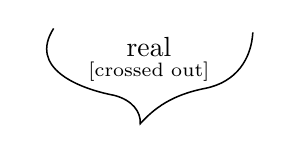
\begin{tikzpicture}[line width=.55pt]
\node at (0,.30) {real};
\node at (0,-.02) {\scriptsize [crossed out]};
\draw (-1.21,.53) .. controls (-1.53,.03) and (-.91,-.23) .. (-.44,-.32)
  .. controls (-.21,-.38) and (-.10,-.53) .. (-.11,-.68)
  .. controls (.07,-.48) and (.30,-.31) .. (.72,-.23)
  .. controls (1.11,-.15) and (1.30,.14) .. (1.32,.48);
\end{tikzpicture}}\endgroup\par
“Real” is written in the enclosed insertion. The lower word is crossed out.}
\end{GelfandAdjacentEvidence}
\begin{GelfandAdjacentEvidence}{GELFAND-P000668}{2}

\SourceFigure{GELFAND-P000668}{basis-callout}{%
\par\smallskip
\begingroup\color{black}\GelfandFitDiagram{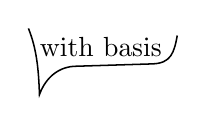
\begin{tikzpicture}[line width=.55pt]
\node at (.09,.25) {with basis};
\draw (-.83,.49) .. controls (-.72,.22) and (-.70,-.06) .. (-.69,-.35)
  .. controls (-.61,-.13) and (-.44,.01) .. (-.22,.01)
  -- (.75,.04) .. controls (.98,.05) and (1.02,.18) .. (1.06,.40);
\end{tikzpicture}}\endgroup\par
The second outlined insertion, “with basis”, points to the start of the list.}
\end{GelfandAdjacentEvidence}
\begin{GelfandAdjacentEvidence}{GELFAND-P000668}{3}

\[
\alpha=\sum\alpha^j Q_j.
\]
Matrix algebra generated by matrices \(\gamma_\mu\) (real) --- Majorana basis.
\[
\gamma_\mu\gamma_\nu+\gamma_\nu\gamma_\mu=2\eta_{\nu\mu}.
\qquad(\approx\text{ quaternions})
\]
Choose 4 matrices \(\gamma_\mu\), real and forming a Majorana basis

(see Akhiezer, Berestetskii).

Set
\[
\begin{aligned}
\bar Q_j&=Q_j\gamma_0;\\
\bar\alpha&=\alpha\gamma_0.
\end{aligned}
\]
\Unclear{GELFAND-P000668}{spinor-letter}{The letter \(Q\) has a descending diagonal stroke.}
\end{GelfandAdjacentEvidence}
\begin{GelfandAdjacentEvidence}{GELFAND-P000668}{4}


\(L_0\) --- alg. of [crossed out: Poincaré] translations.
\Unclear{GELFAND-P000668}{poincare-cancel}{“Poincaré” is crossed out before “translations”.}
\end{GelfandAdjacentEvidence}
\begin{GelfandAdjacentEvidence}{GELFAND-P000668}{5}


\(L_1\) --- space of spinors.
\[
\begin{aligned}
1)\quad &[L_1,L_0]=0,\\
2)\quad &[L_1,L_1]\text{ --- ?}
\end{aligned}
\]
\[
[\bar Q_i,\bar Q_j]=-2(\gamma^\mu)_{ij}P_\mu.
\]
\(P_\mu\) --- Poincaré translation oper., \(\mu\) --- index.

G. \underline{Problem.} extend the Poincaré alg. to a superalgebra.

\SourceFigure{GELFAND-P000668}{field-figure}{%
\par\smallskip
\begingroup\color{black}\GelfandFitDiagram{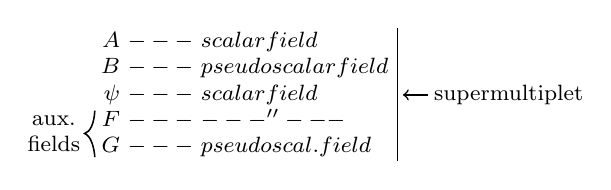
\begin{tikzpicture}[line width=.55pt, every node/.style={font=\footnotesize}]
\node[anchor=west,inner sep=0] (fields) at (.86,0) {%
  \(\begin{array}{@{}r@{\ \text{---}\ }l@{}}
  A & \text{scalar field}\\
  B & \text{pseudoscalar field}\\
  \psi & \text{scalar field}\\
  F & \text{---''---}\\
  G & \text{pseudoscal. field}
  \end{array}\)};
\draw (.79,-.20) .. controls (.78,-.37) and (.73,-.47) .. (.66,-.49)
  .. controls (.74,-.52) and (.78,-.66) .. (.79,-.79);
\node[align=center,inner sep=0] at (.27,-.49) {aux.\\fields};
\draw ([xshift=3pt]fields.north east) -- ([xshift=3pt]fields.south east);
\draw[<-] ([xshift=5pt]fields.east) -- ([xshift=14pt]fields.east);
\node[anchor=west,inner sep=0] at ([xshift=16pt]fields.east) {supermultiplet};
\end{tikzpicture}}\endgroup\par
The brace at left groups \(F,G\). The label at right points to the vertical line beside the list.}
\end{GelfandAdjacentEvidence}
\begin{GelfandAdjacentEvidence}{GELFAND-P000668}{6}

\Unclear{GELFAND-P000668}{field-label}{The label beside \(\psi\) also reads “скал. поле” (scalar field).}
\end{GelfandAdjacentEvidence}
\begin{GelfandAdjacentEvidence}{GELFAND-P000668}{7}

\[
\begin{aligned}
L={}&-\tfrac12\bigl((\partial_\nu A)^2+(\partial_\mu B)^2
+i\bar\psi\gamma^\mu\partial_\mu\psi\\
&\qquad +m^2A^2+m^2B^2+im\bar\psi\psi\bigr)\\
&+gmA(A^2+B^2)-g_2^2(A^2+B^2)^2\\
&-ig\,[im\text{? crossed out}]\,\bar\psi(A-\gamma_5B)\psi.
\end{aligned}
\]
\Unclear{GELFAND-P000668}{kinetic}{Faint strokes before the raised \(\mu\) after \(\bar\psi\) tentatively read \(\gamma\).}
\end{GelfandAdjacentEvidence}
\begin{GelfandAdjacentEvidence}{GELFAND-P000668}{8}

\Unclear{GELFAND-P000668}{quartic}{Two instances of \(2\) are visible, one above \(g\) and one below. No fraction bar is distinguishable.}
\end{GelfandAdjacentEvidence}
\begin{GelfandAdjacentEvidence}{GELFAND-P000668}{9}

\Unclear{GELFAND-P000668}{cancel-term}{The crossed-out strokes after \(-ig\) tentatively read \(im\).}
\end{GelfandAdjacentEvidence}
\begin{GelfandAdjacentEvidence}{GELFAND-P000668}{10}


[crossed out: (supersymm. Lagrangian?)]
\Unclear{GELFAND-P000668}{cancel-bottom}{The final word in the crossed-out parenthesis tentatively reads “лагранжиан” (Lagrangian).}
\end{GelfandAdjacentEvidence}



\Needspace{7\baselineskip}
\begin{GelfandAdjacentEvidence}{GELFAND-P000669}{1}
\SourcePage{GELFAND-P000669}{unlabelled}
The opers. from \(L_0\) and \(L_1\) act on the Lagrangian \(L\) (a rep. is constructed)
and it is invariant.

\underline{The Wess–Zumino supersymm. Lagrangian.}
\[
\begin{aligned}
L={}&-\tfrac12\bigl((\partial_\nu A)^2+(\partial_\mu B)^2
+i\bar\Psi\gamma^\beta\partial_\mu\Psi-F^2-G^2\bigr]\\
&+m(FA+GB-i\bar\Psi\Psi)\\
&+g(FA^2-FB^2+2GAB-i\bar\Psi\Psi A+i\bar\Psi\gamma_5\Psi B).
\end{aligned}
\]
\Unclear{GELFAND-P000669}{lagrangian-index}{The upper index of \(\gamma\) is \(\beta\). The lower index of \(\partial\) is \(\mu\).}
\end{GelfandAdjacentEvidence}
\begin{GelfandAdjacentEvidence}{GELFAND-P000669}{2}

\Unclear{GELFAND-P000669}{lagrangian-brackets}{The outer opening bracket is round and the closing bracket is square.}
\end{GelfandAdjacentEvidence}
\begin{GelfandAdjacentEvidence}{GELFAND-P000669}{3}


No derivs. in \(F\) and \(G\) \(\Rightarrow\) they are eliminated by the Euler eqs. \(\Rightarrow\)

\(\Rightarrow\) the preceding Lagrangian.

\underline{Action of the supergenerators.}
\Unclear{GELFAND-P000669}{super-generators}{The heading reads “суперобразующих” (of the supergenerators).}
\end{GelfandAdjacentEvidence}
\begin{GelfandAdjacentEvidence}{GELFAND-P000669}{4}

\[
L=L_0+L_1.
\]
\[
\alpha\in L_1,\quad\alpha=\sum\alpha_jQ_j,\qquad\bar\alpha=\alpha\gamma_0.
\]
\[
\begin{aligned}
1)\quad&[\bar\alpha,A]=\delta A=i\bar\alpha\Psi;\\
2)\quad&\delta B=[\text{crossed out}]\ i\bar\alpha\gamma_5\Psi;\\
3)\quad&\delta\Psi=\partial_\mu(A-\gamma_5B)\gamma^\mu\alpha+(F+\gamma_5G)\alpha;\\
4)\quad&\delta F=i\bar\alpha\gamma^\mu\partial_\mu\Psi;\\
5)\quad&\delta G=i\bar\alpha\gamma_5\gamma^\mu\partial_\mu\Psi.
\end{aligned}
\]
\Incomplete{GELFAND-P000669}{delta-b-cancel}{The entry after \(\delta B=\) is crossed out. Individual signs are visible.}
\end{GelfandAdjacentEvidence}
\begin{GelfandAdjacentEvidence}{GELFAND-P000669}{5}


\underline{\underline{Migdal (Sasha).}}\quad\underline{On gauge fields.}

They arose from attempts to describe exp. data (on nucleons).
These say that nucleons are made up of \underline{quarks}.
\SourceFigure{GELFAND-P000669}{proton-figure}{%
\par\smallskip
\begingroup\color{black}\GelfandFitDiagram{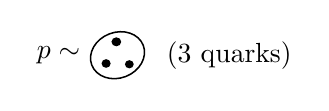
\begin{tikzpicture}[line width=.55pt]
\node at (-.75,0) {\(p\sim\)};
\draw[rotate=21] (0,0) ellipse (.35 and .29);
\fill (-.015,.17) ellipse (.062 and .057);
\fill (-.145,-.105) ellipse (.058 and .055);
\fill (.15,-.115) ellipse (.056 and .052);
\node[anchor=west] at (.50,0) {(3 quarks)};
\end{tikzpicture}}\endgroup\par
After \(p\sim\), an oval with three dots and the label “3 quarks”.}
\end{GelfandAdjacentEvidence}
\begin{GelfandAdjacentEvidence}{GELFAND-P000669}{6}

They are free inside, and it is impossible to take them out.

[crossed out: They.] \underline{Quarks are visible} --- probing
[inserted above: the proton] \(\gamma\)-quanta (as in a cellophane bag).
\Unclear{GELFAND-P000669}{they-cancel}{“They” is crossed out before “Quarks”.}
\end{GelfandAdjacentEvidence}
\begin{GelfandAdjacentEvidence}{GELFAND-P000669}{7}

\SourceFigure{GELFAND-P000669}{proton-callout}{%
\par\smallskip
\begingroup\color{black}\GelfandFitDiagram{
\begin{tikzpicture}[line width=.55pt]
\node at (0,.26) {the proton};
\draw (-.87,.36) .. controls (-.94,.13) and (-.76,.02) .. (-.47,.03)
  .. controls (-.18,.05) and (.01,-.07) .. (.01,-.23)
  .. controls (.04,-.02) and (.25,.03) .. (.58,.04)
  .. controls (.96,.05) and (.96,.50) .. (.59,.52)
  .. controls (.18,.59) and (-.45,.51) .. (-.72,.43);
\end{tikzpicture}}\endgroup\par
“The proton” is inserted before the quanta.}
\end{GelfandAdjacentEvidence}
\begin{GelfandAdjacentEvidence}{GELFAND-P000669}{8}


\underline{In the theory the forces must increase with distance!}

[crossed out] By the uncertainty princ. they cannot merge.
\Incomplete{GELFAND-P000669}{principle-cancel}{The short entry before “By the principle” is crossed out.}
\end{GelfandAdjacentEvidence}
\begin{GelfandAdjacentEvidence}{GELFAND-P000669}{9}


\underline{Relativ. inv.} hinders specifying a law of forces (the interaction potential is relativ. noninvariant).

\underline{Locality} is confirmed by probing --- quarks are nearly pointlike.

one must construct Lagrangians.

Gauge theory gives such a law of forces.

\underline{Quark} --- \underline{matrix}.
\SourceFigure{GELFAND-P000669}{quark-matrix}{%
\par\smallskip
\begingroup\color{black}\GelfandFitDiagram{\begin{tikzpicture}[line width=.5pt, every node/.style={font=\footnotesize,inner sep=1pt}]
\node (quarks) at (0,0) {\(\begin{pmatrix}
p_1&n_1&\lambda_1\\p_2&n_2&\lambda_2\\p_3&n_3&\lambda_3
\end{pmatrix}\)};
\node at (-1.42,.20) {\(G\)};
\draw[->] (-1.20,.52) -- (-1.20,-.09);
\draw (-1.64,-.77)--(-1.47,-.43) (-1.58,-.77)--(-1.41,-.43);
\node[align=center] at (-1.39,-1.16) {\(SU(3)\)\\(colour)};
\draw[->] (-.61,-.77)--(.53,-.77);
\draw[->] (.14,-1.46)--(-.05,-.92);
\node at (.46,-1.65) {group unknown.};
\node[anchor=west,align=left] at (1.11,.02) {gr. of \underline{colour}\\and gr. of \underline{flavour}.};
\end{tikzpicture}}\endgroup\par
At left \(G\) and a downward arrow. Below the matrix a rightward arrow with an annotation. The labels at right name colour and flavour.}
\end{GelfandAdjacentEvidence}
\begin{GelfandAdjacentEvidence}{GELFAND-P000669}{10}


There are 9 quarks.

Forces that prevent breaking apart are connected with colour.

\underline{To the colour gr.} corresponds [crossed out] a much stronger symm. --- \underline{gauge}.
\Incomplete{GELFAND-P000669}{color-cancel}{The isolated sign after “corresponds” is heavily crossed out.}
\end{GelfandAdjacentEvidence}


Mesons are constructed from a \underline{quark and an antiquark}.


\Needspace{7\baselineskip}
\begin{GelfandAdjacentEvidence}{GELFAND-P000670}{1}
\SourcePage{GELFAND-P000670}{unlabelled}
\underline{18/X-76.}\quad\underline{Gelfand Sem..}

[crossed out] \underline{Write down the basic notions and equations one needs to know.} \underline{And the problems.}
\Incomplete{GELFAND-P000670}{top-cancel}{The long entry before “Write down” is heavily crossed out.}
\end{GelfandAdjacentEvidence}
\begin{GelfandAdjacentEvidence}{GELFAND-P000670}{2}


\underline{\underline{Problem}}: express \(\mathrm{II}_1\) factors using matrices of continuous order.
\Unclear{GELFAND-P000670}{factor-type}{The subscript is heavily retraced. Its outline reads 1.}
\end{GelfandAdjacentEvidence}
\begin{GelfandAdjacentEvidence}{GELFAND-P000670}{3}


(undone)
\Unclear{GELFAND-P000670}{factor-parenthesis}{The note tentatively reads “не сделанная” (undone).}
\end{GelfandAdjacentEvidence}
\begin{GelfandAdjacentEvidence}{GELFAND-P000670}{4}


\underline{\underline{I. Bernstein.}} (\underline{continued}).

\underline{Superspace} --- informally, there are 2 sets of variables:
\[
\left\Vert\begin{array}{l}
x_1,\ldots,x_p,\\
\xi_1,\ldots,\xi_q
\end{array}\right.
\]
\underline{Formally}
\[
C^\infty(\mathbb R^p)\otimes\Lambda(\xi_1,\quad,\xi_q)
\]
An element:
\[
\sum f_{\alpha_1.\quad\alpha_q}(x)\xi_1^{\alpha_1}\cdots\xi_q^{\alpha_k},
\qquad \alpha_i=0,1.
\]
\Unclear{GELFAND-P000670}{last-exponent}{The last \(\xi_q\) has exponent \(\alpha_k\). The coefficient ends in subscript \(\alpha_q\).}
\end{GelfandAdjacentEvidence}
\begin{GelfandAdjacentEvidence}{GELFAND-P000670}{5}


All \(f\) commute with \(\xi\), and
\(\xi_i\xi_j=-\xi_j\xi_i,\ \xi_i^2=0\).

\(\mathbb Z_2\) --- \underline{Grading}.\qquad
\underline{Degree} --- sum of \(\alpha_i\bmod 2.\ \Vert\)

\underline{\underline{Another def.}}\qquad
[crossed out] \underline{Ringed space}.
\Incomplete{GELFAND-P000670}{ringed-cancel}{The narrow sign before “Ringed” is blacked out.}
\end{GelfandAdjacentEvidence}
\begin{GelfandAdjacentEvidence}{GELFAND-P000670}{6}


\(\mathbb R^p\) with the sheaf \(\mathcal A_{p,q}\).
\[
U\subset\mathbb R^p\quad\longmapsto\quad
\text{ring }C^\infty(U)\otimes\Lambda(\xi_1,\quad,\xi_q)
\]
\(U\subset V\quad\Rightarrow\quad\) there is a natural restriction map.

\underline{\underline{Superdomain.}} This is a topological space \(U\subset\mathbb R^p\) with the same sheaf
\[
\mathcal U=(U,\mathcal A_{p,q}).
\]
\Unclear{GELFAND-P000670}{sheaf-letter}{The symbol is repeated in the ordered pair and reads as a script \(\mathcal A\).}
\end{GelfandAdjacentEvidence}
\begin{GelfandAdjacentEvidence}{GELFAND-P000670}{7}


[Crossed out above the heading]
\Incomplete{GELFAND-P000670}{example-cancel}{The short word above “Example” is heavily crossed out.}
\end{GelfandAdjacentEvidence}
\begin{GelfandAdjacentEvidence}{GELFAND-P000670}{8}


\underline{Example.} \(u,\xi_1,\xi_2,\qquad 0<u<1\).
\SourceFigure{GELFAND-P000670}{interval}{%
\par\smallskip
\begingroup\color{black}\GelfandFitDiagram{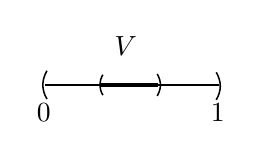
\begin{tikzpicture}[line width=.55pt]
\draw (0,0)--(2.2,0);
\draw (.02,.18) to[bend right=30] (.02,-.18);
\draw (2.17,.16) to[bend left=30] (2.17,-.19);
\draw[line width=1.2pt] (.71,0)--(1.43,0);
\draw (.73,.13) to[bend right=30] (.73,-.13);
\draw (1.42,.14) to[bend left=30] (1.42,-.14);
\node at (1.02,.49) {\(V\)};
\node at (-.02,-.35) {\(0\)};
\node at (2.19,-.35) {\(1\)};
\end{tikzpicture}}\endgroup\par
The inner interval \(V\) is marked by a heavier line between parentheses.}
\end{GelfandAdjacentEvidence}
\begin{GelfandAdjacentEvidence}{GELFAND-P000670}{9}

functions on \(V=C^\infty(V)\otimes\Lambda(\xi_1,\xi_2)\).
\[
\begin{aligned}
f_{00}(u)+[\text{crossed out}]\,
f_{10}(u)\xi_1+f_{01}\xi_2+f_{11}(u)\xi_1\xi_2.
\end{aligned}
\]
\Incomplete{GELFAND-P000670}{function-cancel}{A group of signs after \(f_{00}(u)+\) is crossed out.}
\end{GelfandAdjacentEvidence}
\begin{GelfandAdjacentEvidence}{GELFAND-P000670}{10}


\(C^\infty(\widetilde U)\) --- notation for the space of fns. on the superdomain \(\widetilde U\).
\[
\begin{gathered}
\Vert\\
C^\infty(U)\otimes\Lambda(\xi_1,\ldots,\xi_q)
\end{gathered}
\]

\underline{Map of superdomains} \(\varphi:\widetilde U\longrightarrow\widetilde V\)

this is a collection of objects: \underline{a map} \(\varphi':U\to V\)

and \underline{a map}
\[
C^\infty(\widetilde V)\longrightarrow C^\infty(\widetilde U)
\]
a ring hom. covering \(\varphi'\) (with unit) and preserving \underline{parity}!!

[crossed out: and if \(V\supset V_0\)?]
\Unclear{GELFAND-P000670}{map-cancel}{The sign between \(V\) and \(V_0\) in the crossed-out line resembles \(\supset\).}
\end{GelfandAdjacentEvidence}
\begin{GelfandAdjacentEvidence}{GELFAND-P000670}{11}


\underline{\underline{Example.}}
\SourceFigure{GELFAND-P000670}{point}{%
\par\smallskip
\begingroup\color{black}\GelfandFitDiagram{\begin{tikzpicture}
\node at (0,0) {\(U\)};
\draw[line width=.65pt] (.95,0) circle (.045);
\node at (1.51,.33) {\(1\)};
\node at (2.07,0) {\(\xi_1,\xi_2\)};
\end{tikzpicture}}\endgroup\par
Beside the point are the labels \(U\), \(1\) and \(\xi_1,\xi_2\).}
\end{GelfandAdjacentEvidence}
\begin{GelfandAdjacentEvidence}{GELFAND-P000670}{12}

\underline{\(p=0,\ q=2\).}\qquad Superdomain of dimension \((0,2)\).

Geometrically, a point. a map of the superdomain to itself is an endomorphism.

Rings \(\Lambda(\xi_1,\xi_2)\).
\SourceFigure{GELFAND-P000670}{parity-cancel}{%
\par\smallskip
\begingroup\color{black}\GelfandFitDiagram{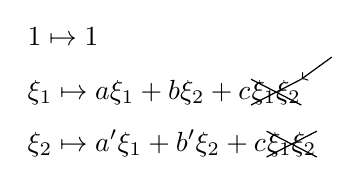
\begin{tikzpicture}[line width=.45pt, every node/.style={inner sep=0}]
\node[anchor=base west] at (0,.73) {\(1\mapsto1\)};
\node[anchor=base west] (first) at (0,.05) {\(\xi_1\mapsto a\xi_1+b\xi_2+c\)};
\node[anchor=base west] (second) at (0,-.61) {\(\xi_2\mapsto a'\xi_1+b'\xi_2+c\)};
\node[anchor=base west] (producta) at (first.base east) {\(\xi_1\xi_2\)};
\node[anchor=base west] (productb) at (second.base east) {\(\xi_1\xi_2\)};
\foreach \term in {producta,productb}{
  \draw (\term.north west) -- (\term.south east)
        (\term.south west) -- (\term.north east);
}
\draw[->] ([xshift=11pt,yshift=8pt]producta.north east) -- (producta.north east);
\end{tikzpicture}}\endgroup\par
The arrowed note reads “disallowed, since it preserves parity”. The letter \(c\) follows the final plus, before the crossed-out product. A prime is unclear.}
\end{GelfandAdjacentEvidence}


\underline{\underline{\(a,b,a',b'\)}} --- arbitrary.


\Needspace{7\baselineskip}
\begin{GelfandAdjacentEvidence}{GELFAND-P000671}{1}
\SourcePage{GELFAND-P000671}{unlabelled}
\underline{The algebra} \(\Lambda(\xi_1,\xi_2)\) \underline{is commutative in the super sense}.
\[
xy=(-1)^{p(x)p(y)}yx.
\]

\underline{Example 2.}
\[
\begin{array}{l}
u,\xi_1,\xi_2\\
v,\eta_1,\eta_2
\end{array}
\qquad
\left\Vert\begin{aligned}
v&=u+\xi_1\xi_2\\
\eta_1&=\xi_1\\
\eta_2&=\xi_2.
\end{aligned}\right.
\]
\underline{Problem:} what is the image of \(\sin v\)?

An element of the left ring has the form
\[
f_{00}(u)+f_{10}(u)\xi_1+f_{01}(u)\xi_2+f_{11}(u)\xi_1\xi_2
\]
An elem. of the 2nd ring
\[
g_{00}(v)+g_{10}(v)\xi_1+g_{01}(v)\xi_2+g_{11}(v)\xi_1\xi_2
\]
\Unclear{GELFAND-P000671}{second-ring}{The 2nd ring is written with \(\xi_1,\xi_2\), as in the 1st.}
\end{GelfandAdjacentEvidence}
\begin{GelfandAdjacentEvidence}{GELFAND-P000671}{2}


\underline{map}
\[
\begin{gathered}
\widetilde U\longrightarrow\widetilde V\\
C^\infty(\widetilde V)\longrightarrow C^\infty(\widetilde U)\\
g_{00}(v)\mapsto g_{00}(u+\xi_1\xi_2)=g_{00}(u)+\xi_1\xi_2g'_{00}(u).
\end{gathered}
\]

\(x=(u_1,\ldots,u_p,\xi_1,\ldots,\xi_q)\) --- a coordinate system.
\[
\frac{\partial}{\partial u_i}f\xi_1^{\alpha_1}\ldots\xi_q^{\alpha_q}
=\frac{\partial f}{\partial u_i}\xi_1^{\alpha_1}\ldots\xi_q^{\alpha_q}
\]

\underline{Stokes’ theorem --- ?}

The integral of a superfunction over a superdomain.

\underline{Analogue in ordinary analysis}
\SourceFigure{GELFAND-P000671}{oval-diagram}{%
\par\smallskip
\begingroup\color{black}\GelfandFitDiagram{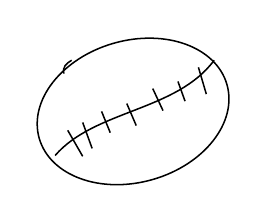
\begin{tikzpicture}[line width=.55pt]
\draw[rotate=16] (0,0) ellipse (1.24 and .90);
\draw (-.99,-.56) .. controls (-.49,.02) and (.55,.00) .. (1.03,.65);
\draw (-.83,-.24)--(-.64,-.57) (-.64,-.14)--(-.52,-.47)
      (-.40,.00)--(-.29,-.27) (-.08,.10)--(.04,-.18)
      (.25,.29)--(.38,.01) (.57,.38)--(.66,.13)
      (.83,.56)--(.93,.22);
\draw (-.88,.48) .. controls (-.90,.56) and (-.85,.61) .. (-.78,.65);
\end{tikzpicture}}\endgroup\par
A rising curve and seven visible cross-strokes lie inside the oval. A short mark meets the outline at the upper left.}
\end{GelfandAdjacentEvidence}
\begin{GelfandAdjacentEvidence}{GELFAND-P000671}{3}


jets in a nbhd. of a submanifold.
\Unclear{GELFAND-P000671}{middle-phrase}{The first words read “струи в окр.” (jets in a nbhd.). The start of “submanifold” is retraced.}
\end{GelfandAdjacentEvidence}
\begin{GelfandAdjacentEvidence}{GELFAND-P000671}{4}


The integral for fns. on a manifold with boundary is noninv. under changes of variables.

Difference: here one cannot integrate forms. One can integrate densities (under change of coords. mult. by the \underline{Berezinian}).

\underline{\underline{What does one integrate over the boundary?}}

\(\underline{\underline{U,\partial U}}.\)\quad
\(f=0\), where \(f\in C^\infty(U)\) --- \underline{a superfunction}.

\underline{Closed superdomain.}\quad \(\underline{\underline{u,\xi_1,\xi_2}}\)
\SourceFigure{GELFAND-P000671}{boundary-arrow}{%
\par\smallskip
\begingroup\color{black}\GelfandFitDiagram{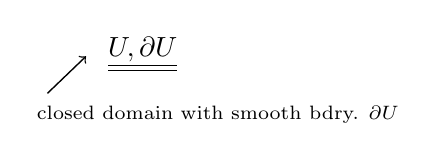
\begin{tikzpicture}[line width=.5pt]
\node at (.94,.44) {\(\underline{\underline{U,\partial U}}\)};
\node[anchor=west] at (-.53,-.32) {\scriptsize closed domain with smooth bdry. \(\partial U\)};
\draw[->] (-.27,-.05)--(.22,.42);
\end{tikzpicture}}\endgroup\par
The arrow points from the note towards \(U,\partial U\).}
\end{GelfandAdjacentEvidence}
\begin{GelfandAdjacentEvidence}{GELFAND-P000671}{5}


On \(\partial U\) there is the struct. of a [inserted above: sub] supermanifold.
\SourceFigure{GELFAND-P000671}{lower-supermanifold}{%
\par\smallskip
\begingroup\color{black}\GelfandFitDiagram{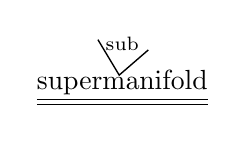
\begin{tikzpicture}[line width=.5pt]
\node (word) at (0,0) {\underline{\underline{supermanifold}}};
\node at (0,.57) {\scriptsize sub};
\draw (-.31,.62) -- (-.04,.17) -- (.33,.49);
\end{tikzpicture}}\endgroup\par
The “sub” insertion points after “super”. The ending of the abbreviation is tentative.}
\end{GelfandAdjacentEvidence}
\begin{GelfandAdjacentEvidence}{GELFAND-P000671}{6}


(by an even \underline{eq.} [crossed out: this?] \underline{is cut out})
\Unclear{GELFAND-P000671}{lower-cancellation}{The crossed-out word tentatively reads “это” (this).}
\end{GelfandAdjacentEvidence}
\begin{GelfandAdjacentEvidence}{GELFAND-P000671}{7}


\(\underline{\underline{[0,\infty)}}\qquad \underline{\underline{u,\xi_1,\xi_2.}}\)

Different superdomains
\[
\begin{aligned}
1.\quad &u=0\\
2.\quad &u+c\xi_1\xi_2=0
\end{aligned}
\]
\SourceFigure{GELFAND-P000671}{bottom-diagram}{%
\par\smallskip
\begingroup\color{black}\GelfandFitDiagram{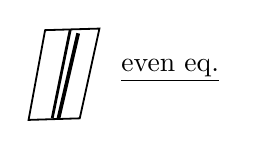
\begin{tikzpicture}[line width=.65pt]
\draw (-.40,0)--(-.19,1.14)--(.50,1.16)--(.25,.02)--cycle;
\draw[line width=1.0pt] (-.10,.02)--(.13,1.15);
\draw[line width=1.35pt] (-.02,.02)--(.23,1.10);
\node[anchor=west] at (.65,.62) {\underline{even eq.}};
\end{tikzpicture}}\endgroup\par
A narrow slanted quadrilateral with heavy lengthwise strokes. The words at right label the figure.}
\end{GelfandAdjacentEvidence}



\Needspace{7\baselineskip}
\begin{GelfandAdjacentEvidence}{GELFAND-P000672}{1}
\SourcePage{GELFAND-P000672}{unlabelled}
\underline{\underline{Submanifold:}} \underline{in the ring choose an ideal of fns..}

Boundary --- \underline{even}.

\(C^\infty(\widetilde U)\)\qquad Boundary --- \underline{eq.}
\(\underline{\underline{f(\widetilde U)=0}}\)
\[
\int \text{of a compactly supported fn.}=\int f_{11\ldots1}\,du_1\ldots du_p
\]

\underline{Different for closed domains.}

Let the half-space be \(\underline{\underline{u_1\ge0}}\)

Then the integr. is given by the same formula.

It is preserved if it maps into itself as a supermanifold.

\(u_1^2+u_2^2\le1\)
\SourceFigure{GELFAND-P000672}{disk}{%
\par\smallskip
\begingroup\color{black}\GelfandFitDiagram{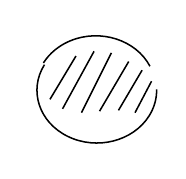
\begin{tikzpicture}[line width=.55pt]
\draw (.68,.30) arc (25:151:.76 and .67);
\draw (-.66,.32) arc (151:361:.76 and .67);
\draw (-.59,-.12)--(-.26,.43) (-.43,-.24)--(-.03,.49)
      (-.19,-.29)--(.19,.47) (.04,-.27)--(.41,.36)
      (.28,-.26)--(.58,.25) (.49,-.29)--(.70,.11);
\end{tikzpicture}}\endgroup\par
Slanted strokes fill the disc.}
\end{GelfandAdjacentEvidence}
\begin{GelfandAdjacentEvidence}{GELFAND-P000672}{2}

\[
\begin{gathered}
u_1^2+u_2^2-1=0\quad(1)\quad\text{--- 2 boundaries}\\
u_1^2+u_2^2-1-\xi_1\xi_2=0\quad(2)
\end{gathered}
\]
Integral over the domain with boundary (2).
\[
\int[f_{00}(u)+f_{01}(\ )\xi_1+\ldots]
\]
\Unclear{GELFAND-P000672}{integrand-subscript}{After \(f_{01}\) the parentheses are empty, followed by \(\xi_1\).}
\end{GelfandAdjacentEvidence}
\begin{GelfandAdjacentEvidence}{GELFAND-P000672}{3}


\underline{Roughly}
\[
\int\xi_1\xi_2\,d\xi_1\,d\xi_2=1
\]

--- For the ordinary boundary ---
\[
\int_{u_1^2+u_2^2<1}f_{11}(u)\,du_1du_2
\]

\underline{Check of invariance} --- the boundary eq. must stay the same.

If the boundary is \(\underline{u_1^2+u_2^2-1-\xi_1\xi_2=0}\)

change variables so the boundary goes to the normal one
\[
\underline{\left(u_1-\tfrac12\xi_1\xi_2\right)^2+u_2^2-1=0.}
\]
\Unclear{GELFAND-P000672}{shifted-circle}{Inside the parentheses the term after \(u_1\) is \(-\frac12\xi_1\xi_2\).}
\end{GelfandAdjacentEvidence}
\begin{GelfandAdjacentEvidence}{GELFAND-P000672}{4}


[crossed out: \(u=0\)?]
\Unclear{GELFAND-P000672}{upper-cancellation}{The crossed-out formula above the line tentatively reads \(u=0\).}
\end{GelfandAdjacentEvidence}
\begin{GelfandAdjacentEvidence}{GELFAND-P000672}{5}


\SourceFigure{GELFAND-P000672}{half-line}{%
\par\smallskip
\begingroup\color{black}\GelfandFitDiagram{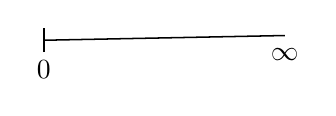
\begin{tikzpicture}[line width=.55pt]
\draw (0,0)--(3.06,.06);
\draw (0,-.15)--(0,.15);
\node[below] at (0,-.13) {\(0\)};
\node[below] at (3.06,.02) {\(\infty\)};
\end{tikzpicture}}\endgroup\par
A tick and \(0\) mark the left end. The right end is marked \(\infty\).}
\end{GelfandAdjacentEvidence}
\begin{GelfandAdjacentEvidence}{GELFAND-P000672}{6}

\[
\int_0^\infty f_{11}(u)\,du\qquad u,\xi_1,\xi_2
\]
bdry. \(u=0\).

\(\underline{v=u+u\xi_1\xi_2.}\)

The boundary will be \(\underline{\underline{v=0}}\)
\[
\begin{aligned}
\int_0^\infty g_{11}(v)\,dv
&=\int_0^\infty g_{11}(u+u\xi_1\xi_2)\,dv\\
&=\int_0^\infty g_{11}(u)\,dv
  +\int_0^\infty g'_{11}(u)u\xi_1\xi_2\,dv
\end{aligned}
\]
\Unclear{GELFAND-P000672}{integral-differentials}{The differential in the third integral resembles \(dv\).}
\end{GelfandAdjacentEvidence}
\begin{GelfandAdjacentEvidence}{GELFAND-P000672}{7}


\SourceFigure{GELFAND-P000672}{integral-sketch}{%
\par\smallskip
\begingroup\color{black}\GelfandFitDiagram{
\begin{tikzpicture}[line width=.55pt]
\draw (-.35,.91) .. controls (-.04,.22) and (.55,-.05) .. (1.15,-.45);
\draw (-.36,.82) .. controls (-.57,.52) and (-1.10,-.03) .. (-1.07,-.18)
  .. controls (-.95,-.22) and (-.56,.43) .. (-.29,.62);
\draw (-.26,.62) .. controls (-.59,.16) and (-.98,-.25) .. (-.88,-.32)
  .. controls (-.73,-.32) and (-.52,.02) .. (-.34,.18);
\draw (-.49,-.11) .. controls (.22,.77) and (.48,.73) .. (.27,.21)
  .. controls (.06,-.16) and (-.48,-.52) .. (-.42,-.58)
  .. controls (-.22,-.66) and (.49,.12) .. (.71,.18)
  .. controls (1.04,.26) and (.68,-.40) .. (.21,-.79);
\end{tikzpicture}}\endgroup\par
An open descending curve with diagonal and looping strokes. Some of their junctions are indistinct.}
\end{GelfandAdjacentEvidence}
\begin{GelfandAdjacentEvidence}{GELFAND-P000672}{8}

\[
\frac{Dv}{Du}
\]
\underline{Integral over a domain with boundary ---}

\underline{--- Bernstein and Leites}

[crossed out]
\Incomplete{GELFAND-P000672}{lower-cancellation}{The word before “There is work” is heavily crossed out.}
\end{GelfandAdjacentEvidence}
\begin{GelfandAdjacentEvidence}{GELFAND-P000672}{9}


There is work by \underline{Berezin} and Marinov (?)
\Unclear{GELFAND-P000672}{marinov}{The surname tentatively reads “Маринова” (Marinov). The question mark is in the manuscript.}
\end{GelfandAdjacentEvidence}


\underline{class. mech. in Fermi and Bose variables}

\underline{\underline{Problem}}: Stokes’ thm. for the circle \(u_1^2+u_2^2+c\xi_1\xi_2-1=0\).


\Needspace{7\baselineskip}
\begin{GelfandAdjacentEvidence}{GELFAND-P000673}{1}
\SourcePage{GELFAND-P000673}{unlabelled}
\underline{Notes on I. Bernstein’s previous super talks}

\uline{(from I. Dorfman’s notebook)}
\Unclear{GELFAND-P000673}{notebook-author}{The name in parentheses tentatively reads “И. Дорфман” (I. Dorfman).}
\end{GelfandAdjacentEvidence}
\begin{GelfandAdjacentEvidence}{GELFAND-P000673}{2}


\underline{Def.} \underline{Superring}
\[
A=\underset{\substack{\vert\\\text{even}}}{A_0}\oplus
  \underset{\substack{\vert\\\text{odd}}}{A_1}
\qquad
\begin{aligned}
 A_0A_0&\subset A_0\\
 A_0A_1&\subset A_1\\
 A_1A_0&\subset A_1\\
 A_1A_1&\subset A_0.
\end{aligned}
\]

It is called \underline{commutative}, if
\(\underline{ab=ba(-1)^{\deg a\cdot\deg b}}\)

\underline{Linear algebra.}
\Incomplete{GELFAND-P000673}{cancelled-glyph}{Crossed-out mark before the bracket.}
\end{GelfandAdjacentEvidence}
\begin{GelfandAdjacentEvidence}{GELFAND-P000673}{3}

[Over a commut. superring consider
\Incomplete{GELFAND-P000673}{cancelled-word-one}{Crossed-out word after “consider”.}
\end{GelfandAdjacentEvidence}
\begin{GelfandAdjacentEvidence}{GELFAND-P000673}{4}

any \(A\)-module \(A^n\) and its
\Incomplete{GELFAND-P000673}{cancelled-word-two}{Crossed-out word after “its”.}
\end{GelfandAdjacentEvidence}
\begin{GelfandAdjacentEvidence}{GELFAND-P000673}{5}

endomorphism given by a block matrix]
\[
[A=]\begin{pmatrix}A_{11}&A_{12}\\ A_{21}&A_{22}\end{pmatrix}
\qquad
\det A\underset{\mathrm{def}}{=}
\det A_{11}^{-1}\det(A_{22}-A_{21}A_{11}^{-1}A_{12})
\]
\Unclear{GELFAND-P000673}{determinant-reciprocal}{The faint superscript on the first \(A_{11}\) reads \(-1\).}
\end{GelfandAdjacentEvidence}
\begin{GelfandAdjacentEvidence}{GELFAND-P000673}{6}

\[
\begin{gathered}
\operatorname{str}A=\operatorname{tr}A_{11}-\operatorname{tr}A_{22}.\\
(\text{supertrace})
\end{gathered}
\]

\underline{Properties:}
\[
\begin{gathered}
\det XY=\det X\cdot\det Y.\\
\det X=\exp\operatorname{str}\ln X
\end{gathered}
\]
\Unclear{GELFAND-P000673}{logarithm-tail}{After \(X\) there is a dark mark below the line. It may be a comma or a crossed-out sign.}
\end{GelfandAdjacentEvidence}
\begin{GelfandAdjacentEvidence}{GELFAND-P000673}{7}

\[
\begin{gathered}
\operatorname{str}(XY)=\operatorname{str}(YX)\\
\begin{pmatrix}A&B\\ C&D\end{pmatrix}^{*}
=\begin{pmatrix}A^{*}&C^{*}\\ -B^{*}&D^{*}\end{pmatrix}
\end{gathered}
\]

\underline{Superanalysis.}

Consider
\[
\sum f_{i_1\quad i_k}(x_1,\mathord{-},x_p)\,
\xi_1^{i_1}\ldots\xi_k^{i_k}
\]
\Unclear{GELFAND-P000673}{expansion-mark}{A faint short stroke appears between the commas after \(x_1\).}
\end{GelfandAdjacentEvidence}
\begin{GelfandAdjacentEvidence}{GELFAND-P000673}{8}


Rules of differentiation
\[
\begin{gathered}
\frac{\partial}{\partial\xi_1}(\xi_1\xi_2)=\xi_2,\qquad
\frac{\partial}{\partial\xi_2}(\xi_1\xi_2)=-\xi_1,\\
\frac{\partial}{\partial\xi_1}\xi_2=0,\qquad
\frac{\partial}{\partial\xi_1}\xi_1=1,\qquad
\frac{\partial}{\partial\xi_1}1=0.
\end{gathered}
\]

\noindent\rule{12mm}{.45pt}\enspace\(\cdot\)\enspace\rule{14mm}{.45pt}

Consider block matrices \(\begin{pmatrix}A&B\\ C&D\end{pmatrix}\)
\[
\begin{aligned}
A&=A_{\bar{0}}\oplus A_{\bar{1}}\\
\mathbb Z/2\mathbb Z&\text{ --- grad.}\\
\bar{0},\bar{1}&\text{ --- elem.}\\
p(a)&\text{ --- parity}
\end{aligned}
\qquad
\begin{aligned}
\text{elem. }A,D&\in A_{\bar{0}}\\
\text{elem. }B,C&\in A_{\bar{1}}
\end{aligned}
\]
\[
\begin{gathered}
\operatorname{Ber}J=(\det D)^{-1}\cdot\det(A-BD^{-1}C)\in A_{\bar{0}}\\
(\text{Berezinian})
\end{gathered}
\]

\underline{Assert}
\[
\begin{gathered}
\operatorname{Ber}J_1J_2=\operatorname{Ber}J_1\cdot\operatorname{Ber}J_2.\\
\operatorname{str}J=\operatorname{tr}A-\operatorname{tr}D
\end{gathered}
\]
\underline{Assert.}
\[
\operatorname{str}(J_1J_2)=\operatorname{str}(J_2J_1).
\]

\noindent\rule{11mm}{.45pt}\enspace\(\cdot\)\enspace\rule{15mm}{.45pt}

In \(\mathbb R^p\) consider \(C^\infty(\mathbb R^p)\otimes\Lambda(\xi_1,\mathord{\text{---}},\xi_q)\)
\SourceFigure{GELFAND-P000673}{exterior-arrow}{%
\par\smallskip
\begingroup\color{black}\GelfandFitDiagram{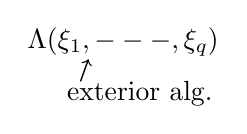
\begin{tikzpicture}[line width=.5pt]
\node[anchor=west,inner sep=0pt] at (0,.65)
  {\(\Lambda(\xi_1,\mathord{\text{---}},\xi_q)\)};
\node[anchor=west,inner sep=0pt] at (.50,0) {exterior alg.};
\draw[->] (.68,.15)--(.78,.43);
\end{tikzpicture}}\endgroup\par
The arrow from the note points up towards the comma after \(\xi_1\).}
\end{GelfandAdjacentEvidence}


\(p(\xi_i)=1,\qquad \xi_i\xi_j=-\xi_j\xi_i.\)


\Needspace{7\baselineskip}
\begin{GelfandAdjacentEvidence}{GELFAND-P000674}{1}
\SourcePage{GELFAND-P000674}{unlabelled}
\[
\Lambda(\xi_1,\ldots,\xi_q)\ni\xi_1^{\alpha_1}\cdots\xi_q^{\alpha_q},
\qquad \alpha_i=0,1.
\]
\[
f=\sum f_{\alpha_1\alpha_2\ldots\alpha_q}\,
     \xi_1^{\alpha_1}\cdots\xi_q^{\alpha_q}.
\]

\underline{Def.}
\[
\mathbb R^{p,q}=
\left(\mathbb R^p,C^\infty(\mathbb R^p)\otimes\Lambda(\xi_1,\ldots,\xi_q)\right)
\]
--- superspace of dim. \((p,q)\).

\underline{Def.}
\[
U=\left(u,\underbrace{C^\infty(u)\otimes\Lambda(\xi_1,\ldots,\xi_q)}
                        _{(\mathrm{def})\, C^\infty(U)}\right)
\]
\uwave{superdomain.}

(ringed sp.!)

--- ring of fns. on the dom.
\Unclear{GELFAND-P000674}{upper-ring-abbreviation}{The abbreviation after “on” tentatively reads “обл.” (dom.).}
\end{GelfandAdjacentEvidence}
\begin{GelfandAdjacentEvidence}{GELFAND-P000674}{2}

\SourceFigure{GELFAND-P000674}{ring-definition-callout}{
\par\smallskip
\begingroup\color{black}\GelfandFitDiagram{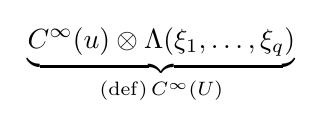
\begin{tikzpicture}
\node[inner sep=0pt] {\(\underbrace{C^\infty(u)\otimes\Lambda(\xi_1,\ldots,\xi_q)}
                              _{(\mathrm{def})\,C^\infty(U)}\)};
\end{tikzpicture}}\endgroup\par
The brace under the tensor product points to \((\mathrm{def})\, C^\infty(U)\).}
\end{GelfandAdjacentEvidence}
\begin{GelfandAdjacentEvidence}{GELFAND-P000674}{3}


map \(\widetilde{\psi}:U\to V\)
\Unclear{GELFAND-P000674}{upper-morphism-letter}{The isolated mark before the dash is undeciphered.}
\end{GelfandAdjacentEvidence}
\begin{GelfandAdjacentEvidence}{GELFAND-P000674}{4}

--- morphism of ringed sp. ---
this is a map
\Incomplete{GELFAND-P000674}{upper-map-cancellation}{Crossed-out writing before \(\psi\).}
\end{GelfandAdjacentEvidence}
\begin{GelfandAdjacentEvidence}{GELFAND-P000674}{5}

\[
\psi:C^\infty(V)\to C^\infty(U).
\]
\Unclear{GELFAND-P000674}{pullback-rings}{The arguments in the function rings are rendered as \(V\) and \(U\). The manuscript barely distinguishes their case.}
\end{GelfandAdjacentEvidence}
\begin{GelfandAdjacentEvidence}{GELFAND-P000674}{6}


\underline{Coord. notation.} Let a tuple be chosen in the sp. \(U\)
\[
(u_1,\ldots,u_p,\xi_1,\ldots,\xi_q)
\]
\hspace*{2em}--- \textquotedbl{} --- \(V\) --- \textquotedbl{} ---
\((v_1,\ldots,v_m,\eta_1,\ldots,\eta_n)\).

It turns out that to specify the map \(\psi:U\to V\)
\Incomplete{GELFAND-P000674}{middle-map-cancellation}{Crossed-out word after \(U\to V\).}
\end{GelfandAdjacentEvidence}
\begin{GelfandAdjacentEvidence}{GELFAND-P000674}{7}

it suffices to specify
\[
v_1^*,\ldots,v_m^*,\eta_1^*,\ldots,\eta_n^*.
\]

\underline{Example.}
\[
\begin{aligned}
v&=u+\xi_1\xi_2\\
\eta_1&=u\xi_1\\
\eta_2&=\xi_2.
\end{aligned}
\]
\underline{Problem.} What is the form of \(\sin v\)?

\underline{Assert.}
\[
\frac{\partial}{\partial u_i}(f\xi^\alpha)
=\frac{\partial f}{\partial u_i}\cdot\xi^\alpha,
\]
\[
\begin{aligned}
\frac{\partial}{\partial\xi_j}
  (f\xi_1^{\alpha_1}\cdots\xi_q^{\alpha_q})
&=\alpha_j(-1)^{\alpha_1+\ldots+\alpha_{j-1}}\,
  f\xi_1^{\alpha_1}\cdots\widehat{\xi}_j^{\alpha_j}\cdots\xi_q^{\alpha_q}.
\end{aligned}
\]
\Unclear{GELFAND-P000674}{odd-derivative-omission}{The omission mark is over \(\xi_j\), with \(\alpha_j\) still written at upper right. The final \(q\) is retraced.}
\end{GelfandAdjacentEvidence}


\noindent\rule{23mm}{.45pt}\enspace\(\cdot\)\enspace\rule{17mm}{.45pt}

Let \(U\) be a superdomain
\[
\begin{aligned}
x&=(u,\xi)\\
y&=(v,\eta)
\end{aligned}
\]
\[
J=(J_{ij}),\qquad J_{ij}=\frac{\partial y_j}{\partial x_i}.
\]
\[
\operatorname{Ber}J\underset{\mathrm{def}}{=}D(y)/D(x).
\]

\underline{Def.} \(U\), \(x=(u,\xi)\).

The expr. \(\rho=fD(x)\) is called a \uwave{volume form}.
\[
fD(x)=f\bigl(D(x)/D(y)\bigr)\cdot D(y).
\]

\underline{Definition.}
\[
\int_u fD(x)\underset{\mathrm{def}}{=}
\int_u f_{11\ldots1}(u)\,du_1\ldots du_p
\]
(integral of a volume form)

\underline{Theorem (Berezin)} This expr. is independent of the coordinate system.

Here one integrates a compactly supported fn.


\Needspace{7\baselineskip}
\begin{GelfandAdjacentEvidence}{GELFAND-P000675}{1}
\SourcePage{GELFAND-P000675}{unlabelled}
\underline{25/X-76.}\qquad \underline{Gelfand seminar.}

\underline{Gelfand.}

\underline{What is a connection?} (for first-year students and Polyakov).

--- see Nomizu, Sternberg, Bishop and Crittenden, Landau and Lifshitz.

\uwave{Popov.}

\underline{The founders’ paper} (Yang, Mills --- translation in the coll. “Elem. particles and compensating fields”).

Consider the Dirac eq.

{\small without mass}
\SourceFigure{GELFAND-P000675}{dirac-grouping}{%
\par\smallskip
\begingroup\color{black}\GelfandFitDiagram{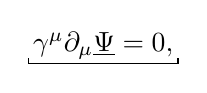
\begin{tikzpicture}[baseline=(eq.base),line width=.45pt]
\node[inner sep=1.5pt] (eq) {\(\gamma^\mu\partial_\mu\underline{\Psi}=0,\)};
\draw ([yshift=2pt]eq.south west)--(eq.south west)--
      (eq.south east)--([yshift=2pt]eq.south east);
\end{tikzpicture}}\endgroup}
\end{GelfandAdjacentEvidence}
\begin{GelfandAdjacentEvidence}{GELFAND-P000675}{2}

\(\Psi=(\Psi_\alpha)\) --- ordinary 4-comp. spinor.

Yang–Mills equations:
\[
\underline{\partial_\nu F_a^{\mu\nu}+f^b_{ac}F_b^{\mu\nu}A_\nu^c=0},
\]
\Unclear{GELFAND-P000675}{upper-ym-constant}{The retraced indices on the coefficient tentatively read \(f^b_{ac}\).}
\end{GelfandAdjacentEvidence}
\begin{GelfandAdjacentEvidence}{GELFAND-P000675}{3}

where
\[
F_{\mu\nu}^a=\partial_\mu A_\nu^a-\partial_\nu A_\mu^a
+\tfrac12 f_{bc}^a(A_\mu^b A_\nu^c-A_\nu^b A_\mu^c)
\]
on \(\mathbb R^4\) consider the Minkowski metric \(g_{\mu\nu},\quad A_\mu^\alpha,\quad a=1,\ldots,\dim G\)
\Unclear{GELFAND-P000675}{potential-index}{The superscript on \(A_\mu\) is \(\alpha\). The range immediately after it uses \(a\).}
\end{GelfandAdjacentEvidence}
\begin{GelfandAdjacentEvidence}{GELFAND-P000675}{4}


(\(G\) --- some group, usually taken to be semisimple).

lowering of indices in the eq. with the aid of
\[
K_{ab}=f_{ac}^d f_{bd}^c,
\]
where \(f_{ac}^d\) --- struct. const. of the Lie algebra of the group.

\noindent\rule{9mm}{.45pt}\enspace\(\cdot\)\enspace\rule{12mm}{.45pt}

\underline{\underline{G.}} On quarks see \underline{Zel’dovich}’s article in UFN, \uwave{“Quarks for pedestrians”}.

\noindent\rule{9mm}{.45pt}\enspace\(\cdot\)\enspace\rule{12mm}{.45pt}

The Yang–Mills eqs. describe quarks.

\(\mu,\nu=1,\ldots,4\);
\Incomplete{GELFAND-P000675}{middle-cancellation}{Crossed-out writing before \(F_a^{\mu\nu}\).}
\end{GelfandAdjacentEvidence}
\begin{GelfandAdjacentEvidence}{GELFAND-P000675}{5}

\(F_a^{\mu\nu}\) --- tensor with values in the Lie algebra.

\(A\) --- analogue of the vect. potential
\[
\partial_\nu=\partial/\partial x^\nu.
\]
\(F\) --- analogue of the field-strength tensor.

\underline{Example.}

For \(G=U(1)\) one obtains the eqs. of electrodynamics.

\underline{Equations:}
\[
\left.
\begin{aligned}
\partial_\mu F^{\mu\nu}&=0\\
F^{\mu\nu}&\underset{\mathrm{def}}{=}\partial_\mu A_\nu-\partial_\nu A_\mu
\end{aligned}
\right\Vert
\]
We get Maxwell’s eqs.

\noindent\rule{10mm}{.45pt}\enspace\(\cdot\)\enspace\rule{12mm}{.45pt}

\underline{Gauge transformations.}

\underline{In the el. and magn. field:}
\[
\begin{pmatrix}
0&H_{12}&H_{13}&E_1\\
-H_{12}&0&H_{23}&E_2\\
-H_{13}&-H_{23}&0&E_3\\
-E_1&-E_2&-E_3&0
\end{pmatrix}
=F^{\mu\nu};
\]
\underline{2-form}
\Unclear{GELFAND-P000675}{field-diagonal}{The third diagonal entry is retraced and reads as zero.}
\end{GelfandAdjacentEvidence}
\begin{GelfandAdjacentEvidence}{GELFAND-P000675}{6}


\underline{Maxwell’s equations:}
\[
F^{\mu\nu}=\frac{\partial}{\partial x^\mu}A_\nu
           -\frac{\partial}{\partial x^\nu}A_\mu.
\]
--- \underline{tensor}
\Incomplete{GELFAND-P000675}{lower-tensor-cancellation}{Crossed-out writing after “tensor”.}
\end{GelfandAdjacentEvidence}
\begin{GelfandAdjacentEvidence}{GELFAND-P000675}{7}

\underline{of 2nd ord.}

Transformations of \(A\) that leave \(F\) unchanged are called gradient transformations.
\[
A_\mu\to A_\mu+\partial_\mu\alpha
\]
\SourceFigure{GELFAND-P000675}{lower-gradient-cancellation}{%
\par\smallskip
\begingroup\color{black}\GelfandFitDiagram{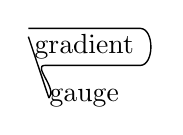
\begin{tikzpicture}[line width=.5pt]
\node[inner sep=2pt] (new) at (0,0) {gradient};
\node[inner sep=0pt] (old) at (0,-.65) {\sout{gauge}};
\draw (new.north west)--(new.north east)
  to[out=0,in=0] (new.south east)
  --([xshift=6pt]new.south west) to[out=180,in=45] (old.west);
\draw ([yshift=-3pt]new.north west)--(old.west);
\end{tikzpicture}}\endgroup\par
The outline of “gradient” points to the crossed-out abbreviation, tentatively “калибр.” (gauge).}
\end{GelfandAdjacentEvidence}



\Needspace{7\baselineskip}
\begin{GelfandAdjacentEvidence}{GELFAND-P000676}{1}
\SourcePage{GELFAND-P000676}{unlabelled}
Let \((T_a)\) be a basis in the Lie algebra \(\mathcal L(G)\).

Consider
\[
B_\mu=T_a A_\mu^a\quad\text{--- }\text{\uwave{field of matrices}.}
\]
\[
F_{\mu\nu}=T_a F_{\mu\nu}^a\quad\text{---\quad--- \textquotedbl{} ---}.
\]

\uwave{Gauge transf. on fields of matrices:}
\[
B_\mu\to B'_\mu=S^{-1}B^\mu S+S^{-1}\partial_\mu S,
\]
\Unclear{GELFAND-P000676}{gauge-index}{Between \(S^{-1}\) and \(S\), \(\mu\) is written as a superscript on \(B\).}
\end{GelfandAdjacentEvidence}
\begin{GelfandAdjacentEvidence}{GELFAND-P000676}{2}

\[
F_{\mu\nu}^{\text{\scriptsize[crossed out]}}
\to F'_{\mu\nu}=S^{-1}F_{\mu\nu}S,
\]
\Incomplete{GELFAND-P000676}{upper-f-cancellation}{Crossed-out mark above the first \(F\).}
\end{GelfandAdjacentEvidence}
\begin{GelfandAdjacentEvidence}{GELFAND-P000676}{3}

where \(S:\mathbb R^4\to G\).

Direct calculation readily shows that the eqs. are inv. under these transformations.

Unknowns --- \(A\).

Nonlinearity due to the noncommut. group.

(\(F\) --- curvature of the connection)

\uwave{Yang–Mills equations.}

Let \((P,M,G)\) be a principal bundle

(\(M\) --- manifold

\(G\) --- group
\Incomplete{GELFAND-P000676}{middle-group-cancellation}{Crossed-out writing after “group”.}
\end{GelfandAdjacentEvidence}
\begin{GelfandAdjacentEvidence}{GELFAND-P000676}{4}

--- arbitrary)

on \(M\) there is a pseudo-Riemannian metric \(g\).

In the principal bundle a connection is given by the form \(\Omega\in\mathcal L(G)\otimes\Lambda^1(P)\).

The eq. will be for this form.

Fix an arbitrary (nondegenerate) quadratic form \(K\) on the Lie algebra \(\mathcal L(G)\).

From these data a natural metric is constructed on \(P\).
\[
\begin{aligned}
h_p(Y_p,Y'_p)
&=g_{\pi(p)}(d\pi Y_p,d\pi Y'_p)\\
&\quad+K\bigl(\Omega(Y_p),\Omega(Y'_p)\bigr)
\end{aligned}
\]
in general the metric is noninvariant.

\uwave{Curvature of the connection.}
\[
\underline{\Phi=H\,d\Omega}\,,\ =d\Omega+\tfrac12[\Omega,\Omega]
\]
\Unclear{GELFAND-P000676}{lower-curvature-punctuation}{The low mark after \(d\Omega\) before the second equality is rendered as a comma.}
\end{GelfandAdjacentEvidence}
\begin{GelfandAdjacentEvidence}{GELFAND-P000676}{5}

\(H\) --- operator taking the horiz. part of a form, constructed from the connection.

\uwave{Yang–Mills equation for the free field}
\[
\boxed{H\delta_{\text{\scriptsize[crossed out]}}\varphi=0}
\]
\Incomplete{GELFAND-P000676}{lower-delta-cancellation}{Dark crossed-out mark below \(\delta\) inside the box.}
\end{GelfandAdjacentEvidence}
\begin{GelfandAdjacentEvidence}{GELFAND-P000676}{6}

\(\delta\) --- adjoint operator for the metric \(h\).

This is the eq. on the principal bundle, and above is the eq. on the base. How do we identify them?

\underline{It turns out} \uwave{the eqs. are independent of the choice of metric \(K\)!}
\Unclear{GELFAND-P000676}{lower-heading}{The retraced word tentatively reads “Оказ.” (it turns out).}
\end{GelfandAdjacentEvidence}


(on equiv. horiz. forms the operator \(H\circ\delta\) is independent of the metric;

on arbitrary forms with values in a vector sp.

horiz. form --- \(\underline{\equiv0}\), if one of the vectors is vertical.

We must show that \(H\delta\Phi\) --- an equiv. horiz. form.


\Needspace{7\baselineskip}
\begin{GelfandAdjacentEvidence}{GELFAND-P000677}{1}
\SourcePage{GELFAND-P000677}{unlabelled}
Consider a nbhd. \(U\subset N\) and there take a trivialization \(\zeta\)
of the principal bundle (arbitrary section).
\Unclear{GELFAND-P000677}{top-base-letter}{The letter after \(\subset\) tentatively reads \(N\).}
\end{GelfandAdjacentEvidence}
\begin{GelfandAdjacentEvidence}{GELFAND-P000677}{2}

\Unclear{GELFAND-P000677}{top-section-symbol}{The section symbol is rendered as \(\zeta\). A mark to its lower right is crossed out.}
\end{GelfandAdjacentEvidence}
\begin{GelfandAdjacentEvidence}{GELFAND-P000677}{3}


\SourceFigure{GELFAND-P000677}{connection-formula}{%
\par\smallskip
\begingroup\color{black}\GelfandFitDiagram{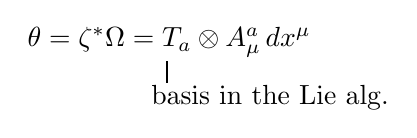
\begin{tikzpicture}[line width=.5pt]
\node[anchor=west,inner sep=0pt] at (0,.7)
  {\(\theta=\zeta^*\Omega=T_a\otimes A_\mu^a\,dx^\mu\)};
\draw (1.78,.46)--(1.78,.19);
\node[anchor=west,inner sep=0pt] at (1.57,0) {basis in the Lie alg.};
\end{tikzpicture}}\endgroup\par
The letter \(T\) is retraced. The stroke underneath marks the label.}
\end{GelfandAdjacentEvidence}
\begin{GelfandAdjacentEvidence}{GELFAND-P000677}{4}

\[
\zeta^{*}\Phi=T_a\otimes F_{\mu\nu}^a\,dx^\mu\wedge dx^\nu.
\]
\Unclear{GELFAND-P000677}{curvature-formula}{The symbol before the star is the same sign rendered as \(\zeta\).}
\end{GelfandAdjacentEvidence}
\begin{GelfandAdjacentEvidence}{GELFAND-P000677}{5}


\underline{Projection of the eq.:}
\[
\underline{\delta_M(\zeta^{*}\varphi)+\ast^{-1}
[\theta,\ast\zeta^{*}\Phi]=0.}
\]
\Unclear{GELFAND-P000677}{projection-formula}{The first section symbol is followed by \(\varphi\), the second by \(\Phi\). Two small strokes lie at the lower edge of the bracket.}
\end{GelfandAdjacentEvidence}
\begin{GelfandAdjacentEvidence}{GELFAND-P000677}{6}

\(\delta_M\) --- the op. \(\delta\) on the base.

Direct calc. shows this is the same eq.

It is the same eq. if the group has a 2-sided inv. metric.

\uwave{The vacuum Einstein eqs. are here} (\underline{Ricci tensor}\(=0\))

\(G=\) \uwave{affine transformations of} \(\mathbb R^4\)

(eq. in the bundle of aff. frames)

On the aff. frames there are 2 natural connections ind. by the base metric.

On the class of Cartan connections ind. by metrics.

\Unclear{GELFAND-P000677}{connection-paragraph-mark}{The retraced sign on the left resembles a 4.}
\end{GelfandAdjacentEvidence}
\begin{GelfandAdjacentEvidence}{GELFAND-P000677}{7}

There is a unique conn.
\Incomplete{GELFAND-P000677}{connection-cancel}{Crossed-out mark before \(\bar\Omega\).}
\end{GelfandAdjacentEvidence}
\begin{GelfandAdjacentEvidence}{GELFAND-P000677}{8}

\(\bar\Omega\) in the bundle of aff. frames, such that
\[
\text{if}\quad
\underset{\text{lin.}}{L}\overset{i}{\hookrightarrow}
\underset{\text{aff.}}{AL}\qquad
i^*\bar\Omega=(\Omega^g,\chi);
\]
\(\chi\) --- displacement form

(nat. form with values in \(\mathbb R^4\) on the bundle of lin. frames)
\SourceFigure{GELFAND-P000677}{shift-insertion}{%
\par\smallskip
\begingroup\color{black}\GelfandFitDiagram{\begin{tikzpicture}[line width=.5pt]
\draw (0,.51)--(.85,.55) (0,.57)--(.86,.50);
\node[draw,ellipse,inner sep=2pt] (note) at (1.08,0) {lin.};
\draw (note.north west) to[out=72,in=240] (1.17,.63);
\end{tikzpicture}}\endgroup\par
The outlined “lin.” below points to the position before “frames”. The earlier writing is crossed out.}
\end{GelfandAdjacentEvidence}
\begin{GelfandAdjacentEvidence}{GELFAND-P000677}{9}


\(\Omega^g\) --- metric connection

\noindent\rule{14mm}{.45pt}\enspace\(\cdot\)\enspace\rule{15mm}{.45pt}

def. of a Cartan connection --- see Bishop and Crittenden.

on these connections \(\underline{H\delta\varphi=0}\) --- \uwave{Einstein’s equation}.
(1st order in the connection!! --- unlike for general Yang–Mills fields)

2nd order eqs. ---
\Incomplete{GELFAND-P000677}{consequence-cancel}{Crossed-out writing before “consequence”.}
\end{GelfandAdjacentEvidence}
\begin{GelfandAdjacentEvidence}{GELFAND-P000677}{10}

a consequence of the 1st order eqs.

\SourceFigure{GELFAND-P000677}{ricci-diagram}{%
\par\smallskip
\begingroup\color{black}\GelfandFitDiagram{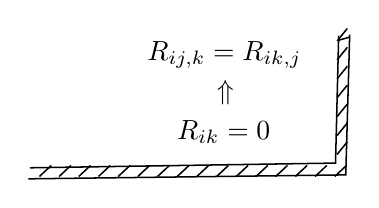
\begin{tikzpicture}[line width=.55pt]
\node at (.39,1.47) {\(R_{ij,k}=R_{ik,j}\)};
\node at (.40,.99) {\(\Uparrow\)};
\node at (.38,.49) {\(R_{ik}=0\)};
\draw (-2.08,.04)--(1.80,.10)--(1.84,1.72);
\draw (-2.10,-.10)--(1.93,-.05)--(1.98,1.73);
\draw (1.84,1.66)--(1.98,1.70);
\foreach \x in {-1.96,-1.71,...,1.79}
  \draw (\x,-.07)--++(.15,.14);
\foreach \y in {.21,.45,...,1.65}
  \draw (1.82,\y)--++(.13,.16);
\end{tikzpicture}}\endgroup\par
The double arrow points up. A hatched corner runs along the bottom and right.}
\end{GelfandAdjacentEvidence}



\Needspace{7\baselineskip}
\begin{GelfandAdjacentEvidence}{GELFAND-P000678}{1}
\SourcePage{GELFAND-P000678}{unlabelled}
\underline{Gelfand seminar.}

\underline{I. N. Bernstein.}

\underline{Kostant.}
\[
\begin{aligned}
\underline{\varphi(x)=\prod_{n=1}^{\infty}(1-x^n)
   =(1-x)(1-x^2)(1-x^3)\times\ldots}\\
=\sum_{n=-\infty}^{\infty}(-1)^n x^{(3n^2+n)/2}.
\end{aligned}
\]
\Unclear{GELFAND-P000678}{euler-product}{The retraced lower limit of the product reads \(n=1\).}
\end{GelfandAdjacentEvidence}
\begin{GelfandAdjacentEvidence}{GELFAND-P000678}{2}

\Unclear{GELFAND-P000678}{euler-factor-mark}{The dark mark between the third factor and the ellipsis resembles \(\times\).}
\end{GelfandAdjacentEvidence}
\begin{GelfandAdjacentEvidence}{GELFAND-P000678}{3}

\SourceFigure{GELFAND-P000678}{euler-arrow}{%
\par\smallskip
\begingroup\color{black}\GelfandFitDiagram{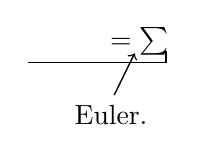
\begin{tikzpicture}[line width=.5pt]
\node[inner sep=0pt] at (1.36,.78) {\(=\sum\)};
\draw (-.05,.51)--(1.7,.51)--(1.7,.66);
\draw[->] (1.04,.10)--(1.30,.63);
\node[inner sep=0pt] at (1.00,-.15) {\uwave{Euler}.};
\end{tikzpicture}}\endgroup\par
The arrow from the name points to the equality with the sum.}
\end{GelfandAdjacentEvidence}
\begin{GelfandAdjacentEvidence}{GELFAND-P000678}{4}


\underline{Jacobi:}
\[
\varphi(x)^3=\sum_{n=0}^{\infty}(-1)^n(2n+1)x^{n(n+1)/2}
\]
(from the \(\Theta\)-function).
\Unclear{GELFAND-P000678}{jacobi-theta-case}{The oval crossed by a horizontal stroke is rendered as uppercase \(\Theta\).}
\end{GelfandAdjacentEvidence}
\begin{GelfandAdjacentEvidence}{GELFAND-P000678}{5}


Others have since been found (Dyson et al.)

\uwave{Macdonald found a group-theoretic basis.}

It is easy to check that
\[
\varphi(x)^{-1}=\sum p(n)x^n,
\]
\(p(n)\) --- number of partitions of \(n\) into a sum of nonnegative summands

\[
x\varphi(x)^{24}=\sum\tau(n)x^n,
\]
\(\tau(n)\) --- Ramanujan’s function

this is its definition

\(\tau(n)\) has a combinatorial definition

\Incomplete{GELFAND-P000678}{dedekind-cancel}{Crossed-out writing above the line beginning “via”.}
\end{GelfandAdjacentEvidence}
\begin{GelfandAdjacentEvidence}{GELFAND-P000678}{6}

(via Dedekind’s \(\Theta\)-fn.)
\Unclear{GELFAND-P000678}{dedekind-theta-case}{The glyph before “fn.” is rendered as \(\Theta\), as in the line about Jacobi’s formula.}
\end{GelfandAdjacentEvidence}
\begin{GelfandAdjacentEvidence}{GELFAND-P000678}{7}


one can write
\[
\varphi(x)^k,\quad \text{where }k\text{ --- dimension of the Lie group (semisimple)}
\]
\SourceFigure{GELFAND-P000678}{step-table}{%
\par\smallskip
\begingroup\color{black}\GelfandFitDiagram{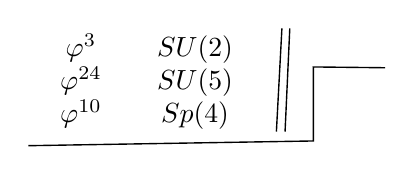
\begin{tikzpicture}[line width=.5pt]
\node[anchor=west,inner sep=0pt] at (.22,.80)
  {\(\begin{array}{c@{\qquad}c}
     \varphi^3&SU(2)\\
     \varphi^{24}&SU(5)\\
     \varphi^{10}&Sp(4)
   \end{array}\)};
\draw (3.15,.18)--(3.22,1.49) (3.26,.18)--(3.32,1.49);
\draw (0,0)--(3.62,.06)--(3.62,1.00)--(4.53,.99);
\end{tikzpicture}}\endgroup\par
A double rule stands to the right of the three rows. The stepped line below rises to the next paragraph.}
\end{GelfandAdjacentEvidence}
\begin{GelfandAdjacentEvidence}{GELFAND-P000678}{8}


\dashuline{Macdonald}: writes out the formula explicitly.

Let there be a compact semisimple group
\Incomplete{GELFAND-P000678}{group-cancellations}{Two crossed-out pieces of writing between “group” and its symbol.}
\end{GelfandAdjacentEvidence}
\begin{GelfandAdjacentEvidence}{GELFAND-P000678}{9}

\(G\)

\(g\) --- its Lie algebra, on \(g\) there is the Killing form \(B\)

\(\Delta\) --- the Laplace operator on
\Incomplete{GELFAND-P000678}{laplace-cancellations}{Two crossed-out pieces of writing after “on”.}
\end{GelfandAdjacentEvidence}
\begin{GelfandAdjacentEvidence}{GELFAND-P000678}{10}

\(G\)

\(X_1,\ldots,X_k\) --- orthonorm. basis in \(g\).

In the enveloping algebra
\SourceFigure{GELFAND-P000678}{enveloping-insertion}{%
\par\smallskip
\begingroup\color{black}\GelfandFitDiagram{\begin{tikzpicture}[line width=.5pt]
\node[anchor=west,inner sep=0pt] (word) at (0,.73) {algebra};
\node[draw,ellipse,inner sep=1.7pt] (note) at (1.12,0) {\(U(g)\)};
\draw (note.north west) to[out=52,in=-120] (word.south east);
\draw (note.north east) to[out=118,in=-60] (word.south east);
\end{tikzpicture}}\endgroup\par
\(U(g)\) is outlined below “algebra”.}
\end{GelfandAdjacentEvidence}
\begin{GelfandAdjacentEvidence}{GELFAND-P000678}{11}

consider the element
\Incomplete{GELFAND-P000678}{enveloping-cancel}{Crossed-out formula before the element.}
\end{GelfandAdjacentEvidence}

\(\Delta=\sum X_i^2\). it is 2-sided invariant.


\Needspace{7\baselineskip}
\begin{GelfandAdjacentEvidence}{GELFAND-P000679}{1}
\SourcePage{GELFAND-P000679}{unlabelled}
\[
\varphi(x)^k=\sum_{\text{irred. reps. }V}
c_V\cdot\dim V\cdot x^{\left.\Delta\right|_V}
\]
\Incomplete{GELFAND-P000679}{top-exponent-cancellation}{Crossed-out writing in the exponent before \(\Delta|_V\).}
\end{GelfandAdjacentEvidence}
\begin{GelfandAdjacentEvidence}{GELFAND-P000679}{2}


(\(\left.\Delta\right|_V\) is a multiple of the identity;
eigenvalue \(\left.\Delta\right|_V\).
\SourceFigure{GELFAND-P000679}{irreducible-insertion}{%
\par\smallskip
\begingroup\color{black}\GelfandFitDiagram{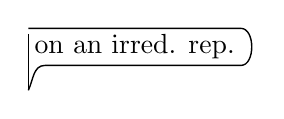
\begin{tikzpicture}[line width=.5pt]
\node[inner sep=2pt] (note) {on an irred. rep.};
\draw (note.north west)--(note.north east) to[out=0,in=0] (note.south east)
      --([xshift=6pt]note.south west) to[out=180,in=65] ([yshift=-9pt]note.south west);
\draw ([yshift=-2pt]note.north west)--([yshift=-9pt]note.south west);
\end{tikzpicture}}\endgroup\par
The insertion above the line points after \(\Delta|_V\).}
\end{GelfandAdjacentEvidence}
\begin{GelfandAdjacentEvidence}{GELFAND-P000679}{3}


\sout{Hence} The asymptotics depend on the dimension.
\Unclear{GELFAND-P000679}{top-word-cancellation}{The crossed-out word tentatively reads “Отсюда” (hence).}
\end{GelfandAdjacentEvidence}
\begin{GelfandAdjacentEvidence}{GELFAND-P000679}{4}


Groups vary, and so do the formulas.
\[
c_V=\chi_V(a),\qquad
\text{where }\underset{\text{a certain element}}{a\in G}
\]

\sout{For the series.} For \(SU(n)\) there is a unique reg. element.
(class of conjugate elements;) i.e., one whose eigenvalues are distinct and whose
\Incomplete{GELFAND-P000679}{su-n-power-cancellation}{Crossed-out mark before the \(n\)th power.}
\end{GelfandAdjacentEvidence}
\begin{GelfandAdjacentEvidence}{GELFAND-P000679}{5}

\(n\)th power is scalar.

\Incomplete{GELFAND-P000679}{matrix-left-cancellation}{Crossed-out mark left of the matrix bracket.}
\end{GelfandAdjacentEvidence}
\begin{GelfandAdjacentEvidence}{GELFAND-P000679}{6}

\[
\begin{pmatrix}
 \xi&&&&0\\
 &\xi^2&&&\\
 &&\xi^3&&\\
 &&&\ddots&\\
 0&&&&\xi^n
\end{pmatrix}c,\qquad c\quad \text{\uwave{chosen so that} }\det=1.
\]

Consider the \(\zeta\)-function of the Laplace op.

\uwave{V. Kac} --- proof \underline{via}
\(\underline{\infty}\)-dimensional Lie algebras.

Consider \(-\Delta+\dfrac{\dim g}{24}\) and set
\[
\zeta(s)\underset{\mathrm{def}}{=}
\left.\left(-\Delta+\frac{\dim g}{24}\right)^{-s}\right|_a
\]
\Incomplete{GELFAND-P000679}{zeta-definition-cancellation}{Crossed-out writing after the defining equality.}
\end{GelfandAdjacentEvidence}
\begin{GelfandAdjacentEvidence}{GELFAND-P000679}{7}

(op. of convolution with a fn.,
\Unclear{GELFAND-P000679}{kernel-comment-cancellations}{Two crossed-out passages. The second tentatively contains “ядро” (kernel).}
\end{GelfandAdjacentEvidence}
\begin{GelfandAdjacentEvidence}{GELFAND-P000679}{8}

constant on classes of conj. elements,
its value is taken at \(a\))

\(K(x,y)\) --- kernel. In fact \(K(xy^{-1})\)

About \sout{\(\zeta(s)\)} one can say something
\Unclear{GELFAND-P000679}{pro-zeta-cancellation}{The crossed-out expression tentatively reads \(\zeta(s)\).}
\end{GelfandAdjacentEvidence}
\begin{GelfandAdjacentEvidence}{GELFAND-P000679}{9}


\underline{Theorem.}
\SourceFigure{GELFAND-P000679}{theorem-bracket}{%
\par\smallskip
\begingroup\color{black}\GelfandFitDiagram{\begin{tikzpicture}[line width=.5pt]
\node[inner sep=2pt] (formula) {\(\zeta(s)=\zeta\left(\dfrac{\dim g}{2}-s\right)\)};
\draw ([yshift=3pt]formula.south west)--(formula.south west)--
      (formula.south east)--([yshift=3pt]formula.south east);
\end{tikzpicture}}\endgroup\par
The line below the formula has upturned ends.}
\end{GelfandAdjacentEvidence}
\begin{GelfandAdjacentEvidence}{GELFAND-P000679}{10}

\Unclear{GELFAND-P000679}{dimension-letter}{The letter after \(\dim\) is rendered as \(g\) in all three formulas.}
\end{GelfandAdjacentEvidence}
\begin{GelfandAdjacentEvidence}{GELFAND-P000679}{11}


The theorem is equiv. to an
\Incomplete{GELFAND-P000679}{theorem-word-cancellation}{Crossed-out word after “equiv.”.}
\end{GelfandAdjacentEvidence}
\begin{GelfandAdjacentEvidence}{GELFAND-P000679}{12}

identity for \(\varphi(x)^k\).

There are also \(\varphi^{39},\ \varphi^{45}\qquad\text{Van Esh}\)
\Unclear{GELFAND-P000679}{van-esh-name}{The name is written in Latin script as “Van Esh”.}
\end{GelfandAdjacentEvidence}
\begin{GelfandAdjacentEvidence}{GELFAND-P000679}{13}


see \underline{Garland, Lepowsky}, Inv. math., 34 (1976), 37--76

\noindent\rule{13mm}{.45pt}\enspace\(\cdot\)\enspace\rule{14mm}{.45pt}

\Incomplete{GELFAND-P000679}{olshanetsky-preceding-cancellation}{The underlined word before the surname is crossed out.}
\end{GelfandAdjacentEvidence}
\begin{GelfandAdjacentEvidence}{GELFAND-P000679}{14}

\underline{Olshanetsky.}

\(\Delta^0\) --- rad. part of the Laplace op.
\SourceFigure{GELFAND-P000679}{symmetric-space-insertion}{%
\par\smallskip
\begingroup\color{black}\GelfandFitDiagram{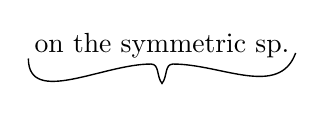
\begin{tikzpicture}[line width=.5pt]
\node[inner sep=2pt] (note) {on the symmetric sp.};
\draw ([yshift=2pt]note.south west) to[out=-90,in=180]
      ([xshift=-4pt]note.south) to[out=0,in=130] ([yshift=-7pt]note.south)
      to[out=50,in=180] ([xshift=4pt]note.south) to[out=0,in=-110]
      ([yshift=4pt]note.south east);
\end{tikzpicture}}\endgroup\par
The insertion stands above the line after “Laplace”.}
\end{GelfandAdjacentEvidence}
\begin{GelfandAdjacentEvidence}{GELFAND-P000679}{15}

It is written in the form
\[
\longrightarrow\frac12\frac{\partial^2}{\partial t_k^2}
 +U(t_1,\ldots,t_n)
\]
\[
U=g\sum_{k>\ell}\frac1{\sin^2(t_k-t_\ell)}
\]
And there is a complete system of observables in the quantum sense.

\noindent\rule{14mm}{.45pt}\enspace\(\cdot\)\enspace\rule{15mm}{.45pt}

\underline{\underline{I. Bernstein.}}\qquad
\underline{\underline{on V. G. Kac’s work.}}

\underline{Construction of a Lie algebra from a Cartan matrix.}

\(\underset{n\times n}{(a_{ij})}\) --- matrix with integer entries, for which
\[
a_{ij}<0\quad\text{when }i\ne j
\qquad\Vert\qquad
\begin{aligned}
a_{ii}&=2,\\
a_{ij}\ne0&\Rightarrow a_{ji}\ne0
\end{aligned}
\]
(zeros occur symmetrically)
\Unclear{GELFAND-P000679}{cartan-strict-inequality}{The sign between \(a_{ij}\) and zero is written without a lower stroke.}
\end{GelfandAdjacentEvidence}
\begin{GelfandAdjacentEvidence}{GELFAND-P000679}{16}

\Unclear{GELFAND-P000679}{cartan-zero-comment}{The ending of the last word runs into the bracket. It tentatively reads “симметрично” (symmetrically).}
\end{GelfandAdjacentEvidence}



\Needspace{7\baselineskip}
\begin{GelfandAdjacentEvidence}{GELFAND-P000680}{1}
\SourcePage{GELFAND-P000680}{unlabelled}
\SourceFigure{GELFAND-P000680}{left-rule}{%
\begingroup\color{black}\GelfandFitDiagram{\begin{tikzpicture}[line width=.5pt]
\draw (0,0)--(0,.85)--(.12,.85);
\end{tikzpicture}}\endgroup\enspace Vertical rule along the left margin.}
\end{GelfandAdjacentEvidence}
\begin{GelfandAdjacentEvidence}{GELFAND-P000680}{2}


A Lie alg. is constructed from such a matrix.

Consider \(h_i,e_i,f_i\), free generators (\(n\) of them), and write the relations

\SourceFigure{GELFAND-P000680}{relation-outline}{%
\begingroup\color{black}\GelfandFitDiagram{\begin{tikzpicture}[line width=.5pt]
\node[inner sep=3pt] (relations) {\(\begin{aligned}
\relax[h_i,e_j]&=-a_{ij}e_j,\\
[h_i,f_j]&=+a_{ij}f_j.\\
[h_i,h_j]&=0,\\
[e_i,f_i]&=h_i\cdot\delta_{ij}
\end{aligned}\)};
\draw (relations.south west)--(relations.south east)--(relations.north east);
\end{tikzpicture}}\endgroup\par
The outline runs below and to the right of the relations.}
\end{GelfandAdjacentEvidence}
\begin{GelfandAdjacentEvidence}{GELFAND-P000680}{3}

\Unclear{GELFAND-P000680}{generator-signs}{The first line has a minus sign before \(a_{ij}\), and the second has a plus sign.}
\end{GelfandAdjacentEvidence}
\begin{GelfandAdjacentEvidence}{GELFAND-P000680}{4}

\Unclear{GELFAND-P000680}{ef-generator-indices}{The last line appears to give both \(e\) and \(f\) the same subscript \(i\).}
\end{GelfandAdjacentEvidence}
\begin{GelfandAdjacentEvidence}{GELFAND-P000680}{5}


(take the quotient of the free alg. by these relations)
and take the quotient of this alg. by the \(\max\) normal subalgebra
[Inserted at left above the formula: and further rels.]
\Unclear{GELFAND-P000680}{relations-insertion}{The last word is abbreviated in the manuscript as “соотнош.” (relations).}
\end{GelfandAdjacentEvidence}
\begin{GelfandAdjacentEvidence}{GELFAND-P000680}{6}

\[
\underbrace{[e_i[e_i[e_i\ldots[e_i}_{-a_{ij}+1},e_j]]\mathord{..}]=0
\]
\Unclear{GELFAND-P000680}{nested-bracket-count}{The underbrace ends before the comma. After \(e_j\) there are two closing brackets, two dots and a further closing bracket.}
\end{GelfandAdjacentEvidence}
\begin{GelfandAdjacentEvidence}{GELFAND-P000680}{7}


For certain matrices, classical groups arise.
\(SU(2)\qquad e_+,h_+,f_+\qquad\text{matrix }1\times1\Vert(2)\)
\Unclear{GELFAND-P000680}{su-two-basis-indices}{All three letters have a plus subscript.}
\end{GelfandAdjacentEvidence}
\begin{GelfandAdjacentEvidence}{GELFAND-P000680}{8}

\[
[h,e]=2e,\qquad[h,f]=-2f,\qquad[e,f]=h,
\]
\(SU(3)\) is obtained for the matrix \(\begin{pmatrix}2&-1\\-1&2\end{pmatrix}\).

On \underline{roots}: \underline{Serre} “Lie Groups and Lie Algebras” ---
read only this section.

If \(a_{ij}=a_{ji}\), then the following holds:

The group is finite-dimensional \(\Leftrightarrow\) the matrix is positive definite.
\[
\begin{pmatrix}
2&-1&-1\\
-1&2&-1\\
-1&-1&2
\end{pmatrix}
\quad\text{--- infinite-dimensional extension of }SU(3).
\]
\underline{V. G. Kac.}\ : the quotient of this alg. by its one-dimensional centre is
\[
SU(3)\otimes\mathbb C[x,x^{-1}].
\]
\[
[x^kg,x^\ell g']=x^{k+\ell}[g,g'].
\]
all the non-strictly def. ones are obtained this way.
\Unclear{GELFAND-P000680}{loop-wording}{The two abbreviated words read “нестрог. опред.” (non-strictly definite).}
\end{GelfandAdjacentEvidence}


\uwave{Happy New Year!}


\Needspace{7\baselineskip}
\begin{GelfandAdjacentEvidence}{GELFAND-P000681}{1}
\SourcePage{GELFAND-P000681}{unlabelled}

\underline{14/II-77.}\qquad\underline{Gelfand Sem.}

\underline{Yu. I. Manin.}

\dashuline{Calogero}: boomeron:
\SourceFigure{GELFAND-P000681}{upper-wave-sketch}{%
\begingroup\color{black}\GelfandFitDiagram{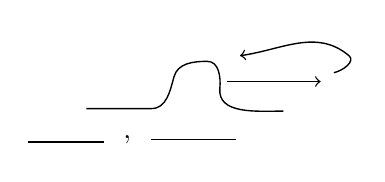
\begin{tikzpicture}[x=8mm,y=8mm,line width=.5pt]
\draw (0,.15) to[out=0,in=180] (1.03,.15)
  to[out=0,in=-105] (1.39,.65) to[out=75,in=180] (1.92,.9)
  to[out=0,in=85] (2.12,.47) to[out=-95,in=180] (3.13,.11);
\draw[->] (3.93,.72) to[out=12,in=-40] (4.17,.99)
  to[out=140,in=8] (2.44,.99);
\draw[->] (2.24,.58)--(3.72,.58);
\draw (-.92,-.38)--(.28,-.38) (1.03,-.34)--(2.38,-.34);
\node at (.65,-.35) {,};
\end{tikzpicture}}\endgroup\par
The upper arrow hooks down at the right. A gap is visible between the hook and the point of the lower arrow.}
\end{GelfandAdjacentEvidence}
\begin{GelfandAdjacentEvidence}{GELFAND-P000681}{2}

\Unclear{GELFAND-P000681}{boomeron-heading}{The underline under “Calogero” is broken. The next word reads “бумерон” (boomeron).}
\end{GelfandAdjacentEvidence}
\begin{GelfandAdjacentEvidence}{GELFAND-P000681}{3}


Equation of Lax type
\[
\overset{\text{\textcircled{\scriptsize 4}}}{L}_t=
[\overset{\text{\textcircled{\scriptsize 4}}}{L},
 \overset{\text{\textcircled{\scriptsize 2}}}{P}]
\]
\Unclear{GELFAND-P000681}{circled-orders}{A circled 4 stands over each \(L\), and a circled 2 over \(P\).}
\end{GelfandAdjacentEvidence}
\begin{GelfandAdjacentEvidence}{GELFAND-P000681}{4}

\[
L=\partial^4+v\partial^2+w\partial+z,\qquad
\partial=\partial/\partial x.
\]
\[
P=\partial^2+A\partial+u
\]
\(u\) is expressed in terms of \(v,w,z\).
\[
\left\{\begin{aligned}
v_t&=v_{xx}-Av_x-2w_x\\
w_t&=2v_{xxx}+2vv_x-w_{xx}-Aw_x-2z_x\\
z_t&=\tfrac12v_{xxxx}+\tfrac12vv_{xx}+\tfrac12v_xw-z_{xx}-Az_x
\end{aligned}\right.
\]
\Unclear{GELFAND-P000681}{evolution-coefficients}{The first line has no written coefficient before \(v_{xx}\). The second has a 2 before \(vv_x\).}
\end{GelfandAdjacentEvidence}
\begin{GelfandAdjacentEvidence}{GELFAND-P000681}{5}


1-soliton solution
\[
\mu_1=2\frac{\operatorname{ch}2\xi-\cos 2\xi+2\sin\sigma t}
               {\operatorname{ch}2\xi+\cos 2\xi-2\cos\sigma t}
\]
\[
\mu_2=2\frac{\operatorname{sh}2\xi-\sin 2\xi}
               {\operatorname{ch}2\xi+\cos 2\xi-2\cos\sigma t}
\]
\Unclear{GELFAND-P000681}{mu-two-raised-mark}{A thickened mark above and to the right of the factor \(2\), before \(\operatorname{sh}\), may be a crossed-out digit.}
\end{GelfandAdjacentEvidence}
\begin{GelfandAdjacentEvidence}{GELFAND-P000681}{6}

\[
\xi=x+ct\qquad
\begin{aligned}
c&\in\mathbb R\\
\sigma&\in\mathbb R\\
\sigma&\leftrightarrow A\quad\text{(is expressed).}
\end{aligned}
\]
\[
\left\{\begin{aligned}
v&=-4\mu_{2x}\\
\sigma w&=4\mu_2\mu_{2x}+6\mu_{2xx}+4\mu_{1x}\\
z&=.\;.\;.\;.\qquad\text{(inessential)}
\end{aligned}\right.
\]
\Unclear{GELFAND-P000681}{sigma-w}{The left-hand side of the second line reads \(\sigma w\).}
\end{GelfandAdjacentEvidence}
\begin{GelfandAdjacentEvidence}{GELFAND-P000681}{7}


\SourceFigure{GELFAND-P000681}{lower-mu-one-sketch}{%
\begingroup\color{black}\GelfandFitDiagram{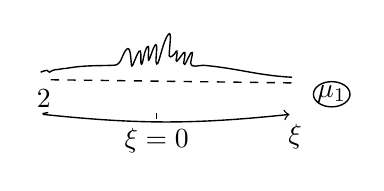
\begin{tikzpicture}[x=8mm,y=8mm,line width=.5pt]
\draw[dashed] (.23,.65)--(4.08,.6);
\node[below] at (.12,.65) {\(2\)};
\draw (.07,.77) to[out=15,in=180] (.17,.8)
  to[out=0,in=200] (.21,.77) to[out=25,in=185] (.3,.81)
  to[out=0,in=180] (.47,.83) to[out=10,in=182] (1.23,.88)
  to[out=0,in=-130] (1.43,1.13) to[out=50,in=95] (1.51,.89)
  to[out=-85,in=-125] (1.63,1.10) to[out=55,in=90] (1.66,.92)
  to[out=-75,in=-125] (1.76,1.17) to[out=55,in=95] (1.78,.98)
  to[out=-90,in=-120] (1.88,1.19) to[out=55,in=90] (1.90,.94)
  to[out=-80,in=-125] (2.09,1.36) to[out=55,in=90] (2.11,1.03)
  to[out=-75,in=-110] (2.22,1.10) to[out=55,in=80] (2.22,.96)
  to[out=-90,in=-135] (2.34,1.08) to[out=45,in=85] (2.34,.91)
  to[out=-80,in=-130] (2.46,1.08) to[out=45,in=85] (2.45,.91)
  to[out=-80,in=180] (2.65,.88) to[out=-5,in=177] (4.06,.69);
\draw[->] (.11,.1) to[out=-6,in=186] (4.02,.1);
\draw (.11,.1) to[out=130,in=210] (.19,.13);
\draw (1.91,.03)--(1.91,.13);
\node[below] at (1.91,.03) {\(\xi=0\)};
\node[below] at (4.11,.10) {\(\xi\)};
\draw (4.69,.42) ellipse (.29 and .20);
\node at (4.69,.42) {\(\mu_1\)};
\end{tikzpicture}}\endgroup\par
At the left end of the axis there is a hook and a set of small illegible marks.}
\end{GelfandAdjacentEvidence}
\begin{GelfandAdjacentEvidence}{GELFAND-P000681}{8}


[To the right of the graph:] every \(\dfrac{2\pi}{\sigma}\) periodically
\Incomplete{GELFAND-P000681}{periodic-comment-cancellation}{A sign or short passage is crossed out at the end of the line.}
\end{GelfandAdjacentEvidence}

it spits
(geyseron, spiton, \(.\;.\;.\;.\))
explosive instability.

\underline{Algebraic method.}

a) construct an aux. stationary eq.
\([L_1,P_1]=0\)\qquad then introduce \(t\).

b)
\[
\left\{\begin{aligned}
L_1\psi&=\lambda\psi\\
P_1\psi&=\mu\psi
\end{aligned}\right.
\qquad
(\lambda,\mu)\in X\quad\text{--- aff. alg. curve}
\]
the case studied was: \underline{\(\dim(\text{space of }\psi)=1\)}.

Krichever did not state it explicitly, but it followed from the constraints.

\underline{Drinfeld} --- did not specify the solution explicitly, but indicated the difficulties.


\Needspace{7\baselineskip}
\begin{GelfandAdjacentEvidence}{GELFAND-P000682}{1}
\SourcePage{GELFAND-P000682}{unlabelled}
\SourceFigure{GELFAND-P000682}{top-fibre-diagram}{%
\begingroup\color{black}\GelfandFitDiagram{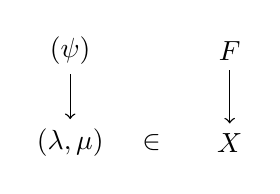
\begin{tikzpicture}[x=9mm,y=9mm,line width=.5pt]
\node (psi) at (0,1.3) {\((\psi)\)};
\node (pair) at (0,0) {\((\lambda,\mu)\)};
\node at (1.15,0) {\(\in\)};
\node (fibre) at (2.25,1.3) {\(F\)};
\node (base) at (2.25,0) {\(X\)};
\draw[->] (psi)--(pair);
\draw[->] (fibre)--(base);
\end{tikzpicture}}\endgroup\par
Both arrows point down. The mark between the lower entries is rendered as \(\in\).}
\end{GelfandAdjacentEvidence}
\begin{GelfandAdjacentEvidence}{GELFAND-P000682}{2}

\Unclear{GELFAND-P000682}{top-map-symbol}{The sign in parentheses reads as \(\psi\). There is an additional fine stroke in its centre.}
\end{GelfandAdjacentEvidence}
\begin{GelfandAdjacentEvidence}{GELFAND-P000682}{3}


The bundle extends to the completion.
\Unclear{GELFAND-P000682}{top-opening-abbreviations}{The middle word is abbreviated. It tentatively reads “продолж.” (extends).}
\end{GelfandAdjacentEvidence}
\begin{GelfandAdjacentEvidence}{GELFAND-P000682}{4}

We obtain a bundle on the curve
\[
t\longrightarrow\text{path on the Jacobian.}
\]
\[
\underset{\text{Moduli of the system;}}{\underline{\underline{r>1}}}
\quad\Rightarrow\quad\text{path in the moduli of bundles.}
\]
Hyperell. curve \(\longrightarrow\) intersection of 2 quadrics in \(\mathbb C^5\).
\Unclear{GELFAND-P000682}{hyperelliptic-ambient}{The space is written \(\mathbb C^5\).}
\end{GelfandAdjacentEvidence}
\begin{GelfandAdjacentEvidence}{GELFAND-P000682}{5}

Analyt. paths?

A soliton is a solution of the nonstationary eq. obtained by taking a curve with one double point with distinct tangents in the stationary eq.

\underline{Notation}. \(k\) --- field of char. 0.
\[
\underset{\text{in the analytic setting,}}{(k=\mathbb R\ \text{or}\ \mathbb C)}
\]
\(\mathcal B\) --- \(k\)-alg.
\[
\left(\begin{aligned}
\mathcal B&=\underset{\text{matrices}}{M_\ell}(\mathcal B_0),\\
\mathcal B_0&=\text{field of rat. }k\text{-anal. }
          \overset{\text{merom.}}{\text{functions}}\ \text{of }
          \begin{matrix}x\\x,t\\x,t,z\end{matrix}
\end{aligned}\right)
\]
\Unclear{GELFAND-P000682}{meromorphic-insertion}{The abbreviation “мером.” (meromorphic) is inserted above the space before “ф-й” (functions) with a curved callout.}
\end{GelfandAdjacentEvidence}
\begin{GelfandAdjacentEvidence}{GELFAND-P000682}{6}


\[
\underset{\text{derivations}}{\partial,\partial_1,\partial_2:\mathcal B\longrightarrow\mathcal B},
\qquad [\partial,\partial_i]=[\partial_i,\partial_j]=0
\]
(in the anal. setting \(\partial=\partial/\partial x\), \(\partial_1=\partial/\partial t\),
\(\partial_2=\partial/\partial z\)).

\(\mathcal B[\partial]\)

\((L,P)\) --- pair of ops. satisfying one of the 3 eqs.
\[
\left\{\begin{aligned}
\relax[L,P]&=0 &&\text{stationary Lax}\\
\partial_1 L&=[L,P] &&\text{nonstationary Lax}\\
\partial_1 L+\partial_2 P&=[L,P] &&\text{Zakh.–Shabat}
\end{aligned}\right.
\]

\textcircled{1}\enspace \underline{Krich.–Drinfeld bimodule \(\mathcal M\)}.
\Unclear{GELFAND-P000682}{circled-section}{A circled 1 stands to the left of the heading.}
\end{GelfandAdjacentEvidence}
\begin{GelfandAdjacentEvidence}{GELFAND-P000682}{7}


\underline{Structures}.

a) \(\mathcal M\) --- \(k\)-lin. space, left \(\mathcal B\)-module, right \(\mathcal O\)-module, where

\(\mathcal O\) --- ring of functions on an aff. curve over \(k\); irreducible over \(\bar k\).

b) distinguished element \(\mathbf 1\in\mathcal M\)

c) increasing filtration
\[
\mathcal M_{-1}\subset\mathcal M_0\subset\mathcal M_1\subset\mathcal M_2\subset\ldots,
\qquad\bigcup_{i=0}^\infty\mathcal M_i=\mathcal M
\]
d) \(\nabla:\mathcal M\longrightarrow\mathcal M\qquad k\)-lin. operator.

\underline{Axioms}.

e) the actions \(\overset{\mathcal B\text{ and }\mathcal O}{\text{are faithful}}\) and commute
\Unclear{GELFAND-P000682}{action-insertion}{“\(\mathcal B\) and \(\mathcal O\)” is inserted above the space after “actions” with a curved callout.}
\end{GelfandAdjacentEvidence}
\begin{GelfandAdjacentEvidence}{GELFAND-P000682}{8}


f) \(\mathcal M_{-1}=0,\qquad \mathcal B\mathcal M_i\subset\mathcal M_i\)

g) \(\mathcal M_i/\mathcal M_{i-1}\) --- free \(\mathcal B\)-module of rank \(1;\qquad \mathcal M_0=\mathcal B\mathbf 1\).

h)
\[
\forall b\in\mathcal B,\ m\in\mathcal M:\quad
\nabla(bm)=(\partial b)m+b\nabla m,
\]
\[
\forall\varphi\in\mathcal O,\qquad
(\nabla m)\varphi=\nabla(m\varphi)
\]
\Unclear{GELFAND-P000682}{bottom-retraced-phi}{The letter in \((\nabla m)\varphi\) is retraced. The two nearby instances support reading it as \(\varphi\).}
\end{GelfandAdjacentEvidence}



\Needspace{7\baselineskip}
\begin{GelfandAdjacentEvidence}{GELFAND-P000683}{1}
\SourcePage{GELFAND-P000683}{unlabelled}

(“nabla” is the name of an old musical instrument of the lyre type).

i)
\[
\begin{aligned}
&\forall i\geq-1,\qquad\nabla\mathcal M_i\subset\mathcal M_{i+1},\\
&\nabla:\mathcal M_i/\mathcal M_{i-1}
   \overset{\sim}{\longrightarrow}\mathcal M_{i+1}/\mathcal M_i
\end{aligned}
\]
\Unclear{GELFAND-P000683}{filtration-lower-bound}{The start of the line reads \(i\geq-1\).}
\end{GelfandAdjacentEvidence}
\begin{GelfandAdjacentEvidence}{GELFAND-P000683}{2}


\textcircled{2}\enspace Construction of the bimodule from a pair \(L,P\in\mathcal B[\partial]\)
with \([L,P]=0\) and \(\bar k[L,P]\) without zero divisors.

Set
\[
\mathcal M=\mathcal B[\partial];\qquad \mathcal O=k[L,P].
\]
--- ring of polys. in \(L\) and \(P\).

action of \(\mathcal B\) --- mult. on the left, action of \(\mathcal O\) --- mult. on the right

\(\mathbf1=\) identity operator
\[
\mathcal M_i=\left\{\sum_{k\leq i}b_k\partial^k\mid b_k\in\mathcal B\right\}.
\qquad
\nabla m=\partial\circ m
\]
The axioms are verified trivially.

\underline{Theorem 1}. If there is a \((\mathcal B,\mathcal O)\)-bimodule
\(\mathcal M\), then it gives an embedding \(i:\mathcal O\longrightarrow\mathcal B[\partial]\),
such that the reverse construction from \(i\) gives \(\mathcal M\).

\(\overline{\underline{\text{Construction}}}\).

a)
\SourceFigure{GELFAND-P000683}{endomorphism-diagram}{%
\begingroup\color{black}\GelfandFitDiagram{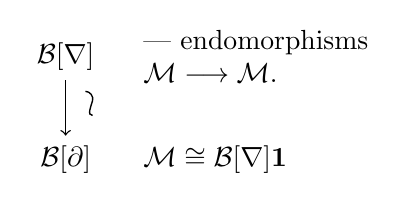
\begin{tikzpicture}[x=9mm,y=9mm,line width=.5pt]
\node (nabla) at (0,1.45) {\(\mathcal B[\nabla]\)};
\node (d) at (0,0) {\(\mathcal B[\partial]\)};
\node[anchor=west,inner sep=1pt,align=left] at (1.05,1.45)
  {--- endomorphisms\\
   \(\mathcal M\longrightarrow\mathcal M\).};
\node[anchor=west,inner sep=1pt] at (1.05,0)
  {\(\mathcal M\cong\mathcal B[\nabla]\mathbf1\)};
\draw[->] (nabla)--(d);
\draw (.28,.96) to[out=0,in=75] (.38,.83)
  to[out=-105,in=180] (.38,.62);
\end{tikzpicture}}\endgroup}
\end{GelfandAdjacentEvidence}
\begin{GelfandAdjacentEvidence}{GELFAND-P000683}{3}

\Unclear{GELFAND-P000683}{construction-vertical-arrow}{A separate vertical wavy stroke stands to the right of the down arrow.}
\end{GelfandAdjacentEvidence}
\begin{GelfandAdjacentEvidence}{GELFAND-P000683}{4}

This step did not use multiplication by \(\mathcal O\).

b)
\SourceFigure{GELFAND-P000683}{embedding-diagram}{%
\begingroup\color{black}\GelfandFitDiagram{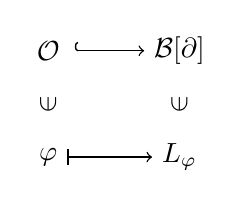
\begin{tikzpicture}[x=9mm,y=9mm,line width=.5pt]
\node (o) at (0,1.5) {\(\mathcal O\)};
\node (d) at (1.85,1.5) {\(\mathcal B[\partial]\)};
\node (phi) at (0,0) {\(\varphi\)};
\node (l) at (1.85,0) {\(L_\varphi\)};
\coordinate (hook) at ([xshift=3pt]o.east);
\draw[->] (hook)--(d);
\draw (hook) to[out=180,in=180] ([yshift=3pt]hook);
\draw[|->] (phi)--(l);
\node[rotate=90,inner sep=0pt] at (0,.75) {\(\in\)};
\node[rotate=90,inner sep=0pt] at (1.85,.75) {\(\in\)};
\end{tikzpicture}}\endgroup\par
such that \(L_\varphi\mathbf1=\mathbf1\varphi\).
\par
(this determines \(L_\varphi\)).}
\end{GelfandAdjacentEvidence}
\begin{GelfandAdjacentEvidence}{GELFAND-P000683}{5}


\underline{Theorem 2}. Let there be an \((\mathcal O,\mathcal B)\)-bimodule
\(\mathcal M\) and a deriv. \(\partial_1:\mathcal B\longrightarrow\mathcal B\)
(in the anal. setting \(\partial/\partial t\)), and suppose there is also
\(\nabla_1:\mathcal M\longrightarrow\mathcal M\)
\Unclear{GELFAND-P000683}{theorem-two-module-order}{Theorem 2 writes \(\mathcal O\) first and then \(\mathcal B\).}
\end{GelfandAdjacentEvidence}
\begin{GelfandAdjacentEvidence}{GELFAND-P000683}{6}

\[
\left\{\begin{aligned}
\nabla_1(bm)&=\partial_1b+\nabla_1m\\
\nabla_1(m\varphi)&=(\nabla_1m)\varphi\\
[\nabla_1,\nabla]&=0
\end{aligned}\right.
\]
\Unclear{GELFAND-P000683}{theorem-two-first-relation}{The right-hand side shows \(\partial_1b\) and \(\nabla_1m\), with a plus sign between them.}
\end{GelfandAdjacentEvidence}
\begin{GelfandAdjacentEvidence}{GELFAND-P000683}{7}

\[
[\mathcal M,\nabla_1]\longrightarrow\text{family of solns. of nonstationary Lax eqs.}
\]
\[
\begin{gathered}
\nabla_1\mathbf1=P\mathbf1,\qquad P\in B[\partial].\\
\mathbf1\varphi=L_\varphi\mathbf1
\end{gathered}
\]
Then
\SourceFigure{GELFAND-P000683}{bottom-lax-outline}{%
\begingroup\color{black}\GelfandFitDiagram{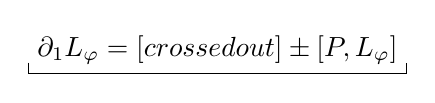
\begin{tikzpicture}[line width=.5pt]
\node[inner sep=3pt] (eq)
 {\(\partial_1L_\varphi=\text{[crossed out]}\pm[P,L_\varphi]\)};
\draw ([yshift=4pt]eq.south west)--(eq.south west)--(eq.south east)
      --([yshift=4pt]eq.south east);
\end{tikzpicture}}\endgroup}
\end{GelfandAdjacentEvidence}
\begin{GelfandAdjacentEvidence}{GELFAND-P000683}{8}

\Incomplete{GELFAND-P000683}{bottom-cancelled-symbol}{A sign is crossed out between the equality sign and \(\pm\).}
\end{GelfandAdjacentEvidence}
\begin{GelfandAdjacentEvidence}{GELFAND-P000683}{9}

\SourceFigure{GELFAND-P000683}{fixed-p-callout}{%
\begingroup\color{black}\GelfandFitDiagram{\begin{tikzpicture}[line width=.5pt]
\draw (0,0)--(0,-.85) (.08,0)--(.08,-.85);
\node[anchor=north west,align=left,inner sep=0pt] at (.22,.06)
  {Here \(P\) is fixed\\and \(L\) varies.};
\end{tikzpicture}}\endgroup}
\end{GelfandAdjacentEvidence}



\Needspace{7\baselineskip}
\begin{GelfandAdjacentEvidence}{GELFAND-P000684}{1}
\SourcePage{GELFAND-P000684}{unlabelled}

\underline{Theorem} 3. A module is given \(\mathcal M\) \uwave{with no mention of} \(\mathcal O\).
\Unclear{GELFAND-P000684}{without-o-wavy-underline}{The wavy underline under “with no mention of” ends before \(\mathcal O\).}
\end{GelfandAdjacentEvidence}
\begin{GelfandAdjacentEvidence}{GELFAND-P000684}{2}


\(\nabla,\nabla_1,\nabla_2\) commute pairwise. Then we obtain solns. of the Zakh.–Shabat eqs.:
\[
\begin{gathered}
\nabla_1\mathbf1=P\mathbf1\\
\nabla_2\mathbf1=L\mathbf1\\
\partial_2P+\partial_1L=\pm[L,P].
\end{gathered}
\]
\Unclear{GELFAND-P000684}{zakharov-shabat-signs}{There is a plus sign between the two derivatives and a \(\pm\) before the commutator.}
\end{GelfandAdjacentEvidence}
\begin{GelfandAdjacentEvidence}{GELFAND-P000684}{3}


Next time \underline{Duistermaat}.
\Unclear{GELFAND-P000684}{duistermaat-name}{The underlined surname is written “Дюйстермаат” (Duistermaat).}
\end{GelfandAdjacentEvidence}
\begin{GelfandAdjacentEvidence}{GELFAND-P000684}{4}


\SourceFigure{GELFAND-P000684}{closing-separator}{%
\begingroup\color{black}\GelfandFitDiagram{\begin{tikzpicture}[line width=.5pt]
\draw (0,0) to[out=135,in=210] (.13,.035)--(1.46,.035);
\fill (1.83,.035) circle (.7pt);
\draw (2.32,.045)--(4.13,.10);
\end{tikzpicture}}\endgroup\par
There is a small hook at the left end of the shorter rule. A dot separates the two rules.}
\end{GelfandAdjacentEvidence}



\Needspace{7\baselineskip}
\begin{GelfandAdjacentEvidence}{GELFAND-P000685}{1}
\SourcePage{GELFAND-P000685}{unlabelled}

\underline{21/II-77}\qquad \underline{Gelfand Sem.}

\underline{Duistermaat.}
\Unclear{GELFAND-P000685}{name-spelling}{The surname is written “Дейстермаат” here.}
\end{GelfandAdjacentEvidence}
\begin{GelfandAdjacentEvidence}{GELFAND-P000685}{2}


\underline{On the Morse index.}

\(I(\gamma)\) --- functional, \(\gamma\) --- curve in \(\mathbb R^n\),
\sout{\(\gamma\in H^1\) (Sobolev sp.)}
\Unclear{GELFAND-P000685}{crossed-sobolev}{The line crosses out \(\gamma\in H^1\) and the parenthetical gloss.}
\end{GelfandAdjacentEvidence}
\begin{GelfandAdjacentEvidence}{GELFAND-P000685}{3}

\[
I(\gamma)=\int_0^T f(\gamma(t),\dot\gamma(t))\,dt
\]
Variational problem.
\[
\gamma\in\text{space of curves such thet }(\gamma(0),\gamma(T))\in R
\]
\Unclear{GELFAND-P000685}{original-english}{The line is in English in the manuscript. The word after “such” tentatively reads “thet”.}
\end{GelfandAdjacentEvidence}
\begin{GelfandAdjacentEvidence}{GELFAND-P000685}{4}


\(R\) --- subset of \(\mathbb R^n\times\mathbb R^n\).

Examples; a) \(R=(0,0)\in\mathbb R^n\times\mathbb R^n\) --- fixed endpoints

b) \(R=\{(x,x)\}\quad\text{---}\quad\gamma(0)=\gamma(T)\) --- periodic condition
\Unclear{GELFAND-P000685}{periodic-separator}{The thick horizontal mark between the formulas is rendered as a dash.}
\end{GelfandAdjacentEvidence}


Extremal --- critical point in \(H^1\).
\[
\begin{aligned}
\text{If }&\frac{\partial^2 f}{\partial\dot\gamma^2}>0,
&\text{then }\operatorname{ind}\frac{\partial^2 I}{\partial\gamma^2}&<\infty\\
&\text{(positive def.)}
&\text{(finitely many neg. squares)}&
\end{aligned}
\]


\Needspace{7\baselineskip}
\begin{GelfandAdjacentEvidence}{GELFAND-P000686}{1}
\SourcePage{GELFAND-P000686}{unlabelled}
\[
\operatorname{ind}\frac{\partial^2 I}{\partial\gamma^2}
=\text{Morse index for the boundary cond.}=\operatorname{ind}_R(\gamma).
\]
There will be a formula for the Morse index in terms of the Arnold index of a curve in the Lagr. set.

\underline{Theorem.}
\[
\text{Morse }\operatorname{index}_R(\gamma)
=\operatorname{ind}(\varphi)+i(I,\rho,\varphi(T))
  +\dim\pi(\rho\cap I)-2n.
\]
\Unclear{GELFAND-P000686}{index-theorem-tail}{The right-hand side reads \(i(I,\rho,\varphi(T))\) and \(\dim\pi(\rho\cap I)-2n\).}
\end{GelfandAdjacentEvidence}
\begin{GelfandAdjacentEvidence}{GELFAND-P000686}{2}


\noindent Eq. for stat. curves (Euler–Lagrange)
\(\underset{\text{Legendre tr.}}{\longrightarrow}\)
Hamilton eq.
\[
(\gamma,\dot\gamma)\underset{\text{Legendre transform}}{\mapsto}
\]

The Hamilton eq. determines a flow of sympl. transformations.

Consider the eq. in variations along the extremal. We obtain a 1-param. family of lin. symplectic transformations.

\(\Phi(t)=\) derivative of the Hamiltonian flow along the extremal curve

this is a lin. transformation:
\[
\underset{\substack{\text{phase}\\\text{space}}}{\mathbb R_\sigma^{2n}}
\longrightarrow \mathbb R_\sigma^{2n}
\]
\Unclear{GELFAND-P000686}{flow-domain-subscript}{The first \(\mathbb R^{2n}\) has a heavily retraced subscript, tentatively read as \(\sigma\).}
\end{GelfandAdjacentEvidence}
\begin{GelfandAdjacentEvidence}{GELFAND-P000686}{3}

\Unclear{GELFAND-P000686}{flow-codomain-subscript}{The second \(\mathbb R^{2n}\) also has a heavily retraced subscript, tentatively read as \(\sigma\).}
\end{GelfandAdjacentEvidence}
\begin{GelfandAdjacentEvidence}{GELFAND-P000686}{4}

\[
\varphi(t)=\operatorname{graph}\varphi(t)\subset
\underline{\mathbb R_\sigma^{2n}\times\mathbb R_{-\sigma}^{2n}}
\qquad \text{(sympl. structure --- difference)}
\]
\Unclear{GELFAND-P000686}{graph-letter}{The letter after “graph” looks lowercase and is transcribed as \(\varphi\).}
\end{GelfandAdjacentEvidence}
\begin{GelfandAdjacentEvidence}{GELFAND-P000686}{5}

\[
\Phi(t)^*\sigma=\sigma.\qquad t\ \text{fixed.}
\]
\[
\Updownarrow
\]
\SourceFigure{GELFAND-P000686}{pullback-letter}{%
\begingroup\color{black}\GelfandFitDiagram{\begin{tikzpicture}[line width=.5pt]
\node[inner sep=3pt] (eq) {\(\sigma-\varphi(t)^*\sigma=0\)};
\draw ([yshift=4pt]eq.south west)--(eq.south west)--(eq.south east)
     --([yshift=4pt]eq.south east);
\end{tikzpicture}}\endgroup\par
The formula has a ruled bracket below. The letter before \((t)\) is transcribed as lowercase \(\varphi\).}
\end{GelfandAdjacentEvidence}
\begin{GelfandAdjacentEvidence}{GELFAND-P000686}{6}


or
\[
\underline{\sigma\oplus(-\sigma)=0\text{ on }\varphi(t)}
\]
\Incomplete{GELFAND-P000686}{cancelled-before-lagrangian}{The passage before the parenthesis is heavily crossed out.}
\end{GelfandAdjacentEvidence}
\begin{GelfandAdjacentEvidence}{GELFAND-P000686}{7}

\uwave{(Lagrangian subspace)}

\SourceFigure{GELFAND-P000686}{lagrangian-planes-sketch}{%
\begingroup\color{black}\GelfandFitDiagram{\begin{tikzpicture}[line width=.5pt]
\draw (.19,1.42) .. controls (.17,.8) and (-.05,-.40) .. (-.04,-.62);
\draw (-.22,.07) .. controls (.60,-.04) and (1.65,-.06) .. (2.24,-.05);
\draw (-.77,-.62)--(2.37,1.16);
\draw (-.70,-.51) .. controls (-.89,-.57) and (-.86,-.71) .. (-.66,-.61);
\node at (0,1.65) {\(\beta\)};
\node at (2.20,-.49) {\(\alpha\)};
\node at (2.72,1.30) {\(\gamma\)};
\end{tikzpicture}}\endgroup\par
Three strokes labelled \(\alpha,\beta,\gamma\) meet near a single point.}
\end{GelfandAdjacentEvidence}
\begin{GelfandAdjacentEvidence}{GELFAND-P000686}{8}

\(\alpha,\beta,\gamma\) --- 3 Lagr. planes
\[
\begin{aligned}
\alpha\cap\beta&=0\\
\gamma\cap\beta&=0
\end{aligned}
\]

Then we can take
\[
\gamma=\operatorname{graph}\Gamma,\qquad
\Gamma\ \text{linear}\ :\alpha\to\beta
\]
\Incomplete{GELFAND-P000686}{linear-overwritten-sign}{A mark after “linear” and before the colon is overwritten.}
\end{GelfandAdjacentEvidence}
\begin{GelfandAdjacentEvidence}{GELFAND-P000686}{9}

\[
Q(u,v)=\sigma(\Gamma u,v),\qquad u,v\in\alpha
\]
We obtain a bilin. form on \(\alpha\)
\[
\sigma=0\text{ on }\Gamma\quad\Leftrightarrow\quad Q\text{ is symmetric.}
\]
\Incomplete{GELFAND-P000686}{cancelled-before-q}{The passage before \(Q=Q(\alpha,\beta,\gamma)\) is heavily crossed out.}
\end{GelfandAdjacentEvidence}
\begin{GelfandAdjacentEvidence}{GELFAND-P000686}{10}

\[
Q=Q(\alpha,\beta,\gamma)
\]
If \(\underset{\text{(curve of Lagr. planes)}}{\gamma=\gamma(t)}\), then at some point \(\gamma\) may intersect \(\alpha\)
in a 1-dim. subspace.

At the moment of intersection take the difference of indices \underline{(it is independent of the choice of \(\beta\))}.

\([\gamma:\alpha]\) --- intersection index of the curve \(\gamma(t)\) with the hypersurf.
\[
\Sigma_\alpha=\{\gamma\mid\gamma\cap\alpha\ne0\}.
\]
\Unclear{GELFAND-P000686}{overwritten-hypersurface}{The overwritten abbreviation tentatively reads “гиперповерхн.” (hypersurface).}
\end{GelfandAdjacentEvidence}



\Needspace{7\baselineskip}
\begin{GelfandAdjacentEvidence}{GELFAND-P000687}{1}
\SourcePage{GELFAND-P000687}{unlabelled}

\SourceFigure{GELFAND-P000687}{top-crossing-sketch}{%
\begingroup\color{black}\GelfandFitDiagram{\begin{tikzpicture}[x=9mm,y=9mm,line width=.5pt]
\node at (-.42,2.67) {\(\Sigma_\alpha\)};
\draw (-.23,2.43) to[out=-28,in=126] (.37,1.84) to[out=-53,in=116] (1.51,.16);
\draw (1.46,2.52) to[out=-115,in=3] (1.23,2.30)
  to[out=168,in=11] (.79,2.45) to[out=-170,in=24] (.28,2.27)
  to[out=-158,in=75] (-.21,1.51) to[out=-105,in=174] (.00,1.22)
  to[out=-3,in=-166] (.76,1.52) to[out=14,in=95] (1.22,1.27)
  to[out=-86,in=46] (1.04,.60) to[out=-133,in=36] (.22,-.06);
\draw (1.46,2.52) to[out=60,in=4] (1.44,2.57) to[out=188,in=94] (1.42,2.51);
\node at (.71,1.69) {\(+\)};
\node at (1.49,.69) {\(+\)};
\draw (.41,1.08)--(.48,.94) (.97,.43)--(1.08,.30);
\end{tikzpicture}}\endgroup\par
The curved line crosses \(\Sigma_\alpha\) three times. Two crossings have a plus sign and a short stroke each. A small loop marks the upper end of the curve.}
\end{GelfandAdjacentEvidence}
\begin{GelfandAdjacentEvidence}{GELFAND-P000687}{2}

\(\Rightarrow\) this is a homotopy inv. with fixed endpoints.

\(\Sigma_\alpha\) is embedded two-sidedly
\Incomplete{GELFAND-P000687}{top-cancelled}{A passage after an opening parenthesis is crossed out.}
\end{GelfandAdjacentEvidence}
\begin{GelfandAdjacentEvidence}{GELFAND-P000687}{3}


Hence \(\pi_1(\text{Lagr. planes})=\mathbb Z\)
\[
\begin{aligned}
\text{since }(\text{Lagr. planes})
   &=\Sigma_\alpha\cup(\text{transverse planes})\\
   &\hphantom{=\Sigma_\alpha\cup{}}\quad\ \Vert\\
   &\hphantom{=\Sigma_\alpha\cup{}}(\text{quadratic forms})
      \quad\text{--- homot. trivial}
\end{aligned}
\]
Initial and final points outside \(\Sigma_\alpha\), can be joined in the compl. and the homot. type is independent of any choice.
\Unclear{GELFAND-P000687}{endpoint-word}{The line ends “в доп.” (in the compl.).}
\end{GelfandAdjacentEvidence}
\begin{GelfandAdjacentEvidence}{GELFAND-P000687}{4}

\Unclear{GELFAND-P000687}{endpoint-reading}{The words before “в доп.” read “можно соединить” (can be joined).}
\end{GelfandAdjacentEvidence}
\begin{GelfandAdjacentEvidence}{GELFAND-P000687}{5}


For an open curve:
\[
\operatorname{ind}(\gamma)=[\gamma:\alpha]
 +\operatorname{ind}Q\{\gamma(T),\alpha,\gamma(0)\}
\]
(to make it independent of \(\alpha\)).

\SourceFigure{GELFAND-P000687}{n-one-arrow}{%
\begingroup\color{black}\GelfandFitDiagram{\begin{tikzpicture}[line width=.5pt]
\node[inner sep=1pt] (n) {\(n=1\)};
\draw[->] (n.south west)--(n.south east);
\end{tikzpicture}}\endgroup}
\end{GelfandAdjacentEvidence}
\begin{GelfandAdjacentEvidence}{GELFAND-P000687}{6}

Lagr. planes form a circle

\SourceFigure{GELFAND-P000687}{circle-sketch}{%
\begingroup\color{black}\GelfandFitDiagram{\begin{tikzpicture}[x=9mm,y=9mm,line width=.5pt]
\draw (0,-.61)--(0,1.06) (-1.01,0)--(1.17,.06) (-.61,.56)--(.81,-.47)
      (-.25,-.93)--(.30,.91) (-.67,-.63)--(.85,.75) (-1.00,-.42)--(1.13,.52);
\draw[->] (-.07,.76)--(-.07,.43);
\draw (3.94,.56) to[out=-129,in=153] (3.58,-.15)
      to[out=-30,in=208] (4.27,-.22) to[out=27,in=-108] (4.70,.45);
\draw[dashed] (3.94,.56) to[out=37,in=123] (4.70,.45);
\fill (3.94,.56) circle (1pt) (4.70,.45) circle (1pt);
\end{tikzpicture}}\endgroup\par
The pencil of lines has a downward arrow. The upper arc of the circle is dashed. Thick marks appear at its ends.}
\end{GelfandAdjacentEvidence}
\begin{GelfandAdjacentEvidence}{GELFAND-P000687}{7}

[To the right of the sketches:] join up the open curve clockwise, from the initial point to the final one.
\Unclear{GELFAND-P000687}{circle-verb}{The verb tentatively reads “досоединить” (join up).}
\end{GelfandAdjacentEvidence}
\begin{GelfandAdjacentEvidence}{GELFAND-P000687}{8}


\(\operatorname{ind}(\gamma)\) --- resulting number of turns.

\(R\) --- set of bdy. conditions

\[
\begin{aligned}
R^\perp&=\text{normal bundle}\\
 &=\left\{\underset{\mathbb R^{2n}}{(x,\xi)},
        \underset{\mathbb R^{2n}}{(y,-\eta)}
      \ \middle|\ (\xi,\eta)\perp T_{(x,y)}R\right\}.
\end{aligned}
\]
\[
\rho=T_{(\ ,\ )}(R^\perp)
\]
\Incomplete{GELFAND-P000687}{tangent-cancelled}{The first subscript at \(T\) is crossed out. Parentheses with a comma and empty arguments appear below.}
\end{GelfandAdjacentEvidence}
\begin{GelfandAdjacentEvidence}{GELFAND-P000687}{9}

--- fibre of the normal bundle over a pt. of the extremal
\Unclear{GELFAND-P000687}{normal-point-word}{The last word tentatively reads “экстремали” (of the extremal). Some strokes may cross it out.}
\end{GelfandAdjacentEvidence}
\begin{GelfandAdjacentEvidence}{GELFAND-P000687}{10}


this is a Lagrangian plane

\[
i(I,\rho,\varphi(T))=
(\operatorname{ind}+\operatorname{null})Q(I,\rho,\varphi(T))
\]
\SourceFigure{GELFAND-P000687}{negative-zero-callout}{%
\begingroup\color{black}\GelfandFitDiagram{\begin{tikzpicture}[line width=.5pt]
\node[anchor=west,inner sep=1pt] at (.18,.48) {neg. \(+0\) squares.};
\draw[->] (.34,.39)--(.07,.13);
\end{tikzpicture}}\endgroup}
\end{GelfandAdjacentEvidence}
\begin{GelfandAdjacentEvidence}{GELFAND-P000687}{11}


\(I\) --- graph of the [inserted above: ident.] map.
\Incomplete{GELFAND-P000687}{identity-cancelled}{The word between “graph” and “map” is crossed out.}
\end{GelfandAdjacentEvidence}
\begin{GelfandAdjacentEvidence}{GELFAND-P000687}{12}

\Unclear{GELFAND-P000687}{identity-insertion}{The insertion above the crossing-out tentatively reads “тожд.” (ident.).}
\end{GelfandAdjacentEvidence}
\begin{GelfandAdjacentEvidence}{GELFAND-P000687}{13}


\(\pi\) --- projection to the base.

\underline{\underline{Selberg trace formula.}}\qquad \underline{in the simplest case}:

\(G\) --- semisimple connected real Lie group, \(K\) --- \(\max\) compact subgrp., \(K\backslash G\)
\SourceFigure{GELFAND-P000687}{noncompact-callout}{%
\begingroup\color{black}\GelfandFitDiagram{\begin{tikzpicture}[line width=.5pt]
\node (top) at (0,.74) {\(K\backslash G\)};
\node (label) [align=center,inner sep=1pt] at (0,0) {symm. sp.\\of noncompact type};
\draw (label.north)--(top.south);
\end{tikzpicture}}\endgroup}
\end{GelfandAdjacentEvidence}


\(\Gamma\) --- discrete subgrp. of \(G\), acting on \(M=K\backslash G\) on the right.

\(M/\Gamma=X\) --- compact set.

We will consider all ops. \(C^\infty(M)\to C^\infty(M)\),
commuting with the action of \(G\).
\[
f\longmapsto\varphi*f,\qquad
(\varphi*f)(x)=\int_G\varphi(xy^{-1})f(y)\,dy
\]
\[
\varphi\in\mathcal E'(K\backslash G)
\]


\Needspace{7\baselineskip}
\begin{GelfandAdjacentEvidence}{GELFAND-P000688}{1}
\SourcePage{GELFAND-P000688}{unlabelled}

\(f\) invar. \(\Rightarrow\) we may take
\(\varphi\in\mathcal E'(K\backslash G/K)\)
(two-sided invar.) --- spherical fns.

The operator on \(X\) has a Schwartz kernel.

For \(\varphi\) supported at \(e\in G\) we obtain a diff. operator.

The formula is for the spectrum of a diff. op. on \(M\), descended to \(X\).

Set
\[
K_\varphi(x,y)=\sum_{\gamma\in\Gamma}\varphi(x\gamma y^{-1})
\]

It follows from invariance that \(K_\varphi\in\mathcal E'(X\times X)\).

Now consider an op. with smooth \(\varphi\) (compactly supported).

\(\Gamma\) --- discr. \(\Rightarrow\) [overwritten] the sum for fixed \(x,y\) is finite.
\Incomplete{GELFAND-P000688}{sum-cancelled}{A mark before “the sum” is heavily overwritten.}
\end{GelfandAdjacentEvidence}
\begin{GelfandAdjacentEvidence}{GELFAND-P000688}{2}

\[
\varphi\in C_c^\infty(K\backslash G/K)
\quad\Rightarrow\quad K_\varphi\in C^\infty(X\times X).
\]

We have:
\[
K_\varphi\circ K_\psi=K_{\varphi*\psi}
\]
\[
\varphi*\psi=\psi*\varphi\qquad\text{on spherical fns.}
\]

\(\Rightarrow\) we obtain a commut. algebra of ops. \(K_\varphi\) with involution.
They are all compact \(\Rightarrow\)

\(\Rightarrow\ \exists\) orthon. basis of common eigenvectors \(e_j\in L^2(X)\)
\[
K_\varphi(e_j)=\lambda_j(\varphi)e_j,\qquad
\forall\varphi\in C_c^\infty(K\backslash G/K)
\]

We have:
\[
\begin{aligned}
\sum_j\lambda_j(\varphi)
&=\operatorname{Sp}K_\varphi
 =\int_XK_\varphi(x,x)\,dx\\
&=\sum_{\gamma\in\Gamma}\int_X
 \varphi\bigl(x_{?}\gamma_{?}x^{-1}\bigr)\,dx
\end{aligned}
\]
\Unclear{GELFAND-P000688}{trace-lower-marks}{Two similar small marks appear below the first \(x\) and below \(\gamma\). Their readings remain uncertain.}
\end{GelfandAdjacentEvidence}
\begin{GelfandAdjacentEvidence}{GELFAND-P000688}{3}

\[
\bigl(C_c^\infty(K\backslash G/K),*\bigr)
\overset{\sim}{\longrightarrow} C_c^\infty(A)^W,\qquad
W\ \text{--- Weyl group}
\]
\Unclear{GELFAND-P000688}{spherical-delimiter}{The delimiter after the final \(K\) and before the comma is heavily retraced.}
\end{GelfandAdjacentEvidence}
\begin{GelfandAdjacentEvidence}{GELFAND-P000688}{4}


\SourceFigure{GELFAND-P000688}{iwasawa-callouts}{%
\begingroup\color{black}\GelfandFitDiagram{\begin{tikzpicture}[x=9mm,y=9mm,line width=.5pt]
\node at (-1.0,.3) {\(G=\)};
\node (k) at (0,.3) {\(K\)};
\node (a) at (.83,.3) {\(A\)};
\node (n) at (1.67,.3) {\(N\)};
\node[anchor=north east,inner sep=1pt] (ck) at (.14,-.30) {compact};
\node[anchor=north west,inner sep=1pt] (un) at (1.52,-.30) {unipot.};
\node[align=center,inner sep=1pt] (diag) at (1.15,-1.28) {diag. with positive\\diag. entries};
\draw (k.south)--(0,-.30) (n.south)--(1.67,-.30) (a.south)--(.83,-.85);
\end{tikzpicture}}\endgroup\par
--- Iwasawa decomposition.}
\end{GelfandAdjacentEvidence}
\begin{GelfandAdjacentEvidence}{GELFAND-P000688}{5}

\Unclear{GELFAND-P000688}{iwasawa-name}{The manuscript spells the surname “Ивасавы”.}
\end{GelfandAdjacentEvidence}
\begin{GelfandAdjacentEvidence}{GELFAND-P000688}{6}


\[
f(a)=e^{\langle\rho,a\rangle}\int_N\varphi(an)\,dn.
\]
(horospherical map \(\varphi\mapsto f\)).

We have:
\[
\lambda_j(\varphi*\psi)=\lambda_j(\varphi)\cdot\lambda_j(\psi).
\]

Hence
\[
\lambda_j(\varphi)=\langle f,e^{i\mu_j}\rangle
 =\widetilde f_{?}(\mu_j),\qquad\mu_j\in A_{\mathbb C}^*.
\]
\Unclear{GELFAND-P000688}{fourier-lower-mark}{There is a separate undeciphered mark below \(\widetilde f\).}
\end{GelfandAdjacentEvidence}
\begin{GelfandAdjacentEvidence}{GELFAND-P000688}{7}

[Right margin:] \underline{\(A\) --- vector sp.}
\Unclear{GELFAND-P000688}{vector-space-margin}{The note about \(A\) stands in the right margin and is underlined.}
\end{GelfandAdjacentEvidence}
\begin{GelfandAdjacentEvidence}{GELFAND-P000688}{8}


Here \(\rho=\dfrac12\sum\text{pos. roots}\)

\Incomplete{GELFAND-P000688}{bottom-cancelled}{A short word above “We have” is crossed out.}
\end{GelfandAdjacentEvidence}

We have:
\[
\sum_j\lambda_j(\varphi)=\sum_{\gamma\in\Gamma}\langle T_\gamma,f\rangle,
\]
(we rewrote each summand)

\(T_\gamma\) --- locally finite family of distributions.


\Needspace{7\baselineskip}
\begin{GelfandAdjacentEvidence}{GELFAND-P000689}{1}
\SourcePage{GELFAND-P000689}{unlabelled}

All the brackets encountered mysteriously disappear
\Unclear{GELFAND-P000689}{top-noun}{The noun tentatively reads “скобочки” (brackets).}
\end{GelfandAdjacentEvidence}
\begin{GelfandAdjacentEvidence}{GELFAND-P000689}{2}

\[
\sum_j\widetilde f(\mu_j)
=\sum_{\gamma\in\Gamma}\langle T_\gamma,f\rangle,\qquad
f\in C_c^\infty(A)^W
\]
where \(T_\gamma\in\mathcal D'(A)^W\)

\SourceFigure{GELFAND-P000689}{spectral-parameter-outline}{%
\begingroup\color{black}\GelfandFitDiagram{\begin{tikzpicture}[line width=.5pt]
\node[inner sep=3pt] (eq) {\(\mu_j\in A_{\mathbb C}^*\)};
\draw ([yshift=4pt]eq.south west)--(eq.south west)--(eq.south east)
     --([yshift=4pt]eq.south east);
\end{tikzpicture}}\endgroup}
\end{GelfandAdjacentEvidence}
\begin{GelfandAdjacentEvidence}{GELFAND-P000689}{3}

--- a countable set of points called the spectrum [crossed out] \underline{\(\operatorname{Spec}\)}.
\Incomplete{GELFAND-P000689}{cancelled-before-spec}{Short marks before “Spec” are heavily crossed out.}
\end{GelfandAdjacentEvidence}
\begin{GelfandAdjacentEvidence}{GELFAND-P000689}{4}


Next, information about \(\mu_j\) from \(T_\gamma\), given by explicit integrals.
\[
T_\gamma(f)=\int_X\varphi(x\gamma x^{-1})\,dx,\qquad
f(a)=(\ \ )\int\varphi(an)\,dn
\]
\Unclear{GELFAND-P000689}{empty-abel-factor}{There are empty parentheses before the integral in the formula for \(f(a)\).}
\end{GelfandAdjacentEvidence}
\begin{GelfandAdjacentEvidence}{GELFAND-P000689}{5}

\[
T_e(f)=\varphi(e)\cdot\operatorname{vol}(X)
\]
\Incomplete{GELFAND-P000689}{cancelled-before-harish}{A short passage before the surname is crossed out.}
\end{GelfandAdjacentEvidence}
\begin{GelfandAdjacentEvidence}{GELFAND-P000689}{6}

Harish-Chandra
\[
T_e=\operatorname{vol}(X)\cdot\widetilde\beta,\qquad
\beta\text{ --- Plancherel measure.}
\]

\(\ell(\gamma)\) --- length of the closed geodesic corresponding to a class in the fund. group.

\underline{Theorem.}
\SourceFigure{GELFAND-P000689}{length-theorem-outline}{%
\begingroup\color{black}\GelfandFitDiagram{\begin{tikzpicture}[line width=.5pt]
\node[inner sep=3pt] (eq)
  {\(\ell(\gamma)=\operatorname{dist}(\operatorname{supp}T_\gamma,0).\)};
\draw ([yshift=4pt]eq.south west)--(eq.south west)--(eq.south east)
     --([yshift=4pt]eq.south east);
\end{tikzpicture}}\endgroup}
\end{GelfandAdjacentEvidence}
\begin{GelfandAdjacentEvidence}{GELFAND-P000689}{7}


Thus,
\[
\sum_j\widetilde f(\mu_j)
=\langle\widetilde f,\beta\rangle\operatorname{vol}(X)
 +\sum_{\gamma\ne e}\langle T_\gamma,f\rangle.
\]

\SourceFigure{GELFAND-P000689}{closing-rules}{%
\begingroup\color{black}\GelfandFitDiagram{\begin{tikzpicture}[line width=.5pt]
\draw (.05,0)--(1.04,0) (1.90,0)--(3.24,0);
\fill (1.47,-.045) circle (.6pt);
\end{tikzpicture}}\endgroup}
\end{GelfandAdjacentEvidence}
\begin{GelfandAdjacentEvidence}{GELFAND-P000689}{8}


\[
\#\{j:|\mu_j|\le R\}
=\operatorname{vol}(X)\int_{\operatorname{ball}(R)}\beta
 +O(R^{n-r-1})
\]
\Unclear{GELFAND-P000689}{remainder-exponent}{The middle sign in the exponent tentatively reads \(r\). It may also be \(\tau\).}
\end{GelfandAdjacentEvidence}



\Needspace{7\baselineskip}
\begin{GelfandAdjacentEvidence}{GELFAND-P000690}{1}
\SourcePage{GELFAND-P000690}{unlabelled}

\underline{28/II-77}\qquad\underline{Gelfand Sem.}

\underline{Manin} (continued).

\(k=\mathbb R\) or \(\mathbb C\),

\(\mathcal B_0\) --- alg. of germs of \(k\)-merom. functions of \(x\) or \(x,t\)
or \(x,t,y\)
\[
\mathcal B=M_\ell(\mathcal B_0),\qquad
\partial_x,\partial_y,\partial_t:\mathcal B\to\mathcal B
\]
\Unclear{GELFAND-P000690}{matrix-order}{The subscript of \(M\) in the matrix algebra reads \(\ell\).}
\end{GelfandAdjacentEvidence}
\begin{GelfandAdjacentEvidence}{GELFAND-P000690}{2}

\[
\mathcal B[\partial_x]
\]
Aim: find pairs \(L,P\in\mathcal B[\partial_x]\), satisfying one of the eqs.
\[
\begin{array}{ccccc}
[L,P]=0&\text{or}&L_t=[P,L]&\text{or}&L_t+P_y=[P,L]\\
\text{(stationary Lax)}&&\text{(nonstationary Lax)}&&\text{(Zakh.–Shabat)}
\end{array}
\]
\Unclear{GELFAND-P000690}{zakharov-shabat-order}{The third equation writes the commutator in the order \([P,L]\).}
\end{GelfandAdjacentEvidence}
\begin{GelfandAdjacentEvidence}{GELFAND-P000690}{3}

\(\mathcal O\) --- ring of functions on an affine \(k\)-curve. Suppose we have constructed a

\(k\)-space \(M\), \((\mathcal B,\mathcal O)\)-bimodule,
\[
0\subset M_0\subset M_1\subset\cdots
\quad\text{--- filtration of }\mathcal B\text{-submodules}
\]
\[
\mathbf1\in M,\qquad \nabla:M\to M
\]
\Incomplete{GELFAND-P000690}{cancelled-connection-formula}{The formula below \(\nabla:M\to M\) is crossed out. Parentheses and \(bm\) are visible.}
\end{GelfandAdjacentEvidence}
\begin{GelfandAdjacentEvidence}{GELFAND-P000690}{4}

\[
\nabla(bm)=(\partial_x b)\cdot m+b\cdot(\nabla m)
\]
Further axioms [crossed out] see above.
\Incomplete{GELFAND-P000690}{cancelled-axioms-word}{A short word before “see” is crossed out.}
\end{GelfandAdjacentEvidence}
\begin{GelfandAdjacentEvidence}{GELFAND-P000690}{5}


\underline{Example} (basic)
\[
\mathcal O=k[L,P],\quad M=\mathcal B[\partial_x],\quad
\mathbf1=\operatorname{id},\quad\nabla=\partial\,[?]
\]
\Unclear{GELFAND-P000690}{example-derivative-index}{There is a loop to the right of \(\partial\) and several strokes below. The lower mark cannot be confirmed as \(x\).}
\end{GelfandAdjacentEvidence}
\begin{GelfandAdjacentEvidence}{GELFAND-P000690}{6}

\(L,P\) --- solve the stationary problem.

\sout{Definition.}
\Unclear{GELFAND-P000690}{cancelled-definition-heading}{The crossed-out heading tentatively reads “Определение” (Definition).}
\end{GelfandAdjacentEvidence}
\begin{GelfandAdjacentEvidence}{GELFAND-P000690}{7}

\underline{Lemma}. \(M\) --- \(\mathcal B[\partial_x]\)-free module of rank \(1\)
with gen. \(\mathbf1\)

(\(\partial_x\) acts through \(\nabla\))

\(\mathrm I\). \uwave{stationary Lax}:
\[
\mathcal O\ni\varphi\mapsto L_\varphi\in\mathcal B[\partial_x],
\quad\mathbf1\varphi=L_\varphi\mathbf1
\quad\Rightarrow\quad[L_\varphi,L_\psi]=0
\]
\(\underline{\mathrm{II}}\). \uwave{nonstationary Lax}:
\[
\nabla_t:M\to M,\qquad [\nabla_x,\nabla_t]=0,
\]
\SourceFigure{GELFAND-P000690}{case-two-double-rule}{%
\begingroup\color{black}\GelfandFitDiagram{\begin{tikzpicture}[line width=.5pt]
\node[inner sep=3pt] (eq) {\(\begin{gathered}
\nabla_t\mathbf1=P\mathbf1\\
\text{[crossed out]}\quad\mathbf1\varphi=L_\varphi\mathbf1
\end{gathered}\)};
\draw (eq.south east)--([xshift=5pt]eq.north east);
\draw ([xshift=3pt]eq.south east)--([xshift=8pt]eq.north east);
\end{tikzpicture}}\endgroup}
\end{GelfandAdjacentEvidence}
\begin{GelfandAdjacentEvidence}{GELFAND-P000690}{8}

\Incomplete{GELFAND-P000690}{cancelled-nonstationary-formula}{The short formula to the left of \(\mathbf1\varphi=L_\varphi\mathbf1\) is crossed out.}
\end{GelfandAdjacentEvidence}

\[
\Rightarrow L_t=[P,L]
\]


\Needspace{7\baselineskip}
\begin{GelfandAdjacentEvidence}{GELFAND-P000691}{1}
\SourcePage{GELFAND-P000691}{unlabelled}

\(\underline{\mathrm{III}}\). \(\nabla_y:M\to M\)
\[
\nabla_t,\nabla_y,\nabla_x
\quad\Rightarrow\quad\nabla_t\mathbf1=P\mathbf1,\qquad\nabla_y\mathbf1=L\mathbf1
\]

\underline{Explicit construction of a class of bimodules of rank \(r\geq1\)} (rank)
\Unclear{GELFAND-P000691}{heading-rank}{“(rank)” follows the underlined \(r\geq1\).}
\end{GelfandAdjacentEvidence}
\begin{GelfandAdjacentEvidence}{GELFAND-P000691}{2}


\(\underline{r=1}\Rightarrow N\)-soliton solns. of KdV and higher KdV.

Fix \(N\geq1\) (number of solitons).
\[
\begin{gathered}
\alpha_1,\ldots,\alpha_N\in k,\qquad\alpha_i\ne\alpha_j\\
\beta_1,\ldots,\beta_N
\end{gathered}
\]
\(\alpha_i=\overline{\beta_i}\) when \(k=\) [crossed out] \(\mathbb R\).
(meaning --- the curve is real)
\Incomplete{GELFAND-P000691}{cancelled-field-symbol}{A mark between \(k=\) and \(\mathbb R\) is crossed out.}
\end{GelfandAdjacentEvidence}
\begin{GelfandAdjacentEvidence}{GELFAND-P000691}{3}

\Unclear{GELFAND-P000691}{reality-parenthesis}{The first word in the parentheses tentatively reads “смысл” (meaning).}
\end{GelfandAdjacentEvidence}
\begin{GelfandAdjacentEvidence}{GELFAND-P000691}{4}

\[
\mathcal O=\{f\in k[\lambda]\mid f(\alpha_i)=f(\beta_i),\quad
\forall i=1,\ldots,N\}.
\]
The module consists of sections of a bundle, trivial when lifted.

\SourceFigure{GELFAND-P000691}{curve-sketches}{%
\begingroup\color{black}\GelfandFitDiagram{\begin{tikzpicture}[line width=.5pt]
\draw (.28,1.13) to[out=12,in=177] (1.36,1.15)
     to[out=-4,in=94] (2.83,.91) to[out=-80,in=10] (2.24,.59)
     to[out=186,in=6] (.60,.62) to[out=183,in=26] (.03,.38)
     to[out=206,in=-151] (.18,.34) to[out=22,in=220] (.64,.60);
\draw (.05,-.29) to[out=49,in=171] (.30,-.13)
     to[out=-9,in=87] (.49,-.24) to[out=-92,in=13] (.08,-.35)
     to[out=180,in=-145] (.05,-.29);
\draw (.47,-.26) to[out=36,in=186] (.75,-.08)
     to[out=6,in=68] (.96,-.19) to[out=-112,in=5] (.57,-.30)
     to[out=171,in=-128] (.47,-.26);
\draw (.96,-.19) to[out=-4,in=188] (1.49,-.17)
     to[out=0,in=48] (1.49,-.41) to[out=-130,in=-25] (1.15,-.46)
     to[out=150,in=-80] (.96,-.19);
\end{tikzpicture}}\endgroup\par
Two unlabelled sketches. The long upper line is open on the left. The lower line forms three loops.}
\end{GelfandAdjacentEvidence}
\begin{GelfandAdjacentEvidence}{GELFAND-P000691}{5}


Set
\[
N=\mathcal B[\lambda]^r\quad\text{and}\quad N\supset M
\]
All structures on \(M\) are induced by those on \(N\). Introduce on \(N\)
\[
\mathcal B\times N\to N,\quad\text{[crossed out]}\quad N\times k[\lambda]\to N
\]
\Incomplete{GELFAND-P000691}{cancelled-action-word}{A short word between the two actions is crossed out.}
\end{GelfandAdjacentEvidence}
\begin{GelfandAdjacentEvidence}{GELFAND-P000691}{6}

\[
b\begin{pmatrix}b_1(\lambda)\\\vdots\\b_r(\lambda)\end{pmatrix}
=\begin{pmatrix}b_1(\lambda)b^t\\\vdots\\b_r(\lambda)b^t\end{pmatrix}
\]
\Unclear{GELFAND-P000691}{action-transpose}{Both visible components of the right-hand column have \(b^t\).}
\end{GelfandAdjacentEvidence}
\begin{GelfandAdjacentEvidence}{GELFAND-P000691}{7}

\[
\operatorname{GL}(\mathcal B[\lambda],r)\times N\to N
\]
\[
M=\{m(\lambda)\in N\mid m(\alpha_i)=g_i m(\beta_i),
\quad\forall i=1,\ldots,N\}
\]
(nontrivial gluing cond., as distinct from functions)

\SourceFigure{GELFAND-P000691}{gl-coefficient}{%
\begingroup\color{black}\GelfandFitDiagram{\begin{tikzpicture}[line width=.5pt]
\node[inner sep=1pt] at (.10,.4) {\(g_i\in\operatorname{GL}(\mathbb C\,\mathcal B,r)\)};
\node[anchor=west,inner sep=0pt] at (.25,-.20) {complex};
\draw (.31,.19)--(.31,-.07);
\end{tikzpicture}}\endgroup\par
There is no clear operation sign between \(\mathbb C\) and \(\mathcal B\).}
\end{GelfandAdjacentEvidence}
\begin{GelfandAdjacentEvidence}{GELFAND-P000691}{8}

--- parameters (gluing matrices, giving rise to nontrivial variants).

\Incomplete{GELFAND-P000691}{cancelled-gluing-region}{A short passage before the conjugation condition is crossed out.}
\end{GelfandAdjacentEvidence}
\begin{GelfandAdjacentEvidence}{GELFAND-P000691}{9}

\[
\overline{g_i}=g_i^{-1}\quad\text{when }k=\mathbb R
\]

\uwave{Filtration on \(N\)}:
\[
\underset{0\leq k\leq r-1}{N_{ar+k}}
=\left\{
\begin{pmatrix}b_1\\\vdots\\b_r\end{pmatrix}\in\mathcal B[\lambda]^r
\ \middle|\
\begin{aligned}
b_1,\ldots,b_k&\text{ --- polys. in }\lambda\text{ of deg. }\leq a,\\
b_{k+1},\ldots,b_r&\text{ --- '' --- }\leq a-1
\end{aligned}\right\}
\]
\Unclear{GELFAND-P000691}{filtration-column}{The column in the braces starts with \(b_1\) and ends with \(b_r\).}
\end{GelfandAdjacentEvidence}
\begin{GelfandAdjacentEvidence}{GELFAND-P000691}{10}

\Unclear{GELFAND-P000691}{filtration-ditto}{The second line uses two rules and two short slanted strokes as a ditto mark.}
\end{GelfandAdjacentEvidence}

\[
\mathcal B N_i\subset N_i,
\]
\(M\) will start at the wrong place (there is a system of lin. eqs.).
\[
M_{(i)}=M\cap N_i\quad\text{--- still not what we want}
\]
\underline{Lemma.} Consider the matrix (block)
\[
(\alpha_i^j\operatorname{Id}_r-\beta_i^j g_i)_{
\substack{i=1,\ldots,N\\j=0,\ldots,N-1}}
\]
Suppose
\[
\det(\alpha_i^j\operatorname{Id}_r-\beta_i^j g_i)\ne0.
\]


\Needspace{7\baselineskip}
\begin{GelfandAdjacentEvidence}{GELFAND-P000692}{1}
\SourcePage{GELFAND-P000692}{unlabelled}

Then \(M_{(rN)}=\{0\}\). For every \(i>rN\) there is a canonical inclusion
\[
M_{(i)}/M_{(i-1)}\overset{\sim}{\longrightarrow}N_i/N_{i-1}
\]
which is an isomorphism.

\underline{Def.}: \(M_i=M_{(i-rN)}\).
\Unclear{GELFAND-P000692}{filtration-shift}{The index in parentheses reads \(i-rN\).}
\end{GelfandAdjacentEvidence}
\begin{GelfandAdjacentEvidence}{GELFAND-P000692}{2}


Find the explicit form of \(\mathbf1\) from a system of linear equations. We have:
\[
\mathbf{1}=\sum_{j=0}^{N-1}m_j\lambda^j+
\begin{pmatrix}\lambda^N\\0\\\cdot\\0\end{pmatrix}
\qquad\text{(by def. of \(M_1\)).}
\]
\Incomplete{GELFAND-P000692}{generator-cancel}{A short mark below the equals sign is crossed out.}
\end{GelfandAdjacentEvidence}
\begin{GelfandAdjacentEvidence}{GELFAND-P000692}{3}

\Unclear{GELFAND-P000692}{vector-entries}{A single dot is visible between the two zeros in the column.}
\end{GelfandAdjacentEvidence}
\begin{GelfandAdjacentEvidence}{GELFAND-P000692}{4}

The coeff. of \(\lambda^N=1\) [crossed out] --- normalization condition.
\Incomplete{GELFAND-P000692}{normalization-cancel}{A mark after the one is crossed out.}
\end{GelfandAdjacentEvidence}
\begin{GelfandAdjacentEvidence}{GELFAND-P000692}{5}


\(m_j\) satisfy a system of linear equations
\[
\begin{gathered}
\sum_{j=0}^{N-1}(\alpha_i^j E_r-\beta_i^j g_i)m_i+
(\alpha_i^N-\beta_i^N g_i)\begin{pmatrix}1\\0\\\vdots\\0\end{pmatrix}=0,\\
i=1,\ldots,N.
\end{gathered}
\]
\Unclear{GELFAND-P000692}{coefficient-index}{The first parenthesis is followed by \(m_i\).}
\end{GelfandAdjacentEvidence}
\begin{GelfandAdjacentEvidence}{GELFAND-P000692}{6}

This uniquely determines \(m_i\).

Variant: \(\nabla_x\overset{?}{=}\partial_x\).
The gluing conditions fail.

Add an endomorphism of the module \(M\).
\[
\nabla_x=\partial_x+\underbrace{d_x(\lambda)}_{\text{matrix}},
\]
where
\[
d_x(\lambda)\in M_r(\mathcal B[\lambda])
=\operatorname{End}_{\mathcal B}(N=\mathcal B[\lambda]^r).
\]
\Incomplete{GELFAND-P000692}{endomorphism-cancel}{A mark before \(M_r\) is crossed out.}
\end{GelfandAdjacentEvidence}
\begin{GelfandAdjacentEvidence}{GELFAND-P000692}{7}


\underline{Lemma}. \(\nabla_x M\subset M\), \underline{if \(g_i\) satisfy the system of diff. eqs.}
\[
\partial_xg_i=g_i d_x(\beta_i)-d_x(\alpha_i)g_i,\qquad i=1,\ldots,N.
\]
\underline{\(d_x\) --- connection matrix}. \underline{(include in the geom. structure in place of \(g_i\))}.

\(d_x\) --- arbitrary\qquad \(g_i\) --- to be found.

Simplest solutions for \(g_i\):

Let \(d_x(\lambda)\in M_r(M_\ell(k))[\lambda]\). Then
(with fixed \(\lambda=\mathrm{const}\))
\[
g_i(x)=\exp(-x d_x(\alpha_i))g_i(0)\exp(x d_x(\beta_i)).
\]

\underline{Additional params.}: the matrices \(d_x(\lambda)\) with constant coefficients.

\(r=1\Rightarrow\) ordinary \(\exp\).

Similarly \(\rightarrow\) write equations for \(\nabla_t\).
\[
\begin{aligned}
\nabla_t&=\partial_t+d_t(\lambda)\\
\nabla_y&=\partial_y+d_y(\lambda).
\end{aligned}
\]

Commutation ?
\[
\underline{\partial_xd_t-\partial_td_x=[d_x,d_t]}.
\]
\Unclear{GELFAND-P000692}{commuting-sign}{The commutator on the right has no minus sign.}
\end{GelfandAdjacentEvidence}
\begin{GelfandAdjacentEvidence}{GELFAND-P000692}{8}


we need to be able to solve matrix equations. When \(d_x=d_t=\mathrm{const}\) we seek
\[
[d_x,d_t]=0.
\]
\Unclear{GELFAND-P000692}{constant-verb}{The last word on the line tentatively reads “ищем” (we seek).}
\end{GelfandAdjacentEvidence}
\begin{GelfandAdjacentEvidence}{GELFAND-P000692}{9}

The simplest choice is to take \(d_x\in k[d_t]\).

[crossed out: \(r=1\) \ldots]
\Incomplete{GELFAND-P000692}{cancelled-line}{The rest of the line after \(r=1\) is obscured by the crossing-out.}
\end{GelfandAdjacentEvidence}
\begin{GelfandAdjacentEvidence}{GELFAND-P000692}{10}

\Incomplete{GELFAND-P000692}{cancelled-symbol}{A separate mark to the right of the line is crossed out.}
\end{GelfandAdjacentEvidence}
\begin{GelfandAdjacentEvidence}{GELFAND-P000692}{11}


We obtain solns. of uncontrolled order. Reduce the orders where possible.

\underline{Consider the nonstationary Lax eq. for def.}

\SourceFigure{GELFAND-P000692}{bottom-flourish}{%
\par\begingroup\color{black}\GelfandFitDiagram{\begin{tikzpicture}[line cap=round,line join=round]
\draw[line width=.75pt] (.28,.02) .. controls (.27,.56) and (.50,1.40) .. (.48,1.82);
\draw[line width=.4pt] (.53,1.96) .. controls (.34,1.65) and (.05,1.24) .. (.19,1.20)
   .. controls (.31,1.11) and (.46,1.42) .. (.58,1.59);
\draw[line width=.4pt] (.44,1.39) .. controls (.37,1.28) and (.15,1.08) .. (.40,1.09)
   .. controls (.61,1.08) and (.26,.78) .. (.17,.65)
   .. controls (.07,.56) and (.08,.49) .. (.12,.47);
\end{tikzpicture}}\endgroup\par
An upright flourish at lower right. No label is discernible.}
\end{GelfandAdjacentEvidence}



\Needspace{7\baselineskip}
\begin{GelfandAdjacentEvidence}{GELFAND-P000693}{1}
\SourcePage{GELFAND-P000693}{unlabelled}

\underline{Lemma}. \(\operatorname{ord}L_\varphi=r\operatorname{deg}\varphi\), if
\Unclear{GELFAND-P000693}{lemma-symbol}{The subscript of \(L\) and the symbol after \(\operatorname{deg}\) are read as \(\varphi\).}
\end{GelfandAdjacentEvidence}
\begin{GelfandAdjacentEvidence}{GELFAND-P000693}{2}

\Incomplete{GELFAND-P000693}{lemma-condition}{The line ends with “if.”}
\end{GelfandAdjacentEvidence}
\begin{GelfandAdjacentEvidence}{GELFAND-P000693}{3}


[crossed out]
\Unclear{GELFAND-P000693}{cancelled-heading}{The crossed-out word tentatively reads “Пример” (Example).}
\end{GelfandAdjacentEvidence}
\begin{GelfandAdjacentEvidence}{GELFAND-P000693}{4}

\underline{On the preceding discussion:}

\underline{From}
\[
\nabla:M_i/M_{i-1}\overset{\sim}{\longrightarrow}M_{i+1}/M_i
\]
we obtain an add. condition on \(d_x\):
\Unclear{GELFAND-P000693}{additional-condition}{The abbreviation before “condition” tentatively reads “доп.” (additional).}
\end{GelfandAdjacentEvidence}
\begin{GelfandAdjacentEvidence}{GELFAND-P000693}{5}


\SourceFigure{GELFAND-P000693}{matrix-pattern}{%
\begingroup\color{black}\GelfandFitDiagram{\begin{tikzpicture}[line width=.55pt]
\node at (-.63,.92) {$d_x=$};
\draw (-.13,1.93) .. controls (-.41,1.52) and (-.43,.43) .. (-.17,.06);
\draw (2.56,1.98) .. controls (2.87,1.54) and (2.61,.48) .. (2.31,.01);
\draw (.53,1.97) -- (2.07,.22);
\draw (.75,2.00) -- (1.15,1.97) -- (1.70,1.98) -- (1.73,1.55)
   -- (2.23,1.54) -- (2.08,.23) -- (1.97,.27);
\draw (1.10,1.82) -- (1.16,1.96) -- (1.23,1.89);
\draw (0,.19) -- (.03,1.12) -- (.94,.13) -- (.01,.17);
\draw (.02,.69)--(.19,.93) (.03,.54)--(.31,.82) (.08,.40)--(.43,.68)
      (.13,.27)--(.58,.54) (.38,.16)--(.69,.39) (.65,.15)--(.80,.29);
\node at (.36,1.88) {$0$};
\node at (.72,1.47) {$0$};
\node at (.96,1.08) {$0$};
\node at (1.72,.26) {$0$};
\node[rotate=-30] at (1.56,1.20) {\Large \(0\)};
\node at (.22,1.53) {$*$};
\node at (.57,1.22) {$*$};
\node at (.82,.88) {$*$};
\node at (1.13,.55) {$*$};
\node at (1.33,.33) {$*$};
\node at (2.04,1.92) {$*\cdot\lambda$};
\end{tikzpicture}}\endgroup\par
Schematic with five asterisks below the diagonal, a hatched triangle and a stepped outline around the zero region.}
\end{GelfandAdjacentEvidence}
\begin{GelfandAdjacentEvidence}{GELFAND-P000693}{6}


\(*\) --- invertible elements.

\underline{Example}:
\[
\begin{pmatrix}0&\lambda\\ b&0\end{pmatrix}.
\]
\Unclear{GELFAND-P000693}{example-lower-left}{The lower left entry tentatively reads \(b\). Another possible reading is \(\beta\).}
\end{GelfandAdjacentEvidence}
\begin{GelfandAdjacentEvidence}{GELFAND-P000693}{7}


\underline{Remark}.
\(\exists\psi\), \(\operatorname{deg}\psi=2\) in \(\mathcal O\),
if \(\alpha_i+\beta_i\) is independent of \(i\).
(degenerate hyperelliptic curve)
\[
\Rightarrow\quad\exists\psi:\operatorname{ord}L_\psi=2r
\qquad\text{(in particular one can take \(4\).)}
\]
\[
d_t=cE_2+\ldots
\]
\[
\begin{aligned}
g_i(x)&=\exp(-x d_x(\alpha_i)+t d_t(\alpha_i))\,g_i(0,0)\\
&\qquad\exp(x d_x(\beta_i)+t d_t(\beta_i)).
\end{aligned}
\]
\Unclear{GELFAND-P000693}{exponential-insertion}{The term \(+t d_t(\alpha_i)\) is inserted from below. The left side reads \(g_i(x)\).}
\end{GelfandAdjacentEvidence}


\underline{Question:} behavior of the \(N\)-soliton solution?


\Needspace{7\baselineskip}
\begin{GelfandAdjacentEvidence}{GELFAND-P000694}{1}
\SourcePage{GELFAND-P000694}{unlabelled}

\underline{14/III-77.}\qquad\underline{Gelfand Sem.}

\underline{Gabrielov.}\qquad\underline{“Combinatorial formulas for Pontryagin classes”}

\underline{Gelfand:}

MacPherson, Sullivan, Deligne learned from the work of G.–G.–L.
\Unclear{GELFAND-P000694}{opening-verb}{The verb after “Deligne” tentatively reads “учились” (learned).}
\end{GelfandAdjacentEvidence}
\begin{GelfandAdjacentEvidence}{GELFAND-P000694}{2}

\Unclear{GELFAND-P000694}{opening-preposition}{The short word before “work” is overwritten. It tentatively reads “на,” with “по” another possible reading.}
\end{GelfandAdjacentEvidence}
\begin{GelfandAdjacentEvidence}{GELFAND-P000694}{3}


Elementary geometry of higher-dimensional polyhedra has yet to be developed.

An \(n\)-dimensional polyhedron is a complex (a collection of simplices with boundaries specified).

Each \((n-1)\)-dimensional simplex [crossed out] --- is the boundary of exactly two \(n\)-dimensional ones.
\Incomplete{GELFAND-P000694}{cancelled-simplex-phrase}{A short passage is obscured by dense horizontal strokes.}
\end{GelfandAdjacentEvidence}
\begin{GelfandAdjacentEvidence}{GELFAND-P000694}{4}


How do we assign a number to each vertex to compute the Euler characteristic?

On going around a vertex, the sum of exterior angles is \(\ne\pi\).
\Unclear{GELFAND-P000694}{angle-relation}{Two horizontal strokes and a slanting stroke with a loop appear before \(\pi\). The sign is read as \(\ne\).}
\end{GelfandAdjacentEvidence}
\begin{GelfandAdjacentEvidence}{GELFAND-P000694}{5}

Sum of [inserted: exterior] angles \(=\sum\) vertex defects.
\Unclear{GELFAND-P000694}{angle-insertion}{“Exterior” is circled between the lines, with a pointer before “angles.”}
\end{GelfandAdjacentEvidence}
\begin{GelfandAdjacentEvidence}{GELFAND-P000694}{6}


In three dimensions it is much more complicated. Going around a vertex of a square gives a turn of \(90^\circ\).

\SourceFigure{GELFAND-P000694}{rotation-sketch}{%
\par\begingroup\color{black}\GelfandFitDiagram{\begin{tikzpicture}[line cap=round,line join=round]
\draw[line width=.8pt] (.03,.05)--(.03,1.64)--(.97,1.64)--(.97,.91)--(1.83,.91)--(1.83,.05)--cycle;
\draw[->] (.63,1.35)--(.91,1.35);
\draw[->] (.31,1.07)--(.77,1.07);
\draw[->] (.39,.68)--(.78,.68);
\draw[line width=.5pt] (1.09,.56) .. controls (1.20,.61) and (1.31,.43) .. (1.62,.47);
\draw[line width=.5pt] (1.41,.55)--(1.62,.47)--(1.44,.36);
\draw[line width=.5pt] (1.52,.78)--(1.51,.51)--(1.71,.71);
\draw[line width=.5pt] (1.42,.69)--(1.56,.50)--(1.69,.64);
\end{tikzpicture}}\endgroup\par
Stepped outline with three rightward arrows at left. Strokes overlap in the lower right and their individual directions are uncertain.}
\end{GelfandAdjacentEvidence}
\begin{GelfandAdjacentEvidence}{GELFAND-P000694}{7}


\(SO(3)\) is already noncommutative. The geometry of three-dimensional polyhedra is unclear --- there is no substantive theory.

In two dimensions, commutativity reduces a contour to going around vertices.

For four-dimensional polyhedra there are two invariants (the Euler characteristic and one more). For smooth ones this has long been known.

\underline{MacPherson}’s exposition is in the Bourbaki Seminar (\underline{February} 1977)

\underline{Gabrielov.}

\(X\) --- a manifold (four-dimensional).
[above the line: \(TX\) --- tangent bundle.]
\Unclear{GELFAND-P000694}{bundle-insertion}{The insertion is above the line inside a curved bracket pointing to the space before “consider.”}
\end{GelfandAdjacentEvidence}
\begin{GelfandAdjacentEvidence}{GELFAND-P000694}{8}

consider \(e_1,\ldots,e_4\) --- vector fields on \(X\)
\[
Z=\{x:\operatorname{rk}(e_1,\ldots,e_4)\leq 2\},\qquad\operatorname{Codim}Z=4
\]
for fields in general position.
\Unclear{GELFAND-P000694}{rank-bound}{The lower stroke of \(\leq\) is separate from the angle above it.}
\end{GelfandAdjacentEvidence}
\begin{GelfandAdjacentEvidence}{GELFAND-P000694}{9}


\(Z\) --- a set of points.

A cooriented subset --- an orientation of the normal bundle is specified

(orient. \(Y\rightsquigarrow\) orient. \(X\))
\Unclear{GELFAND-P000694}{orientation-arrow}{Between the two orientations there is a wavy stroke and an arrowhead pointing right.}
\end{GelfandAdjacentEvidence}



\Needspace{7\baselineskip}
\begin{GelfandAdjacentEvidence}{GELFAND-P000695}{1}
\SourcePage{GELFAND-P000695}{unlabelled}

Let \(L_{m,n}=\operatorname{Hom}(\mathbb R^m,\mathbb R^n)\).
A point is specified by a tuple \((e_1,\ldots,e_m)\), \(e_j\in\mathbb R^n\).
The set \(Z\) has a canonical \underline{coorientation}
(coorient. of the point \(x\) --- orient. of \(T_xX\)).
We obtain a set of points with signs \(\pm\).
The corresponding homology class is called the first Pontryagin class.
(Number of plus signs) \(-\) (number of minus signs) is independent of the choice of fields.

[crossed out with a rightward arrow: What happens to the collection of sections when passing from one]
\Unclear{GELFAND-P000695}{cancelled-question}{A horizontal stroke through the line ends in an arrowhead at right.}
\end{GelfandAdjacentEvidence}
\begin{GelfandAdjacentEvidence}{GELFAND-P000695}{2}


How does the cycle change when we replace the collection?

\underline{Let the bundle \(E\) be two-dimensional}, \(e_1(x),e_2(x)\) --- sections.
\[
Z=\{x\in X\mid e_1(x)=e_2(x)=0\}
\]
--- a set of points. There is a canonical coorientation.
This is the first Pontryagin class of the two-dimensional bundle.
Pass from \((e_1,e_2)\) to \((e_1,e_3)\), and then to \((e_3,e_4)\).
\Unclear{GELFAND-P000695}{transition-pairs}{Several subscripts are overwritten. The readings of the pairs are tentative.}
\end{GelfandAdjacentEvidence}
\begin{GelfandAdjacentEvidence}{GELFAND-P000695}{3}


[crossed out: also?]
\Unclear{GELFAND-P000695}{transition-cancel}{The short crossed-out word tentatively reads “ещё” (also).}
\end{GelfandAdjacentEvidence}
\begin{GelfandAdjacentEvidence}{GELFAND-P000695}{4}

we can pass by elementary operations (changing one vector at a time).
We have:
\begin{equation}
Z(e_2,e_3)-Z(e_1,e_3)=\partial Z^1(e_1,e_2;e_3),\tag{1}
\end{equation}
where
\[
Z^1=\{x\mid e_3=0,\ e_1=\lambda e_2\},\qquad\operatorname{Codim}Z^1=3.
\]
[inserted below \(e_1=\lambda e_2\): where \(\lambda>0\).]
\Unclear{GELFAND-P000695}{lambda-insertion}{The inequality is inserted below the equation.}
\end{GelfandAdjacentEvidence}
\begin{GelfandAdjacentEvidence}{GELFAND-P000695}{5}

The sign in the formula is easy to check. The boundary occurs at \(\lambda=0\) and \(\lambda=\infty\).
There is also \(Z^1(e_1,e_3;e_2)\).
\begin{align}
Z(e_1,e_2)-Z(e_2,e_3)&=\partial Z^1(e_1,e_3;e_2)\tag{2}\\
Z(e_1,e_3)-Z(e_1,e_2)&=\partial Z^1(e_2,e_3;e_1)\tag{3}
\end{align}
\Unclear{GELFAND-P000695}{boundary-eq2}{The first subscript of the second term in (2) is read as \(2\).}
\end{GelfandAdjacentEvidence}
\begin{GelfandAdjacentEvidence}{GELFAND-P000695}{6}

\Unclear{GELFAND-P000695}{boundary-eq3}{Both subscripts of the second term in (3) are overwritten. The tentative reading is \(1,2\).}
\end{GelfandAdjacentEvidence}
\begin{GelfandAdjacentEvidence}{GELFAND-P000695}{7}

Add (1), (2) and (3). We obtain a closed curve.
It is the boundary of the surface \(e_1=\lambda e_2=\mu e_3,\ \lambda>0,\ \mu>0\).

\underline{0-dimensional hypersimplex}
\SourceFigure{GELFAND-P000695}{point-sketch}{%
\par\begingroup\color{black}\GelfandFitDiagram{\begin{tikzpicture}
\fill (0,0) circle (1.3pt);
\node[above right] at (0,0) {$\alpha,\beta$};
\end{tikzpicture}}\endgroup\par
(a point with two indices)}
\end{GelfandAdjacentEvidence}
\begin{GelfandAdjacentEvidence}{GELFAND-P000695}{8}


\underline{1-dimensional hypersimplex}
\SourceFigure{GELFAND-P000695}{segment-sketch}{%
\par\begingroup\color{black}\GelfandFitDiagram{\begin{tikzpicture}
\draw (0,0)--(1.7,0);
\fill (0,0) circle (1.4pt);
\fill (1.7,0) circle (1.4pt);
\node[above] at (0,0) {$\alpha\gamma$};
\node[above] at (1.7,0) {$\beta\gamma$};
\end{tikzpicture}}\endgroup}
\end{GelfandAdjacentEvidence}
\begin{GelfandAdjacentEvidence}{GELFAND-P000695}{9}


\(2\) --- \(\Vert\) ---
\SourceFigure{GELFAND-P000695}{triangle-types}{%
\par\begingroup\color{black}\GelfandFitDiagram{\begin{tikzpicture}[scale=.82]
\draw[line width=.7pt] (0,0)--(.51,1.03)--(1.32,0)--cycle;
\fill (0,0) circle (1.5pt);
\fill (.51,1.03) circle (1.5pt);
\fill (1.32,0) circle (1.5pt);
\node[above right] at (.51,1.03) {$\alpha\beta$};
\node[below left] at (0,0) {$\alpha\gamma$};
\node[below right] at (1.32,0) {$\beta\gamma$};
\draw (2.84,0)--(3.52,1.0)--(4.91,0);
\draw (2.89,0)--(4.83,0);
\node[above right] at (3.52,1.0) {$\alpha\delta$};
\node[below left] at (2.84,0) {$\gamma\delta$};
\node[below right] at (4.91,0) {$\beta\delta$};
\end{tikzpicture}}\endgroup\par
\underline{there are two types}.}
\end{GelfandAdjacentEvidence}
\begin{GelfandAdjacentEvidence}{GELFAND-P000695}{10}


An \(n\)-dimensional hypersimplex is a polytope whose vertices are 0-dimensional hypersimplices, whose edges are 1-dimensional hypersimplices, and so on.

\SourceFigure{GELFAND-P000695}{triangle-hypersimplex}{%
\par\begingroup\color{black}\GelfandFitDiagram{\begin{tikzpicture}
\draw (0,0)--(.74,1.4)--(1.84,0)--cycle;
\draw[line width=.95pt] (.37,.70)--(1.29,.70)--(.91,0)--cycle;
\node[below left] at (0,0) {$0$};
\node[above] at (.74,1.4) {$1$};
\node[left] at (.37,.70) {$01$};
\node[right] at (1.29,.70) {$12$};
\node[below] at (.91,0) {$02$};
\end{tikzpicture}}\endgroup\par
There is no discernible numeral at the lower right outer vertex.}
\end{GelfandAdjacentEvidence}
\begin{GelfandAdjacentEvidence}{GELFAND-P000695}{11}


\SourceFigure{GELFAND-P000695}{tetrahedral-hypersimplex}{%
\par\begingroup\color{black}\GelfandFitDiagram{\begin{tikzpicture}[scale=.87]
\coordinate (A) at (0,.75);
\coordinate (B) at (1.66,.06);
\coordinate (C) at (2.94,1.26);
\coordinate (D) at (.96,2.52);
\coordinate (P) at (.43,1.60);
\coordinate (Q) at (1.01,.47);
\coordinate (R) at (2.23,.69);
\coordinate (S) at (2.05,1.71);
\coordinate (T) at (1.38,1.31);
\draw (A)--(D)--(C)--(B)--cycle;
\draw (D)--(B);
\draw[densely dashed] (A)--(C);
\draw[line width=1pt] (P)--(S)--(R)--(Q)--cycle (P)--(T)--(S) (Q)--(T)--(R);
\draw[line width=.4pt] (P) to[out=-30,in=166] (1.14,1.13);
\draw[line width=.55pt] (1.25,1.0)--(1.48,1.05)--(1.31,.88) (1.54,.94)--(1.69,.93);
\fill (P) circle (1.4pt);
\fill (Q) circle (1.4pt);
\fill (R) circle (1.4pt);
\fill (S) circle (1.4pt);
\fill (T) circle (1.4pt);
\node[below left] at (A) {$0$};
\node[below] at (B) {$1$};
\node[right] at (C) {$2$};
\node[above] at (D) {$3$};
\node[left] at (P) {$03$};
\node[below left] at (Q) {$01$};
\node[below right] at (R) {$12$};
\node[above right] at (S) {$23$};
\node[right,font=\scriptsize] at (T) {$13$};
\end{tikzpicture}}\endgroup\par
The heavy edges run through vertices labelled 03, 23, 13, 01, 12. A further mark and several overlapping strokes in the interior are unclear.}
\end{GelfandAdjacentEvidence}
\begin{GelfandAdjacentEvidence}{GELFAND-P000695}{12}

more complicated strata

[to the right of the drawings, beyond the two rules:]
There are two types of triangles in the octahedron.
\underline{Convex hull of the set of centres of the faces of the simplex.}
At each vertex are indices corresponding to the indices of the vertices of the corresponding face.
One can also append the same index everywhere.

\SourceFigure{GELFAND-P000695}{strata-sketch}{%
\par\begingroup\color{black}\GelfandFitDiagram{\begin{tikzpicture}[scale=.79]
\node[anchor=east] at (0,1.60) {\(\underline{Z(e_1,e_2)}\) --- corresponds};
\fill (1.55,1.60) circle (1.5pt);
\node[above] at (1.55,1.60) {$1,2$};
\node[anchor=east] at (0,.77) {\(Z^1(e_1,e_2,e_3)\). corresponds};
\draw (1.68,.94)--(2.90,.94)--(2.02,0)--cycle;
\draw[line width=.9pt] (1.68,.94)--(2.02,0);
\fill (1.68,.94) circle (1.4pt);
\fill (2.02,0) circle (1.4pt);
\node[left] at (1.68,.94) {$1,3$};
\node[right] at (2.90,.94) {$2,3$};
\node[below] at (2.02,0) {$1,2$};
\end{tikzpicture}}\endgroup}
\end{GelfandAdjacentEvidence}


\underline{Problem}: construct chains for each hypersimplex with the required properties.


\Needspace{7\baselineskip}
\begin{GelfandAdjacentEvidence}{GELFAND-P000696}{1}
\SourcePage{GELFAND-P000696}{unlabelled}

A chain in the space of tuples of vectors in the plane.
To the point \(\underline{\underline{12}}\) --- in the space of pairs of vectors \(e_1=e_2=0\)

To the segment
\SourceFigure{GELFAND-P000696}{labelled-segment}{%
\begingroup\color{black}\GelfandFitDiagram{\begin{tikzpicture}
\draw (.02,0)--(1.94,.12);
\draw (.02,0) circle (1.3pt);
\fill (1.94,.12) circle (1.4pt);
\node[above] at (.02,0) {$1,3$};
\node[above] at (1.94,.12) {$2,3$};
\end{tikzpicture}}\endgroup}
\end{GelfandAdjacentEvidence}
\begin{GelfandAdjacentEvidence}{GELFAND-P000696}{2}

there corresponds \((e_1=\lambda e_2,\ e_3=0)\).
(\(3\) --- superfluous!)

\SourceFigure{GELFAND-P000696}{vector-fan}{%
\begingroup\color{black}\GelfandFitDiagram{\begin{tikzpicture}[line width=.55pt]
\draw[->] (0,0)--(1.05,.18) node[below right] {$e_1$};
\draw[->] (0,0)--(.60,.87) node[right] {$e_2$};
\draw[->] (0,0) to[out=81,in=-75] (-.12,.97) node[above left] {$e_3$};
\draw[->] (-.16,0)--(-1.21,.37) node[below left] {$e_4$};
\draw[->] (-.04,-.10)--(-.55,-.95) node[below right] {$e_5$};
\draw (0,0) circle (1.3pt);
\end{tikzpicture}}\endgroup}
\end{GelfandAdjacentEvidence}
\begin{GelfandAdjacentEvidence}{GELFAND-P000696}{3}


\SourceFigure{GELFAND-P000696}{left-triangle}{%
\begingroup\color{black}\GelfandFitDiagram{\begin{tikzpicture}
\draw (0,.04)--(.56,1.07)--(1.47,0);
\draw (.03,0) to[out=-10,in=185] (1.39,0);
\fill (.70,.18) circle (.6pt);
\node[above] at (.56,1.07) {$3,4$};
\node[below left] at (0,0) {$1,4$};
\node[below right] at (1.47,0) {$2,4$};
\node at (2.17,.53) {$\longmapsto$};
\node[right] at (2.59,.53) {$\tfrac12(e_4=0)$};
\end{tikzpicture}}\endgroup}
\end{GelfandAdjacentEvidence}
\begin{GelfandAdjacentEvidence}{GELFAND-P000696}{4}

\Unclear{GELFAND-P000696}{left-coefficient}{The coefficient reads \(\tfrac12\).}
\end{GelfandAdjacentEvidence}
\begin{GelfandAdjacentEvidence}{GELFAND-P000696}{5}


\SourceFigure{GELFAND-P000696}{right-triangle}{%
\begingroup\color{black}\GelfandFitDiagram{\begin{tikzpicture}[scale=.82]
\draw (0,0)--(.57,1.05)--(1.46,-.06)--cycle;
\node[above] at (.57,1.05) {$1,3$};
\node[below left] at (0,0) {$1,2$};
\node[below right] at (1.46,-.06) {$2,3$};
\node at (2.00,.51) {$\longmapsto$};
\node[right] at (2.43,.51) {$\{e_1=\lambda e_2=\mu e_3\}$};
\end{tikzpicture}}\endgroup}
\end{GelfandAdjacentEvidence}
\begin{GelfandAdjacentEvidence}{GELFAND-P000696}{6}


\Incomplete{GELFAND-P000696}{cancelled-phrase}{Several strokes cross out a short passage under the left triangle.}
\end{GelfandAdjacentEvidence}
\begin{GelfandAdjacentEvidence}{GELFAND-P000696}{7}

\SourceFigure{GELFAND-P000696}{lower-strokes}{%
\begingroup\color{black}\GelfandFitDiagram{\begin{tikzpicture}[line cap=round]
\draw (0,0) .. controls (.75,.04) and (1.2,.11) .. (1.82,.16);
\fill (0,0) circle (1pt);
\draw (0,0)--(.10,-.025);
\fill (2.22,.16) circle (1.15pt);
\draw (2.60,.13)--(4.56,.14);
\draw (2.60,.13)--(2.71,.16);
\end{tikzpicture}}\endgroup\par
Two long strokes with a separate dot between them. The forms of their left ends are uncertain.}
\end{GelfandAdjacentEvidence}



\Needspace{7\baselineskip}
\begin{GelfandAdjacentEvidence}{GELFAND-P000697}{1}
\SourcePage{GELFAND-P000697}{unlabelled}

\underline{21/III --- 77 }\qquad\underline{\underline{Gelfand Sem.}}

\underline{M. I. Graev.}
Consider \(\mathbb C^3\) and a fn. on it \(f(x)=f(x_1,x_2,x_3)\).
Consider the line
\[
\begin{cases}
x_1=\alpha_1x_3+\beta_1\\
x_2=\alpha_2x_3+\beta_2
\end{cases}
\]
\[
\begin{aligned}
&\int f(\alpha_1x_3+\beta_1\,\text{[crossed out]},\,
\alpha_2x_3+\beta_2,x_3)\,dx_3\,d\bar{x}_3\\
&\qquad=\varphi(\alpha_1,\alpha_2;\beta_1,\beta_2)
\end{aligned}
\]
\Incomplete{GELFAND-P000697}{integral-cancel}{A mark after \(\beta_1\) in the first argument is crossed out.}
\end{GelfandAdjacentEvidence}
\begin{GelfandAdjacentEvidence}{GELFAND-P000697}{2}

How can \(f\) be recovered from \(\varphi\)? The problem is overdetermined and trivial.

\SourceFigure{GELFAND-P000697}{plane-sketch}{%
\par\begingroup\color{black}\GelfandFitDiagram{\begin{tikzpicture}[line width=.56pt]
\draw (0,.65)--(1.22,1.27)--(1.54,.48);
\draw (1.55,.43)--(.50,-.04);
\draw (.44,-.04)--(.02,.60);
\fill (.82,.61) circle (1pt);
\end{tikzpicture}}\endgroup}
\end{GelfandAdjacentEvidence}
\begin{GelfandAdjacentEvidence}{GELFAND-P000697}{3}

Draw a plane. This gives the classical Radon problem. Its soln. is well known.
Solution. Write a \((1,1)\)-form on the set of lines in the plane.
Its integral gives the answer.

In the real case the equation is
\[
\frac{\partial^2\varphi}{\partial\alpha_1\partial\beta_2}
=\frac{\partial^2\varphi}{\partial\alpha_2\partial\beta_1}.
\]
One can prove that it is sufficient.

\underline{Idea}
\(\underline{WF(u)}\ni(x_0,\xi_0)\), if the integral over the system of parallel planes with direction \(\xi_0\) has a singularity.
\Unclear{GELFAND-P000697}{wavefront-relation}{The sign after \(WF(u)\) is read as \(\ni\).}
\end{GelfandAdjacentEvidence}
\begin{GelfandAdjacentEvidence}{GELFAND-P000697}{4}


Construct a differential form
\[
\begin{aligned}
\mathcal H\varphi
&=\sum_{i,j=1}^{2}
\frac{\partial^2\varphi}{\partial\beta_i\,\partial\bar{\beta}_j}\,
d\alpha_i\wedge d\bar{\alpha}_j
&&(\mathbb C^3)\\
\mathcal H\varphi
&=\frac{\partial\varphi}{\partial\beta_1}d\alpha_1
+\frac{\partial\varphi}{\partial\beta_2}d\alpha_2
&&(\mathbb R^3)
\end{aligned}
\]
\Unclear{GELFAND-P000697}{form-operator}{The handwritten sign before \(\varphi\) is rendered as \(\mathcal H\).}
\end{GelfandAdjacentEvidence}
\begin{GelfandAdjacentEvidence}{GELFAND-P000697}{5}


Let there be a point \((x_1^0,x_2^0,x_3^0)\).
Substitute \(\beta_i=x_i^0-\alpha_i x_3^0\).
We obtain the restriction of the form to the lines through this point.
Denote this by \(\mathcal H_{x^0}\varphi\).
\Unclear{GELFAND-P000697}{operator-restriction}{The handwritten sign rendered as \(\mathcal H\) recurs here.}
\end{GelfandAdjacentEvidence}
\begin{GelfandAdjacentEvidence}{GELFAND-P000697}{6}


\underline{Theorem}.
\(\varphi\) \underline{is representable in terms of \(f\)}
\(\Longleftrightarrow d(\mathcal H_{x^0}\varphi)=0,\ \forall x_0\).
\Unclear{GELFAND-P000697}{operator-theorem}{The handwritten sign rendered as \(\mathcal H\) recurs here.}
\end{GelfandAdjacentEvidence}
\begin{GelfandAdjacentEvidence}{GELFAND-P000697}{7}


\underline{Inversion formula} in \(\mathbb C^3\) (in \(\mathbb R^3\) it is already nonlocal).
Among the lines through \(x_0\) choose a one-dimensional cycle \(\gamma\) and then
\Unclear{GELFAND-P000697}{cycle-dimension}{The manuscript reads “one-dimensional.”}
\end{GelfandAdjacentEvidence}
\begin{GelfandAdjacentEvidence}{GELFAND-P000697}{8}

\[
\underline{\int_\gamma \mathcal H_{x^0}\varphi=c_\gamma f(x^0)}
\]
\Unclear{GELFAND-P000697}{operator-integral}{The handwritten sign rendered as \(\mathcal H\) recurs here.}
\end{GelfandAdjacentEvidence}
\begin{GelfandAdjacentEvidence}{GELFAND-P000697}{9}

In the real case \(C_\gamma=0\).
\Unclear{GELFAND-P000697}{coefficient-case}{The letter in this line is rendered as \(C\), and in the preceding formula as \(c\).}
\end{GelfandAdjacentEvidence}
\begin{GelfandAdjacentEvidence}{GELFAND-P000697}{10}


A complex \(K\) --- a three-dimensional set of lines.

When, given \(\mathcal H\varphi\) on \(K\), can we recover \(\varphi\)?
\Unclear{GELFAND-P000697}{operator-complex}{The handwritten sign rendered as \(\mathcal H\) recurs here.}
\end{GelfandAdjacentEvidence}


All complexes \(K\), with this property are of the following kinds:

a) all lines tangent to a surface

b) --- \(\Vert\) ---, meeting a curve

\underline{Linear complex} --- a complex of lines in \(\mathbb CP^3\) (\(\mathbb RP^3\)).
all its lines through a given point --- a plane.


\Needspace{7\baselineskip}
\begin{GelfandAdjacentEvidence}{GELFAND-P000698}{1}
\SourcePage{GELFAND-P000698}{unlabelled}

\[
\begin{array}{c}x\\y\end{array}
\quad
\begin{Vmatrix}
x_1 & x_2 & x_3 & x_4\\
y_1 & y_2 & y_3 & y_4
\end{Vmatrix}
\]

Plücker coordinates \(p_{ij}=x_i y_j-x_j y_i\) --- coordinates of the plane.
\Unclear{GELFAND-P000698}{plucker-word}{The surname is written “Плюккеровы” (Plücker).}
\end{GelfandAdjacentEvidence}
\begin{GelfandAdjacentEvidence}{GELFAND-P000698}{2}


Lin. complex: \(\sum c_{ij}p_{ij}=0\).

\underline{Lin. complex.}
a plane is associated with \(\forall\) points of the space (it contains all the lines through that point)

a line is associated with \(\forall\) lines, meeting all lines that pass through the given line.

There is a Legendre transform.

\underline{Example of a complex.}
\[
\begin{aligned}
x_1&=\alpha x_3+\beta\\
x_2&=\gamma x_3+\alpha
\end{aligned}
\]
\Unclear{GELFAND-P000698}{complex-example}{\(\alpha\) is the coefficient of \(x_3\) in the first equation and the constant term in the second.}
\end{GelfandAdjacentEvidence}
\begin{GelfandAdjacentEvidence}{GELFAND-P000698}{3}


Any other is isomorphic to it.
\Unclear{GELFAND-P000698}{isomorphic-correction}{The final letter of “Любой” (any) is written over earlier strokes.}
\end{GelfandAdjacentEvidence}
\begin{GelfandAdjacentEvidence}{GELFAND-P000698}{4}


\underline{References}: Chapters 1 and 2 of vol. 5 of Generalized Functions.

\href{https://www.mathnet.ru/eng/faa2803}{F. A., vol. 1}, \(N=1\), paper by Gelfand, Graev, Shapiro.
\Unclear{GELFAND-P000698}{bibliography-number}{The notation after the volume number reads \(N=1\).}
\end{GelfandAdjacentEvidence}



\Needspace{7\baselineskip}
\begin{GelfandAdjacentEvidence}{GELFAND-P000699}{1}
\SourcePage{GELFAND-P000699}{unlabelled}

\underline{28/III-77 }\qquad\underline{Gelfand Sem.}

\underline{I. M. Gelfand.}\qquad
\underline{Problem} (from Griffiths’s paper [crossed out]:
\href{https://publications.ias.edu/pg/paper/214}{Variations on a theorem of Abel}.)
\Incomplete{GELFAND-P000699}{griffiths-cancellation}{A small mark between the surname and the colon is crossed out.}
\end{GelfandAdjacentEvidence}
\begin{GelfandAdjacentEvidence}{GELFAND-P000699}{2}


An ellipse inside a circle.

\SourceFigure{GELFAND-P000699}{poncelet-figure}{%
\begingroup\color{black}\GelfandFitDiagram{\begin{tikzpicture}[line width=.55pt]
\draw (0,0) ellipse (1.37 and 1.22);
\draw[rotate around={5:(.04,.04)}] (.04,.04) ellipse (.80 and .41);
\draw (-.42,1.17)--(-.72,.28)--(-1.09,-.65);
\draw (-.42,1.17)--(.22,.50) to[out=-32,in=162] (1.29,.01);
\draw (-1.24,-.56)--(.00,1.12);
\draw (.03,1.07)--(.56,.43)--(1.30,-.28);
\draw (-1.09,-.65) to[out=17,in=188] (1.29,-.18);
\end{tikzpicture}}\endgroup\par
A circle, an elongated oval, and overlapping sides. Some of the joins are uncertain.}
\end{GelfandAdjacentEvidence}
\begin{GelfandAdjacentEvidence}{GELFAND-P000699}{3}


A polygon, inscribed in one curve of the second degree and circumscribed about another.
\underline{When does this hold?} (When can one inscribe it this way?)

\underline{Poncelet’s thm.}: if it closes from one point, then from \(\forall\) other point it closes after the same number of steps.

\underline{Jacobi}: a relation in elliptic integrals

From Poncelet’s theorem \(\Rightarrow\exists\) an invariant measure and an isomorphism to a rotation of the circle.

Latest issue of \href{https://www.numdam.org/item/CM_1976__33_3_297_0/}{\underline{Compositia Math.}}
--- the simplest proof of the theorem of \underline{Dvoretzky}.
\Unclear{GELFAND-P000699}{journal-title}{The manuscript title reads “Compositia Math.”}
\end{GelfandAdjacentEvidence}
\begin{GelfandAdjacentEvidence}{GELFAND-P000699}{4}


(\underline{Figiel})

\underline{A. M. Vershik.}\qquad\underline{Probability theory and the symm. group}

\(S_n\) --- group of permutations of a set of \(n\) elements.

\(S_\infty\) --- group of finitary bijective permutations of the natural numbers, affecting only [crossed out] finitely many elements
\Incomplete{GELFAND-P000699}{finite-cancellation}{Several crossed-out strokes precede “finitely.”}
\end{GelfandAdjacentEvidence}
\begin{GelfandAdjacentEvidence}{GELFAND-P000699}{5}


\underline{Asymptotic problems related to \(S_n\)} --- asymptotics of Plancherel measures.

\underline{Young tableau.}\qquad A collection of rows beginning at a vertical line and decreasing in length

\SourceFigure{GELFAND-P000699}{young-diagram}{%
\begingroup\color{black}\GelfandFitDiagram{\begin{tikzpicture}[x=.46cm,y=.46cm,line width=.5pt]
\draw (0,0)--(7.6,0);
\draw[->] (0,0)--(0,-6.6);
\draw (0,-1)--(5,-1)--(5,0);
\draw (.15,-2)--(4,-2)--(4,0);
\fill (.17,-2) circle (1.15pt);
\draw (0,-3)--(3,-3)--(3,0);
\draw (0,-4)--(1,-4);
\draw (0,-5)--(1,-5)--(1,0);
\draw (2,0)--(2,-3);
\node at (2.6,-4.17) {$\Lambda$};
\end{tikzpicture}}\endgroup}
\end{GelfandAdjacentEvidence}
\begin{GelfandAdjacentEvidence}{GELFAND-P000699}{6}


(see the end of van der Waerden’s book\\
Curtis, Reiner,\\
Kirillov

Let there be \(n\) cells;

Subgroup
\[
\begin{array}{cc}
G_1,&G_2\subset S_n\\
\vert&\vert\\
\text{preserves partition}&\text{preserves partition}\\
\text{into rows}&\text{into columns}\\
S_n^{<}&S_n^\Lambda
\end{array}
\qquad
\begin{array}{l}
\\ \\ \\ \\
\text{--- permutes elements within a column.}
\end{array}
\]
\Unclear{GELFAND-P000699}{row-subgroup-symbol}{The superscript on the first \(S_n\) is an angular sign, rendered as \(<\).}
\end{GelfandAdjacentEvidence}
\begin{GelfandAdjacentEvidence}{GELFAND-P000699}{7}


[crossed out: All reprs.]
\Unclear{GELFAND-P000699}{bottom-cancellation}{The crossed-out words tentatively read “Все предст.” (All reprs.).}
\end{GelfandAdjacentEvidence}



\Needspace{7\baselineskip}
\begin{GelfandAdjacentEvidence}{GELFAND-P000700}{1}
\SourcePage{GELFAND-P000700}{unlabelled}

Consider the trivial representation of \(S_n^{<}\) and \underline{a one-dimensional one} of \(S_n^\Lambda\).
\Unclear{GELFAND-P000700}{top-adjective}{The adjective after “Consider” tentatively reads “единичное” (trivial). The ending is written together.}
\end{GelfandAdjacentEvidence}
\begin{GelfandAdjacentEvidence}{GELFAND-P000700}{2}

\Unclear{GELFAND-P000700}{top-subgroup-symbol}{The first \(S_n\) has an angular superscript, rendered as \(<\).}
\end{GelfandAdjacentEvidence}
\begin{GelfandAdjacentEvidence}{GELFAND-P000700}{3}


\[
\left(\begin{aligned}
&\text{even --- identity}\quad 1\\
&\text{odd ---}\quad (-1)
\end{aligned}\right)\longleftarrow\text{sign representation}
\]

From each such representation induce a representation of \(S_n\).

They are reducible, but have a \underline{unique common irreducible} (theorem!) --- this is the one assigned.

\underline{1955.} \href{https://doi.org/10.4153/CJM-1954-030-1}{hook formula (Robinson et al.)}

hook.

A hook is the total number of cells to the right of and below the given one ---

\SourceFigure{GELFAND-P000700}{hook-sketch}{%
\par\begingroup\color{black}\GelfandFitDiagram{\begin{tikzpicture}[x=.77cm,y=.77cm]
\draw (0,0)--(.09,1.88)--(1.40,1.92);
\draw (0,0) circle (.035) (.09,1.88) circle (.047) (1.40,1.92) circle (.043);
\draw (-.16,-.28)--(.43,-.18)--(.47,.88) (.53,.91)--(.99,.91)--(1.01,1.53)--(1.73,1.57)--(1.62,2.24);
\draw[<-] (1.14,.81)--(1.94,.78);
\node[anchor=west,align=left,text width=2.8cm] at (2.00,.78) {there are 6 cells in the hook here};
\end{tikzpicture}}\endgroup}
\end{GelfandAdjacentEvidence}
\begin{GelfandAdjacentEvidence}{GELFAND-P000700}{4}


\[
\underline{\frac{n!}{\prod h_{ij}}=\dim\Lambda}
\]
\(h_{ij}\) --- [crossed out] (--- number of elements in the hook
\Unclear{GELFAND-P000700}{hook-definition-cancellations}{Two words after \(h_{ij}\) are crossed out. The first looks like “число” (number).}
\end{GelfandAdjacentEvidence}
\begin{GelfandAdjacentEvidence}{GELFAND-P000700}{5}


[overwritten] \underline{Young graph.} The vertices are Young tableaux. In column \(n\)  there are tableaux of \(n\) cells.
There is an edge when one can obtain the next tableau by adding a single cell.

\SourceFigure{GELFAND-P000700}{young-graph}{%
\par\begingroup\color{black}\GelfandFitDiagram{\begin{tikzpicture}[x=0.73cm,y=0.65cm]
\draw (0.00,0.00) rectangle (0.22,-0.22);
\draw (1.80,1.10) rectangle (2.02,0.88);
\draw (2.02,1.10) rectangle (2.24,0.88);
\draw (1.80,-1.00) rectangle (2.02,-1.22);
\draw (1.80,-1.22) rectangle (2.02,-1.44);
\draw (4.00,1.50) rectangle (4.22,1.28);
\draw (4.22,1.50) rectangle (4.44,1.28);
\draw (4.44,1.50) rectangle (4.66,1.28);
\draw (4.00,0.00) rectangle (4.22,-0.22);
\draw (4.22,0.00) rectangle (4.44,-0.22);
\draw (4.00,-0.22) rectangle (4.22,-0.44);
\draw (4.00,-1.75) rectangle (4.22,-1.97);
\draw (4.00,-1.97) rectangle (4.22,-2.19);
\draw (4.00,-2.19) rectangle (4.22,-2.41);
\draw (6.35,1.50) rectangle (6.57,1.28);
\draw (6.57,1.50) rectangle (6.79,1.28);
\draw (6.79,1.50) rectangle (7.01,1.28);
\draw (7.01,1.50) rectangle (7.23,1.28);
\draw (6.35,0.45) rectangle (6.57,0.23);
\draw (6.57,0.45) rectangle (6.79,0.23);
\draw (6.79,0.45) rectangle (7.01,0.23);
\draw (6.35,0.23) rectangle (6.57,0.01);
\draw (6.35,-0.80) rectangle (6.57,-1.02);
\draw (6.57,-0.80) rectangle (6.79,-1.02);
\draw (6.35,-1.02) rectangle (6.57,-1.24);
\draw (6.57,-1.02) rectangle (6.79,-1.24);
\draw (6.35,-2.00) rectangle (6.57,-2.22);
\draw (6.57,-2.00) rectangle (6.79,-2.22);
\draw (6.35,-2.22) rectangle (6.57,-2.44);
\draw (6.35,-2.44) rectangle (6.57,-2.66);
\draw (6.35,-3.55) rectangle (6.57,-3.77);
\draw (6.35,-3.77) rectangle (6.57,-3.99);
\draw (6.35,-3.99) rectangle (6.57,-4.21);
\draw (6.35,-4.21) rectangle (6.57,-4.43);
\draw (0.3,-0.1) -- (1.72,1.0);
\draw (0.3,-0.16) -- (1.72,-1.16);
\draw (2.3,1.04) -- (3.85,1.42);
\draw (2.3,0.9) -- (3.85,-0.09);
\draw (2.1,-1.05) -- (3.85,-0.22);
\draw (2.1,-1.38) -- (3.85,-2.16);
\draw (4.75,1.4) -- (6.2,1.4);
\draw (4.75,1.2) -- (6.2,0.5);
\draw (4.55,-0.07) -- (6.2,0.21);
\draw (4.55,-0.38) -- (6.2,-0.86);
\draw (4.3,-2.1) -- (6.17,-2.1);
\draw (4.2,-2.42) -- (6.17,-3.65);
\node at (6.85,1.9) {$1$};
\node at (6.91,0.79) {$3$};
\node at (7.04,-0.96) {$2$};
\node at (7.02,-2.22) {$3$};
\node at (6.07,-4.13) {$1$};
\end{tikzpicture}}\endgroup}
\end{GelfandAdjacentEvidence}
\begin{GelfandAdjacentEvidence}{GELFAND-P000700}{6}

\Unclear{GELFAND-P000700}{young-graph-top-overdraw}{The upper right row of cells is heavily retraced. There is a 1 above it.}
\end{GelfandAdjacentEvidence}
\begin{GelfandAdjacentEvidence}{GELFAND-P000700}{7}

\Incomplete{GELFAND-P000700}{graph-heading-mark}{The mark before the heading is heavily shaded over.}
\end{GelfandAdjacentEvidence}
\begin{GelfandAdjacentEvidence}{GELFAND-P000700}{8}


\underline{Branching thm.}\qquad
\(S_n\), \(\pi\) --- \underline{an irred. repr. of} \(S_n\)

\(S_{n-1}\subset S_n\)

In \(\pi|_{S_{n-1}}\) \underline{each irred. repr. occurs with multiplicity 1}.

[crossed out] [inserted and circled: Diagr.] at step \(n\) decomposes into precisely the preceding ones.
\Incomplete{GELFAND-P000700}{branching-cancellation}{The original word below “Diagr.” is crossed out.}
\end{GelfandAdjacentEvidence}
\begin{GelfandAdjacentEvidence}{GELFAND-P000700}{9}


--- There are as many one-dimensional subspaces as there are paths in the graph leading to \(1\).

--- Thus the count is a combinatorial problem that is unsolved (only via Frobenius’s formula and so on).

Gelfand–Tsetlin basis

\underline{Question}: \(S_m\subset S_n\). [crossed out] how many paths reach a fixed Young tableau?
\Incomplete{GELFAND-P000700}{question-cancellation}{A short word after the inclusion is crossed out.}
\end{GelfandAdjacentEvidence}
\begin{GelfandAdjacentEvidence}{GELFAND-P000700}{10}


Length of the first row
\[
\ell_1(\Lambda)=\max\{m:\ \pi|_{S_m}\supset\mathrm{id}\}
\]

Regular repr. \(C(S^n)\) --- fns. on \(S^n\).
\Unclear{GELFAND-P000700}{regular-superscripts}{The manuscript writes \(n\) as a superscript in both instances of \(S^n\).}
\end{GelfandAdjacentEvidence}
\begin{GelfandAdjacentEvidence}{GELFAND-P000700}{11}

\[
(U_g f)(h)=f(g^{-1}h)
\]

\underline{Plancherel measure on Young tableaux}

It is known that
\[
\underset{\text{dim. of the regular repr.}}{n!}=\sum_\Lambda(\dim\Lambda)^2
\]

Plancherel measure
\[
\mu(\Lambda)=\frac{(\dim\Lambda)^2}{n!}
\]

\underline{Gelfand’s problem.}

Give an interpretation of the Plancherel measure of an infinite-dimensional repr. ([“on” inserted above] the continuous spectrum)
\Unclear{GELFAND-P000700}{spectrum-insertion}{“On” is inserted above the start of the phrase in parentheses.}
\end{GelfandAdjacentEvidence}
\begin{GelfandAdjacentEvidence}{GELFAND-P000700}{12}


[written above the crossed-out line] Consider a measure on the space of paths in tableaux
\Unclear{GELFAND-P000700}{bottom-insertion}{The new phrase stands immediately above the horizontally crossed-out line.}
\end{GelfandAdjacentEvidence}
\begin{GelfandAdjacentEvidence}{GELFAND-P000700}{13}


[crossed out] Suppose that on tableaux with \(n\) cells a measure is given

[crossed out] Suppose there is a measure on tableaux with \(n\) cell…
\Unclear{GELFAND-P000700}{bottom-right-cancellation}{The end of the crossed-out phrase is obscured by strokes at the right edge.}
\end{GelfandAdjacentEvidence}


Suppose cells are added. Consider the \underline{conditional probability that a cell appears} given the history


\Needspace{7\baselineskip}
\begin{GelfandAdjacentEvidence}{GELFAND-P000701}{1}
\SourcePage{GELFAND-P000701}{unlabelled}

\underline{Theorem}

\SourceFigure{GELFAND-P000701}{rotated-diagram}{%
\par\begingroup\color{black}\GelfandFitDiagram{\begin{tikzpicture}[x=.86cm,y=.86cm]
\draw[->] (-0.65,-0.8) -- (0.18,0.25);
\draw[->] (0,0) -- (2.48,0);
\draw (2.48,0) -- (3.35,0);
\draw[->] (0,0) -- (0,-2.3);
\draw (0,-2.3) -- (0,-2.7);
\node[left] at (0,-2.3) {$y$};
\draw[->] (0,0) -- (2.3,-2);
\node[right] at (2.3,-2) {$X$};
\draw (0,-2.1) -- (0.35,-2.1) -- (0.35,-1.7) -- (0.8,-1.7) -- (0.8,-1.3) -- (1.65,-1.3) -- (1.65,-0.87) -- (2.05,-0.87) -- (2.05,-0.43) -- (2.48,-0.43) -- (2.48,0) -- (3.35,0);
\end{tikzpicture}}\endgroup\par Stepped outline with the labels \(y\) and \(X\). Strokes at the horizontal arrowhead may form \(x\).}
\end{GelfandAdjacentEvidence}
\begin{GelfandAdjacentEvidence}{GELFAND-P000701}{2}


Consider the coord. system
\[
\begin{array}{||l}
X=\dfrac{x+y}{2};\\[3pt]
Y=\dfrac{x-y}{2};
\end{array}
\]

Consider the graph of the fn. \( |X| \), trunc.
[crossed out: diagram] [inserted above: tableau] of Young.
\Unclear{GELFAND-P000701}{young-abbreviation}{The abbreviation tentatively reads “урез.” (trunc.).}
\end{GelfandAdjacentEvidence}
\begin{GelfandAdjacentEvidence}{GELFAND-P000701}{3}

\Unclear{GELFAND-P000701}{young-correction}{“Tableau” is circled above the crossed-out word, which tentatively reads “diagram.”}
\end{GelfandAdjacentEvidence}
\begin{GelfandAdjacentEvidence}{GELFAND-P000701}{4}


The tableau is identified with the fn. \(Y=\widetilde{\Lambda}(X)\)
\[
\mu_n\left\{\widetilde\Lambda:
\sup\left|\frac{1}{\sqrt n}\widetilde\Lambda(\sqrt n\,X)-\Omega(X)\right|<\varepsilon\right\}
\longrightarrow 1,\qquad \forall\varepsilon>0
\]
compress by a factor of \(\sqrt n\). Then all are near the graph of the fn.
\[
\Omega(X)=\frac{2}{\pi}\left(X\arcsin X+\sqrt{1-X^2}\right)
\qquad \left(\Omega'(X)=\frac{2}{\pi}\arcsin X\right)
\]

This is conv. in measure, [crossed out]
\Incomplete{GELFAND-P000701}{convergence-cancellation}{A short passage after the comma is crossed out.}
\end{GelfandAdjacentEvidence}
\begin{GelfandAdjacentEvidence}{GELFAND-P000701}{5}

There is a thm. on conv. almost everywhere. (for a seq. of tableaux)

A diagram is an infinite path. It converges for almost all diagrams.
\SourceFigure{GELFAND-P000701}{limit-curve}{\par\begingroup\color{black}\GelfandFitDiagram{\begin{tikzpicture}[x=1cm,y=1cm]
\draw (0,-1.55) -- (0,0) -- (2.3,0);
\draw[->] (0,-1.5) .. controls (0,-0.5) and (0.75,-0.05) .. (1.8,0);
\end{tikzpicture}}\endgroup}
\end{GelfandAdjacentEvidence}
\begin{GelfandAdjacentEvidence}{GELFAND-P000701}{6}


\underline{Corollary:}
\[
\mu_n\left\{\Lambda:\left|\frac{\ell_1(\Lambda)}{2\sqrt n}-1\right|<\varepsilon\right\}
\]
(with prob. close to 1 there is an inv. vector)

(soln. of Ulam’s problem)

This is the law of large numbers. Deviations give white noise.

For the functional \(\int f(X)\Lambda(X)\,dX\) there is a central limit thm.
\[
\begin{aligned}
\mu_n\biggl\{\Lambda:\ \frac{1}{\sqrt[4]{n}}\int f(X)\Lambda(\sqrt[4]{n}\,X)\,dX
  &-\int f(X)\Omega(X)\,dX<\ell\biggr\}\\[-1pt]
  &\longrightarrow\varphi_f(\ell,\varepsilon)
\end{aligned}
\]
\Unclear{GELFAND-P000701}{fourth-roots}{An index 4 is visible at both radicals.}
\end{GelfandAdjacentEvidence}
\begin{GelfandAdjacentEvidence}{GELFAND-P000701}{7}

\Unclear{GELFAND-P000701}{clt-limit}{The right-hand side tentatively reads \(\varphi_f(\ell,\varepsilon)\). The mark before \(\ell\) is heavily overwritten.}
\end{GelfandAdjacentEvidence}
\begin{GelfandAdjacentEvidence}{GELFAND-P000701}{8}


the Markov property and stationarity can be checked.

\Incomplete{GELFAND-P000701}{cancelled-tuple}{Crossed-out writing before \((x_1,\ldots,x_n)\). A parenthesis, \(x_1\) and a final index \(n\) are visible.}
\end{GelfandAdjacentEvidence}
\begin{GelfandAdjacentEvidence}{GELFAND-P000701}{9}

\[
(x_1,\ldots,x_n),\qquad
\overset{\substack{\underline{\text{uniformly distrib.}}\\\swarrow}}{0\le x_i\le1};
\quad i=1,\ldots,n
\]
\Unclear{GELFAND-P000701}{uniform-annotation}{Underlined annotation with an arrow: “uniformly distrib.”}
\end{GelfandAdjacentEvidence}
\begin{GelfandAdjacentEvidence}{GELFAND-P000701}{10}


Consider a monot. incr. subseq. (not necessarily consecutive) What is its length?

\[
\max\{r;\ \exists\ i_1<\cdots<i_n,\quad X_{i_1}\le X_{i_2}\le\cdots\le X_{i_n})
\]
\Unclear{GELFAND-P000701}{maximum-length}{The letter after \(\max\) reads \(r\). The final indices read \(n\). The last delimiter is a round parenthesis.}
\end{GelfandAdjacentEvidence}
\begin{GelfandAdjacentEvidence}{GELFAND-P000701}{11}


grows like \(\underline{\underline{2\sqrt n}}\) (with respect to Lebesgue measure on the unit cube)

\underline{1970}, Knuth, \href{https://msp.org/pjm/1970/34-3/pjm-v34-n3-p09-p.pdf}{Pac.\ Journ.}
\Unclear{GELFAND-P000701}{attribution-name}{The journal abbreviation is written “Pac. Journ.”}
\end{GelfandAdjacentEvidence}
\begin{GelfandAdjacentEvidence}{GELFAND-P000701}{12}


\underline{1961}, [crossed out] \href{https://doi.org/10.4153/CJM-1961-015-3}{Shenstead}
\Incomplete{GELFAND-P000701}{attribution-cancellation}{Several letter strokes before the surname are crossed out. The manuscript spells the name “Shenstead.”}
\end{GelfandAdjacentEvidence}


\[
\begin{array}{||l}
\text{There is a map into diagrams}\\
\text{(bumping)}
\end{array}
\]


\Needspace{7\baselineskip}
\begin{GelfandAdjacentEvidence}{GELFAND-P000702}{1}
\SourcePage{GELFAND-P000702}{unlabelled}

4/\(\overline{\underline{\mathrm{IV}}}\)-77 \underline{Gelfand Sem.}

\underline{A. Tyurin.}
\(FG_g\) --- a group with \(2g\) gen. \(a_1,\ldots,a_g,b_1,\ldots,b_g\) and rel.
\[
\prod_i[a_i,b_i]=1,\qquad [a_i,b_i]=a_i b_i a_i^{-1}b_i^{-1}
\]
\Unclear{GELFAND-P000702}{date-digit}{The day of the month is heavily retraced. It reads as 4.}
\end{GelfandAdjacentEvidence}
\begin{GelfandAdjacentEvidence}{GELFAND-P000702}{2}


\(R_C\) --- set of classes of reprs. in \(GL(n,C)\)

an alg. set with singularities.

\SourceFigure{GELFAND-P000702}{right-box}{%
[Right margin, in a frame with a double left rule:]\par
\(\begin{array}{||l}
\hline
\text{tuples of matrices}\ A_1,\ldots,A_{2g}\\
\text{Dim.}\quad 2gn^2-n^2+1\\
(1\ \text{since}\ \det=1\ \text{automatically,}\\
\text{Quotient by similarity}\\
2gn^2-n^2+1-n^2+1=\\
{}=2(g-1)n^2+2\\
\hline
\end{array}\)}
\end{GelfandAdjacentEvidence}
\begin{GelfandAdjacentEvidence}{GELFAND-P000702}{3}

\Unclear{GELFAND-P000702}{matrix-last-index}{The subscript on the last matrix is overwritten. It tentatively reads \(2g\).}
\end{GelfandAdjacentEvidence}
\begin{GelfandAdjacentEvidence}{GELFAND-P000702}{4}


\[
\pi_1(X)\longleftrightarrow FG_g.
\]
Repr. \(\varrho\rightsquigarrow\) bundle \(E_{\varrho}\) on \(X\)

Analyt. [crossed out] equiv.
\(\underset{\mathrm{def}}{\Longleftrightarrow}\quad E_{\varrho_1}\cong E_{\varrho_2}\)
\Unclear{GELFAND-P000702}{analytic-cancellation}{The crossed-out abbreviation between “Analyt.” and “equiv.” tentatively reads “предст.” (repr.).}
\end{GelfandAdjacentEvidence}
\begin{GelfandAdjacentEvidence}{GELFAND-P000702}{5}


[At right, below the frame:]
\[
\underset{\pi_1}{U(X)}\times\underset{\varrho}{V^n}/\pi_1\longrightarrow X
\]
\Unclear{GELFAND-P000702}{upper-quotient-vector}{The letter with superscript \(n\) is nearly vertical in the right-hand formula. It is set as \(V^n\) following the formula below.}
\end{GelfandAdjacentEvidence}
\begin{GelfandAdjacentEvidence}{GELFAND-P000702}{6}


\underline{Packet of representations}
\[
\underset{\substack{\uparrow\\\underline{\text{aff. space of dim.}}\ (n^2-1)(g-1)}}{H(X,E)}
\subset R_C
\]
For a fixed curve \(X\) and a fixed bundle \(E\).

The space of reprs. has dimension \(2((g-1)n^2+1)\)

A repr. in general position will be irreducible.

\[
E_{\varrho}=\underset{\substack{\uparrow\\\text{universal cover}}}{U(X)}\times V^n/\pi_1
\qquad x\in U(X)
\]
\[
(x,\xi)\sim(xg,\varrho(g)\xi)
\]

Bundles are conn. \(\Rightarrow\) what can one say about reprs.?

\Unclear{GELFAND-P000702}{bundle-question}{The abbreviation after “Bundles” tentatively reads “связ.” (conn.).}
\end{GelfandAdjacentEvidence}
\begin{GelfandAdjacentEvidence}{GELFAND-P000702}{7}


Any two irred. reprs. are equiv. with respect to some Riem. surface (belong to some packet).

\Unclear{GELFAND-P000702}{irreducible-overwrite}{The middle of the abbreviation after “Any two” is overwritten. It tentatively reads “неприв.” (irred.).}
\end{GelfandAdjacentEvidence}
\begin{GelfandAdjacentEvidence}{GELFAND-P000702}{8}

\Unclear{GELFAND-P000702}{equivalent-overwrite}{The opening strokes of “эквивал.” (equiv.) are written over earlier strokes.}
\end{GelfandAdjacentEvidence}


Fix \(X\Rightarrow\)
\[
R_C\overset{\substack{\text{affine bundle}\\\swarrow}}{\longrightarrow}S_n(X)
\qquad\text{(moduli of bundles)}
\]


\Needspace{7\baselineskip}
\begin{GelfandAdjacentEvidence}{GELFAND-P000703}{1}
\SourcePage{GELFAND-P000703}{unlabelled}

\underline{Typical problem}: consider packets of reprs. corresp. to a one-dim. bundle \(L\).

How a description of the whole set \(H(X,L)\subset\mathbb C^{*2g}\) --- \underline{space of characters}.
\Unclear{GELFAND-P000703}{top-description-word}{The word after “description” tentatively reads “всё” (whole).}
\end{GelfandAdjacentEvidence}
\begin{GelfandAdjacentEvidence}{GELFAND-P000703}{2}


\(L\) --- a one-dimensional bundle.

\(L\): given by transition fns. \(\{\alpha_{ij}\}\in H^1(\{U_i\},\mathcal O_X^*)\).

\(L\): obt. from [crossed out] a repr. of \(\pi_1\)
\(\Leftrightarrow \{\alpha_{ij}\}\in H^1(X,\mathbb C^*)\)
(one can take \(\alpha_{ij}=\mathrm{const}\)).
\Incomplete{GELFAND-P000703}{bundle-cancelled-word}{Two rules obscure the word after “from.” Two lower strokes remain visible.}
\end{GelfandAdjacentEvidence}
\begin{GelfandAdjacentEvidence}{GELFAND-P000703}{3}


Sections: \(f_i\) on \(U_j\).
\[
f_i=\alpha_{ij}f_j.
\]
\Unclear{GELFAND-P000703}{sections-open-set}{The lower stroke in the symbol after \(f_i\) resembles \(j\). Readings \(i\) and \(ij\) are also possible.}
\end{GelfandAdjacentEvidence}
\begin{GelfandAdjacentEvidence}{GELFAND-P000703}{4}

\[
\alpha_{ij}=\mathrm{const}\quad\Rightarrow\quad
\frac{df_i}{f_i}=\omega\big|_{U_i}
\]
--- one differential (meromorphic).

\underline{Singularities of} \(\omega\): poles of order \(\le 1\) [crossed out: (divisor?)].
\Unclear{GELFAND-P000703}{properties-cancelled-parenthesis}{The crossed-out word in parentheses tentatively reads “divisor.”}
\end{GelfandAdjacentEvidence}
\begin{GelfandAdjacentEvidence}{GELFAND-P000703}{5}


The residues are integers.

Principal parts --- divisor
\[
[\omega]=\sum\operatorname{Res}_x\omega\cdot x
\]
(zeros and poles of the fns. \(f_i\)).

2 other representatives \(\Rightarrow\)\\
\(\Rightarrow\) equiv. divisor.

\underline{Fix the divisor}. [crossed out] Construct \(\omega\) with the given set of principal parts.
\Incomplete{GELFAND-P000703}{construction-cancelled-word}{Two rules cross out a short passage before the verb.}
\end{GelfandAdjacentEvidence}
\begin{GelfandAdjacentEvidence}{GELFAND-P000703}{6}

\Unclear{GELFAND-P000703}{construction-verb}{The verb tentatively reads “Соорудим” (construct). The middle letters run together.}
\end{GelfandAdjacentEvidence}
\begin{GelfandAdjacentEvidence}{GELFAND-P000703}{7}


Solve the eq. \(\dfrac{df}{f}=\omega+\omega_0\) globally on \(U(X)\).

\(\omega_0\) --- a holom. differential on \(X\).
\[
f(g(u))=\underset{\substack{\vert\\\text{character!}}}{\chi_g}f(u).
\]

Here we obt.

All characters corresp. to the packet.

\underline{Corollary}: the packet of reprs. uniquely recovers \(X\)
\underline{from Terelli’s thm.}
\Unclear{GELFAND-P000703}{theorem-name}{The manuscript spells the name “Терелли” (Terelli), referring to Torelli’s theorem.}
\end{GelfandAdjacentEvidence}
\begin{GelfandAdjacentEvidence}{GELFAND-P000703}{8}


\SourceFigure{GELFAND-P000703}{jacobian-family-diagram}{%
\par\begingroup\color{black}\GelfandFitDiagram{\begin{tikzpicture}[x=.91cm,y=.78cm,baseline]
\node[draw,align=center,inner sep=2pt] at (.20,.16) {There is a\\fibration};
\node at (1.95,.2) {\(\mathbb C^{*2g}\)};
\node at (4.25,.2) {\(J(X)\)};
\node at (3.5,-1.08) {\(J(X')\)};
\draw[->] (2.52,.2)--(3.69,.2);
\draw[->] (2.35,-.13)--(2.99,-.78);
\end{tikzpicture}}\endgroup\par (Jacobian) over all \(X\).}
\end{GelfandAdjacentEvidence}
\begin{GelfandAdjacentEvidence}{GELFAND-P000703}{9}


0th fibre --- exponentials of primitives of holom. differentials.

\SourceFigure{GELFAND-P000703}{unitary-characters-diagram}{%
\par\begingroup\color{black}\GelfandFitDiagram{\begin{tikzpicture}[x=.98cm,y=.73cm,baseline]
\node at (0,.15) {\([O_x?]\)};
\node at (.80,.15) {\(\subset\)};
\node at (1.70,.15) {\(\mathbb C^{*2g}\)};
\node at (4.25,.15) {\(J(X)\)};
\draw[->] (2.46,.28)--(3.57,.28);
\draw[->] (3.52,-.03) to[bend left=22] (2.46,-.03);
\node[align=center] at (.05,-.79) {unit.\\chars.};
\node[align=center] at (3.02,-.82) {there is\\a sect.};
\end{tikzpicture}}\endgroup\par The overwritten round symbol with subscript \(x\) may be \(O_x\) or \(\Theta_x\).}
\end{GelfandAdjacentEvidence}
\begin{GelfandAdjacentEvidence}{GELFAND-P000703}{10}


\SourceFigure{GELFAND-P000703}{transition-divider}{%
\par\begingroup\color{black}\GelfandFitDiagram{\begin{tikzpicture}[x=.94cm,y=.57cm,baseline]
\draw (0,-.56)--(1.38,-.56);
\draw (1.52,.68)--(3.67,.68)--(3.67,.05)--(4.98,.05);
\node at (2.54,-.05) {\(f_i=\alpha_{ij}(f_j)\)};
\end{tikzpicture}}\endgroup}
\end{GelfandAdjacentEvidence}
\begin{GelfandAdjacentEvidence}{GELFAND-P000703}{11}


\underline{Schwarzian derivative}:
\[
S_z^f=\left(\frac{f''}{f'}\right)'
-\frac12\left(\frac{f''}{f'}\right)^2
\]
\[
S_t^{f(g(t))}\,dt^2
=S_z^f\,dz^2+
\underbrace{S_t^g\,dt^2}_{\substack{\text{for fractional-linear}\\\text{this is 0}}}.
\]

\underline{We obt. general quadr. differentials}.

[In the right margin, beyond the rule:] Pole of order at most 2. Residue is def.
\[
\underset{\substack{\uparrow\\\text{residue}}}{\alpha}
\left(\frac{dz}{z}\right)^2+\frac{r}{z}\,dz^2
\]
\Unclear{GELFAND-P000703}{right-margin-laurent}{The first coefficient tentatively reads \(\alpha\), possibly \(\lambda\). The numerator of the fraction reads \(r\). The arrow marked “residue” points to the first coefficient.}
\end{GelfandAdjacentEvidence}



\Needspace{7\baselineskip}
\begin{GelfandAdjacentEvidence}{GELFAND-P000704}{1}
\SourcePage{GELFAND-P000704}{unlabelled}

\begin{center}
\uwave{\(S_{z_i}^{f_i}\,dz_i^2\)}
\end{center}
\([\omega]\) --- principal part of the quadr. differential.
\Unclear{GELFAND-P000704}{top-bracketed-omega}{The sign in square brackets resembles \(\omega\). A dot or short stroke is visible above it at right, with two more dots by the right bracket.}
\end{GelfandAdjacentEvidence}
\begin{GelfandAdjacentEvidence}{GELFAND-P000704}{2}


\SourceFigure{GELFAND-P000704}{monodromy-bracket}{%
\par\begingroup\color{black}\GelfandFitDiagram{\begin{tikzpicture}[baseline=(line.base)]
\node[align=center,inner sep=2pt] (line) {\(f(g(u))=\varrho(g)(f(u))\)\\
--- this is how one recovers \(\varrho\).};
\draw ([yshift=2pt]line.south west)--([yshift=-2pt]line.south west)--
      ([yshift=-2pt]line.south east)--([yshift=2pt]line.south east);
\end{tikzpicture}}\endgroup}
\end{GelfandAdjacentEvidence}



\clearpage\section*{Chapter 11}

\Needspace{7\baselineskip}
\begin{GelfandAdjacentEvidence}{GELFAND-P000705}{1}
\SourcePage{GELFAND-P000705}{unlabelled}

\uwave{5/\(\overline{\underline{\mathrm{IV}}}\)-77}
\quad \uwave{Gelfand Sem.} \quad (34th year of activity).
\Unclear{GELFAND-P000705}{date-month}{The second Roman mark has two converging strokes. The month reads IV.}
\end{GelfandAdjacentEvidence}
\begin{GelfandAdjacentEvidence}{GELFAND-P000705}{2}


Possible seminar topic: noncommutative algebraic geometry
(drawing on recent work by I. N. Bernstein, I. M. Gelfand, S. I. Gelfand

\underline{V. Drinfeld.}\quad\uwave{On Atiyah’s work on the Yang–Mills eqs.}

A 4-dimensional sphere is given \(S^4\), with a smooth complex vector bundle \(\xi\).
A connection \(\nabla\) on this bundle.

The pair satisfies the eqs. of \uwave{duality}, if
\begin{equation}
*K=K \tag{1}
\end{equation}
(\(K\) --- the curvature form of this connection)

\(K\) --- a form with values in endomorphisms of the bundle

\(*\) --- is constructed from the standard metric on \(S^4\);
either orientation may be fixed.

To construct \(*\) from 2-forms to 2-forms, it is enough to have a conformal structure (on
[crossed out: replacing?] [inserted above: multiplying] the metric
\Incomplete{GELFAND-P000705}{bottom-cancellation}{The crossed-out word begins with a stroke like “з.” One possible reading is “замене” (replacing).}
\end{GelfandAdjacentEvidence}
\begin{GelfandAdjacentEvidence}{GELFAND-P000705}{3}

\Unclear{GELFAND-P000705}{bottom-insertion}{“Multiplying” is circled above the line. A stroke from it points to the crossed-out word.}
\end{GelfandAdjacentEvidence}



\Needspace{7\baselineskip}
\begin{GelfandAdjacentEvidence}{GELFAND-P000706}{1}
\SourcePage{GELFAND-P000706}{40}
by a number leaves it unchanged)

The fibres also have a
\(\underset{\text{(Hermitian)}}{\text{metric}}\).
The connection preserves the metric on the fibre.

The connection is a classical field, whose quantum analogue describes the gluons that are supposed to hold the quarks together.

What does one do next with a solution? Quantization and so on.
To the pair \((\xi,\nabla)\) corresponds a linear operator, from the spectrum, extract a
number (renormalized determinant). Then integrate over the set of solutions.
This is the denominator.
\Unclear{GELFAND-P000706}{spectrum-abbreviation}{The abbreviation before “number” tentatively reads “извл.” (extract).}
\end{GelfandAdjacentEvidence}
\begin{GelfandAdjacentEvidence}{GELFAND-P000706}{2}


There is a one-to-one corresp. between solutions and certain alg. bundles on \(\mathbb C P^3\). Consider the projection \(\mathbb C P^3\to S^4\).

\SourceFigure{GELFAND-P000706}{hopf-diagram}{%
\par\begingroup\color{black}\GelfandFitDiagram{\begin{tikzpicture}[x=.93cm,y=.75cm,baseline]
\node at (.18,.06) {\(\mathbb H^*\backslash\mathbb H^2=\)};
\node at (2.36,.06) {\(\mathbb P^1(\mathbb H)\)};
\node[rotate=90] at (2.33,-.83) {\(\cong\)};
\node at (2.33,-1.67) {\(S^4\)};
\node[align=center] at (.02,-1.52) {they are\\conformally\\equivalent};
\draw (-.91,-.54)--(.90,-.54) (-.91,-.54)--(-.91,-2.40)--(.9,-2.40);
\draw[->] (1.04,-.84)--(1.83,-.84);
\end{tikzpicture}}\endgroup\par
--- the quaternionic projective line (left)\par
(\(\mathbb H\) --- the division ring of quaternions).}
\end{GelfandAdjacentEvidence}
\begin{GelfandAdjacentEvidence}{GELFAND-P000706}{3}


\(\mathbb C\subset\mathbb H\), hence a surj.
\(\mathbb C^*\backslash\mathbb H^2=\mathbb C P^3\)
and we have a map \(\mathbb C P^3\to S^4\) (its fibres are two-dimensional).

Conf. structure on \(\mathbb P^1(\mathbb H)\) --- with a point removed, it is
\(\mathbb R^4\cong\mathbb H\) with the standard conf. structure.
\Unclear{GELFAND-P000706}{hopf-conformal-exponent}{The superscript before the parenthesis is read as \(1\), as in the formula above the diagram. The lower stroke approaches the parenthesis.}
\end{GelfandAdjacentEvidence}
\begin{GelfandAdjacentEvidence}{GELFAND-P000706}{4}


Conf. structure: at \(\forall\) points a metric is given up to a positive multiplier.
The fibres of \(\mathbb C P^3\to S^4\) are \(\mathbb C P^1\).

Atiyah’s thm. establishes an isomorphism between

1) pairs \(\xi,\nabla\), satisfying the eqs. of duality

2) alg. vect. bundles on \(\mathbb C P^3\), trivial on each fibre of the map
\(\mathbb C P^3\overset{f}{\to}S^4\).

\uwave{Establishing the isomorphism}:

All lines (proj. complex) in \(\mathbb C P^3\) form a quadric, the fibres of the map \(f\) --- the real points of this quadric.
In \(\mathbb C P^3\) there is an involution \((z_1,z_2,z_3,z_4)\);
\[
\overset{\text{form a quaternion}}{(z_1+z_2j,\ z_3+z_4j)}
\]
\Unclear{GELFAND-P000706}{quaternion-annotation}{The circled note above the pair tentatively reads “сост. кватернион” (form a quaternion).}
\end{GelfandAdjacentEvidence}
\begin{GelfandAdjacentEvidence}{GELFAND-P000706}{5}

\Unclear{GELFAND-P000706}{first-quaternion-index}{The first index in the pair is read as \(1\). The slanting stroke and broad foot also allow \(2\).}
\end{GelfandAdjacentEvidence}


Multiply on the left by \(j\):
\[
\bar z_1j-\bar z_2,\qquad \bar z_3j-\bar z_4
\]


\Needspace{7\baselineskip}
\begin{GelfandAdjacentEvidence}{GELFAND-P000707}{1}
\SourcePage{GELFAND-P000752}{18}

\uwave{Formulas for the \(S\)-matrix of sine-Gordon.}

One must compute the abbreviated action for the 2-soliton solution.
\begin{equation*}
S_{sa}(p_1'',p_2'';p_1',p_2')
=\delta(p_1''-p_1')\delta(p_2''-p_2')e^{i\Theta(p_1,p_2)}
\tag{46}
\end{equation*}
\Unclear{GELFAND-P000752}{equation-46-separator}{The separator between the arguments is heavily retraced. It is tentatively rendered as a semicolon.}
\end{GelfandAdjacentEvidence}
\begin{GelfandAdjacentEvidence}{GELFAND-P000752}{2}

(There is a soliton and an antisoliton)

The action (classical)
\begin{equation*}
\Theta=\frac8\gamma\int_0^\pi d\alpha
\left[\ln\frac{e^{i(\beta-\alpha)}+1}{e^{i\beta}+e^{-i\alpha}}\right]
\tag{47}
\end{equation*}
[Crossed out: For \(\gamma=\frac{8\pi}{N}\), \(N\) --- an integer]
\Incomplete{GELFAND-P000752}{cancel-after-47}{The end of the crossed-out line following “целое” (integer) is undeciphered.}
\end{GelfandAdjacentEvidence}
\begin{GelfandAdjacentEvidence}{GELFAND-P000752}{3}

(the integral cannot be evaluated).

One must take \(\gamma=\frac{8\pi}{N}\), \(N\) --- an integer
\begin{equation*}
\Theta\longrightarrow\sum\ln(\ldots)
\tag{48}
\end{equation*}
Zamolodchikov took this to hold for \(\gamma=\frac{8\pi}{N}\) and interpolated.

As a result sine-Gordon turned out to resemble a quantum-mechanical system [Crossed out: and] with
\begin{equation*}
H=-\frac{d^2}{dx^2}+\frac{a}{\operatorname{ch}^2\alpha x}
\tag{49}
\end{equation*}
\Unclear{GELFAND-P000752}{potential-numerator}{The numerator tentatively reads \(a\), possibly \(q\).}
\end{GelfandAdjacentEvidence}
\begin{GelfandAdjacentEvidence}{GELFAND-P000752}{4}

[Crossed out: Eigenvalue \(\alpha(\ell+\tfrac12)^2\)]
\Unclear{GELFAND-P000752}{cancel-eigenvalue-formula}{The crossed-out formula tentatively reads \(\alpha(\ell+\tfrac12)^2\).}
\end{GelfandAdjacentEvidence}
\begin{GelfandAdjacentEvidence}{GELFAND-P000752}{5}

\Incomplete{GELFAND-P000752}{cancel-eigenvalue-end}{The end of the crossed-out line is undeciphered. A fragment tentatively reads “с пр…”.}
\end{GelfandAdjacentEvidence}
\begin{GelfandAdjacentEvidence}{GELFAND-P000752}{6}


\underline{A remarkable dynamical system}

is associated with a field (chiral)
\begin{equation*}
n(x):R^2\longrightarrow S^n\subset R^{n+1}
\tag{50}
\end{equation*}
\begin{equation*}
\mathcal L=\frac12\int\partial n\cdot\partial n\,dx
\tag{51}
\end{equation*}
it is nontrivial because of its values (there is nonlinearity).

\(L\)-\(A\) pair has been written down ([Crossed out: Fol; written above: Pol]meyer (?); Zakharov and Mikhailov)
\Unclear{GELFAND-P000752}{name-correction}{The beginning of the surname is corrected from tentative “Фоль” (Fol) to “Поль” (Pol).}
\end{GelfandAdjacentEvidence}
\begin{GelfandAdjacentEvidence}{GELFAND-P000752}{7}


[Crossed out: Na]
\Incomplete{GELFAND-P000752}{cancel-before-quantization}{The remainder of the crossed-out phrase before “Квантование” (quantization) is undeciphered.}
\end{GelfandAdjacentEvidence}

Quantization is weakly connected with the classical theory.

Massive particles appear as solitons.

There will be a talk on this at the seminar named after I. G. Petrovsky.


\Needspace{7\baselineskip}
\begin{GelfandAdjacentEvidence}{GELFAND-P000753}{1}
\SourcePage{GELFAND-P000753}{unlabelled}

\underline{13/II-78.}\qquad \uwave{Gelfand Seminar.}

\underline{I. M. G.} there are 2 primary concepts in category theory:
1) Topos\quad 2) Derived category.

\SourceFigure{GELFAND-P000753}{speaker-box}{\begingroup\color{black}\GelfandFitDiagram{\begin{tikzpicture}
\node[draw=red,inner sep=3pt,text=black]{\underline{S. Gelfand}};
\end{tikzpicture}}\endgroup}
\end{GelfandAdjacentEvidence}
\begin{GelfandAdjacentEvidence}{GELFAND-P000753}{2}


\underline{Problem}: describe all algebraic bundles over
\Incomplete{GELFAND-P000753}{cancel-before-projective}{A short sign before the projective-space notation is heavily crossed out.}
\end{GelfandAdjacentEvidence}
\begin{GelfandAdjacentEvidence}{GELFAND-P000753}{3}

\(\mathbb P^n\).
(\(n\)-dimensional projective space; for example, over \(\mathbb C\)).

\(\Xi\) --- affine space.
\[
\xi\sim\alpha\xi,\quad \alpha\in\mathbb C^*,\quad (\xi\ne0);
\qquad \text{Then}\ \Xi/{\sim}=\mathbb P^n.
\]
\Unclear{GELFAND-P000753}{scalar-choice}{The multiplier and the following sign are tentatively read as \(\alpha\).}
\end{GelfandAdjacentEvidence}
\begin{GelfandAdjacentEvidence}{GELFAND-P000753}{4}


\(\Lambda\) --- the Grassmann algebra in \((n+1)\)-th variable
(\Incomplete{GELFAND-P000753}{cancel-before-algebra}{An abbreviation at the beginning of the parentheses is heavily crossed out; its reading is unresolved.}
\end{GelfandAdjacentEvidence}
\begin{GelfandAdjacentEvidence}{GELFAND-P000753}{5}

algebra over \(\Xi\)).
\[
\Lambda=\{\xi_0,\ldots,\xi_n\mid
\xi_i\xi_j+\xi_j\xi_i=0\}.
\]
\[
\dim\Lambda=2^{n+1}.
\]
Introduce a grading on \(\Lambda\):
\begin{equation*}
\Lambda=\Lambda_0\oplus\Lambda_{-1}\oplus\cdots\oplus\Lambda_{-(n+1)},
\qquad [\text{Crossed out: }\Lambda_0\text{ --- the field of constants}]
\tag{1}
\end{equation*}
where
\[
\Lambda_{-k}\ [\text{Crossed out: }\Lambda_k?]
=\{\xi_{i_1}\cdots\xi_{i_k}\},\qquad
\Lambda_0\text{ --- the field of constants}.
\]
\Unclear{GELFAND-P000753}{cancel-grading-symbol}{The cancelled expression before the equality sign tentatively reads \(\Lambda_k\).}
\end{GelfandAdjacentEvidence}
\begin{GelfandAdjacentEvidence}{GELFAND-P000753}{6}


\uwave{Objects}: a graded finite-dimensional representation of
\(\Lambda\) or a graded \(\Lambda\)-module:
\begin{equation*}
V=\bigoplus V_j,\qquad \dim V<\infty.
\tag{2}
\end{equation*}
\begin{equation*}
\Lambda_{-k}V_j\subset V_{j-k}.
\tag{3}
\end{equation*}

Let \(\xi_0,\ldots,\xi_n\) --- be a basis in \(\Xi\), \(\xi\in\Xi\).
\begin{equation*}
\xi=c_0\xi_0+\cdots+c_n\xi_n.
\tag{4}
\end{equation*}
\((-k)\) --- for historical reasons (from Serre's paper).

Then \(\xi:V_j\longrightarrow V_{j-1}\).
Hence, since \(\deg\xi=-1\), we have
\SourceFigure{GELFAND-P000753}{complex-diagram}{\begingroup\color{black}\GelfandFitDiagram{\begin{tikzcd}[ampersand replacement=\&,column sep=large]
\cdots\arrow[r]\&V_1\arrow[r,"\xi"]\&V_0\arrow[r,"\xi"]\&
V_{-1}\arrow[r]\&\cdots
\end{tikzcd}}\endgroup}
\end{GelfandAdjacentEvidence}
\begin{GelfandAdjacentEvidence}{GELFAND-P000753}{7}


\(\xi^2=0\ \Rightarrow\) we have obtained a complex.

Thus, from an element \(\xi\ne0\) and a module \(V\) one constructs the complex
\begin{equation*}
L_\xi(V)=
\{\cdots\longrightarrow V_1\xrightarrow{\xi}V_0
\xrightarrow{\xi}V_{-1}\longrightarrow\cdots\}.
\tag{5}
\end{equation*}

\uwave{Definition}. \(V\) is called \dashuline{proper}, if
\begin{equation*}
\forall\xi\ne0,\qquad H_i(L_\xi(V))=0\quad\text{for }i\ne0.
\tag{6}
\end{equation*}
Here:
\begin{equation*}
H_i\ [\text{Crossed out: ?}]\ (L_\xi(V))
=\ker(V_i\longrightarrow V_{i-1})/
\operatorname{Im}(V_{i+1}\longrightarrow V_i)
\tag{7}
\end{equation*}
\Incomplete{GELFAND-P000753}{cancel-homology-symbol}{A sign between the index and the parenthesis in (7) is heavily crossed out.}
\end{GelfandAdjacentEvidence}
\begin{GelfandAdjacentEvidence}{GELFAND-P000753}{8}

\Unclear{GELFAND-P000753}{homology-equation-number}{The equation number is heavily retraced; it tentatively reads (7).}
\end{GelfandAdjacentEvidence}
\begin{GelfandAdjacentEvidence}{GELFAND-P000753}{9}


--- [Crossed out: quotient spaces?]
\Unclear{GELFAND-P000753}{cancel-homology-word}{The crossed-out word tentatively reads “факторпространства” (quotient spaces); its beginning is obscured by dense strokes.}
\end{GelfandAdjacentEvidence}

\uwave{homology of the complex}.


\Needspace{7\baselineskip}
\begin{GelfandAdjacentEvidence}{GELFAND-P000754}{1}
\SourcePage{GELFAND-P000754}{43}

In this case
\[
\dim H_0^{?}(L_\xi(V))=\mathrm{const}
\]
\Unclear{GELFAND-P000754}{top-homology-mark}{A dense mark appears above \(H_0\); its internal strokes cannot be distinguished. A question mark represents it in the typeset formula.}
\end{GelfandAdjacentEvidence}
\begin{GelfandAdjacentEvidence}{GELFAND-P000754}{2}

(does not depend on \(\xi\))

by Euler's formula

(left side — the Euler characteristic \(\xi\)?
\Unclear{GELFAND-P000754}{euler-overwritten-mark}{The overwritten mark after “характеристика” (characteristic) may be \(\xi\).}
\end{GelfandAdjacentEvidence}
\begin{GelfandAdjacentEvidence}{GELFAND-P000754}{3}

equal to \(\sum(-1)^i\dim V_i\).)

Bundle: \(\xi\longmapsto H_0(L_\xi(V))\).

[Crossed out: If \(\xi\) and]
\Unclear{GELFAND-P000754}{cancelled-line}{The short crossed-out line tentatively reads “Если ξ и” (If ξ and).}
\end{GelfandAdjacentEvidence}


For \(\xi\) and \(\alpha\xi\) it is the same (there is a natural isomorphism).

\uwave{Example}. \(V=\Lambda\) (the regular representation).

\(V_j=\Lambda_j\) (the same grading as before).

\uwave{Answer}:
\(H_i(L_\xi(V))=0,\quad\forall i,\quad\forall\xi\ne0\).

We obtain the zero bundle.

Direct sums give the same result.

\(V_j=\Lambda_{j+\ell}\quad(\ell\text{ --- fixed})\)

\(\Rightarrow\) we again obtain a trivial bundle.

Hence free modules lead to trivial bundles.

\uuline{Theorem 1}
\uwave{Every bundle is obtained by such a construction,
and \(V\) is determined uniquely up to adding a free module.}

(Bernstein, S. Gelfand, I. Gelfand;
independently a similar result by Beilinson, a 3rd-year student)

\dashuline{Refinement of the bundle construction.}

\(V\) --- an arbitrary \(\Lambda\)-module.

\(O(k)\) --- the standard bundles
(their sections are homogeneous rational functions of degree \(k\in\mathbb Z\)), one-dimensional.

Consider
\begin{equation*}
\mathcal L_j=V_{-j}\otimes O(j).
\tag{8}
\end{equation*}
--- a bundle over \(\mathbb P^n\);
each fiber is multiplied by \(V_{-j}\).

\(O(1)\) --- the one that has a section.

Construct
\begin{equation*}
d:\mathcal L_j\longrightarrow\mathcal L_{j+1}.
\tag{9}
\end{equation*}
\(f(\xi)\) --- a section of \(\mathcal L_j\) over an open set

a homogeneous function of degree \(j\) with values in \(V_{-j}\)
\begin{equation*}
d(f(\xi))=\xi(f(\xi)).
\tag{10}
\end{equation*}
(on the right is the action of \(\xi\) on \(V_{-j}\), giving \(V_{-j-1}\)).


\Needspace{7\baselineskip}
\begin{GelfandAdjacentEvidence}{GELFAND-P000755}{1}
\SourcePage{GELFAND-P000755}{unlabelled}

\(O(1)\) --- the Hopf bundle. (or \(O(-1)\)).
We obtain the complex
\begin{equation*}
\{\ldots\longrightarrow\mathcal L_{-1}
\xrightarrow{d}\mathcal L_0\xrightarrow{d}\mathcal L_1
\longrightarrow\ldots\}
=\mathcal L(V)\,\xi?.
\tag{11}
\end{equation*}
\Unclear{GELFAND-P000755}{complex-end-mark}{The overwritten mark after \(\mathcal L(V)\) tentatively reads \(\xi\); it may be a cancellation.}
\end{GelfandAdjacentEvidence}
\begin{GelfandAdjacentEvidence}{GELFAND-P000755}{2}


over each point \(\xi\) there is the same complex as before (easy to check)

\dashuline{Assertion}: if \(V\) --- proper, then
\(H^0(\mathcal L(V))\) --- a bundle and
\(H^i(\mathcal L(V))=0\) for \(i\ne0\).

Set
\begin{equation*}
\Phi(V)=H^0(\mathcal L(V)).
\tag{12}
\end{equation*}

\dashuline{Theorem \(1'\).}
1) \uwave{Every bundle is \(\Phi(V)\) for some proper \(V\)}

2) \(\varphi(V)\approx\Phi(V')\Leftrightarrow\exists\)
\uwave{free} \(P,P'\):
\(V\oplus P\cong V'\oplus P'\).
\Unclear{GELFAND-P000755}{functor-letter-variation}{The left side of part 2 has \(\varphi\), while the right side has \(\Phi\). Both letters in (15) have the form \(\varphi\).}
\end{GelfandAdjacentEvidence}
\begin{GelfandAdjacentEvidence}{GELFAND-P000755}{3}


\uwave{The inverse map.}

From a bundle one must construct a \(\Lambda\)-module \(V\).
\begin{equation*}
\underset{\text{bundle}}{\mathcal E}
\rightsquigarrow\mathcal E\otimes O(1)
\tag{13}
\end{equation*}
what does this correspond to in \(\Lambda\)-modules?

Suppose there is an exact sequence of \(\Lambda\)-modules
\begin{equation*}
0\longrightarrow\underset{\text{proper}}{V}
\longrightarrow\underset{\text{free}}{P}
\longrightarrow V'\longrightarrow0
\tag{14}
\end{equation*}
Construct \(W\,\circ?\); \(\ W_j=V'_{j+1}\).
\Unclear{GELFAND-P000755}{w-construction-mark}{The small separate mark after \(W\) resembles \(\circ\) crossed by a horizontal stroke. Its function is unresolved.}
\end{GelfandAdjacentEvidence}
\begin{GelfandAdjacentEvidence}{GELFAND-P000755}{4}


\begin{equation*}
\text{\uwave{Assert.}:}\quad
W\text{ --- proper and }\varphi(W)=\varphi(V)\otimes O(1)
\tag{15}
\end{equation*}

Let \(\mathcal E\) --- a bundle;
consider \(\mathcal E\otimes O(N)\) for sufficiently large \(N\).
Serre's theorem:
a bundle \(\mathcal E\otimes O(N)\) has many sections
(“an ample bundle”), they pass through any point in any fiber.

Consider \(C_N=\Gamma(\mathbb P^n,\mathcal E\otimes O(N))\);
\begin{equation*}
\dim\Gamma(\mathbb P^n,O(1))=n+1
\tag{16}
\end{equation*}
(linear functions of \(\xi\))

\(\xi_0,\ldots,\xi_n\) --- a basis in \(\Xi\)

\(x_0,\ldots,x_n\) --- the dual basis in \(\Gamma(\mathbb P^n,O(1))\)
([crossed out: v?]
\Unclear{GELFAND-P000755}{linear-space-cancelled-mark}{A heavily cancelled mark before “это пр-во” (this is the space) may be the letter “в”.}
\end{GelfandAdjacentEvidence}

this is the space of linear functions)

(coefficients of the expansion in the preceding basis)

There are operators
\begin{equation*}
X_i:C_N\longrightarrow C_{N+1},\quad i=0,1,\ldots,n.
\tag{17}
\end{equation*}
(multiplication by \(x_i\))


\Needspace{7\baselineskip}
\begin{GelfandAdjacentEvidence}{GELFAND-P000756}{1}
\SourcePage{GELFAND-P000756}{44}

Now construct 2 \(\Lambda\)-modules
\begin{equation*}
V=C_N\otimes\Lambda
\tag{18}
\end{equation*}
(on \(C_N\) the action is trivial \(\Xi?\);
\Unclear{GELFAND-P000756}{action-overwritten-symbol}{The sign following “действие” (action) is heavily retraced; the reading \(\Xi\) is tentative.}
\end{GelfandAdjacentEvidence}
\begin{GelfandAdjacentEvidence}{GELFAND-P000756}{2}

on \(\Lambda\) the usual action)
\begin{equation*}
V'=C_{N+1}\otimes\Lambda.
\tag{\(18'\)}
\end{equation*}
We have
\begin{equation*}
\partial:V\longrightarrow V'
\tag{19}
\end{equation*}
\begin{equation*}
\partial(c\otimes\lambda)=\sum_{i=0}^n X_i(c)\otimes\xi_i\lambda
\tag{20}
\end{equation*}
The map \(\partial\) does not depend on the basis.
Set \(W=\operatorname{Ker}\partial\).

This is a \(\Lambda\)-module. Now one must shift back \(N\) times
\[
0\longrightarrow W'\longrightarrow P\longrightarrow W\longrightarrow0
\]
\(W\longmapsto W'\) perform \(N\) times
(with a shift of grading).

This is precisely that representation (that same \(\Lambda\)-module)

\underline{I.M.G.}\quad\uwave{Classification of bundles}
--- not quite the right problem (they do not form an abelian category).
One must allow the fibers to change
\Incomplete{GELFAND-P000756}{cancelled-dimension-word}{A short word between “менять” (change) and “размерность” (dimension) is heavily crossed out.}
\end{GelfandAdjacentEvidence}
\begin{GelfandAdjacentEvidence}{GELFAND-P000756}{3}

dimension --- introduce sheaves.
The work being presented develops Serre's theory.

\uwave{Serre's theorem}
\[
\{\text{Sheaves on }\mathbb CP^n\}\Leftrightarrow
\left\{
\begin{array}{l}
\text{finitely generated }\overset{\text{(graded)}}{\text{modules}}\\
\text{over }\mathbb C[x_0,\ldots,x_n]
\end{array}
\Big/
\begin{array}{l}
\text{up to}\\
\text{a finite}\\
\text{number of homogeneous}\\
\text{components}
\end{array}
\right\}
\]

\(\xi?\)
\Unclear{GELFAND-P000756}{book-left-mark}{The separate overwritten sign to the left of the reference may be \(\xi\); its function is unresolved.}
\end{GelfandAdjacentEvidence}
\begin{GelfandAdjacentEvidence}{GELFAND-P000756}{4}

(an article in the collection “Fiber spaces”; 1953).
\Incomplete{GELFAND-P000756}{book-right-cancellation}{A short fragment after the collection reference is crossed out.}
\end{GelfandAdjacentEvidence}
\begin{GelfandAdjacentEvidence}{GELFAND-P000756}{5}


Construct a sheaf from the module \(M\).

Define its sections over \(E_i=\{x.\ x_i\ne0\}\)

[Crossed out: \(\Gamma(E_i,M)?\)]
\Unclear{GELFAND-P000756}{cancelled-section-formula}{The cancelled formula tentatively reads \(\Gamma(E_i,M)\); diagonal strokes obscure the arguments.}
\end{GelfandAdjacentEvidence}

\[
\Gamma(E_i,\underset{\text{our sheaf}}{L})
=\left\{\frac{m}{x_i^s},\
\begin{array}{l}
\deg m=s\\
m\in M
\end{array}\right\}.
\]

\(O(N)\) arises from \(M=\mathbb C[x_0,\ldots,x_n]\)
with shifted grading
\[
M_i=\{\mathbb C[x_0,\ldots,x_n]\}_{i+N}.
\]


\Needspace{7\baselineskip}
\begin{GelfandAdjacentEvidence}{GELFAND-P000757}{1}
\SourcePage{GELFAND-P000757}{unlabelled}

\uuline{27/II-78.}\qquad \underline{Gelfand Seminar.}

\SourceFigure{GELFAND-P000757}{speaker-box}{\begingroup\color{black}\GelfandFitDiagram{\begin{tikzpicture}
\node[draw=red,inner sep=3pt,text=black]{\uwave{S. I. Gelfand}};
\end{tikzpicture}}\endgroup}
\end{GelfandAdjacentEvidence}
\begin{GelfandAdjacentEvidence}{GELFAND-P000757}{2}


\uwave{Problem}: describe algebraic vector bundles over projective space.

\(\Xi\) --- \((n+1)\)-dimensional space (vector).

\(\mathbb P=\mathbb P(\Xi)\) --- projective \(n\)-dimensional space

[Crossed out]
\Incomplete{GELFAND-P000757}{cancelled-word}{A short word before “Выберем базис” (choose a basis) is crossed out; a complete reading is unresolved.}
\end{GelfandAdjacentEvidence}

Choose a basis of \(\Xi\): \(\xi_0,\ldots,\xi_n\)

and let
\[
\Lambda=\Lambda(\Xi)\quad\text{--- the exterior algebra of }\Xi
\]
\[
\Lambda=\bigoplus_{i=-n-1}^{0}\Lambda_i
\]
\(\Lambda\) has generators \(\xi_0,\ldots,\xi_n\) and relations
\(\xi_i\xi_j+\xi_j\xi_i=0,\quad\xi_i^2=0;\)
\[
\Lambda_{-k}=\{\xi_{i_1}\ldots\xi_{i_k}\}.
\]


\Needspace{7\baselineskip}
\begin{GelfandAdjacentEvidence}{GELFAND-P000758}{1}
\SourcePage{GELFAND-P000758}{unlabelled}

\[
\dim\Lambda_{-k}=\binom{n+1}{k}
\]
\uwave{Remark}: let \(\xi\in\Lambda_{-1}\).
Then \(\xi^2=0\).
(and this is equivalent to all the relations).

\dashuline{Object}: a graded finite-dimensional \(\Lambda\)-module
\[
V=\bigoplus_j V_j,\qquad
\lambda\in\Lambda_i,\ v\in V_j\Rightarrow\lambda v\in V_{i+j}
\]
(\(j\) may be arbitrary integers).

From each \(V\) construct a collection of vector bundles over \(\mathbb P(\Xi)\)
and their maps (a complex of bundles).

\(\forall j\) construct the bundles \(O(j)\)

\uwave{3 definitions of} \(O(j)\)

1) transition functions \((z_k/z_\ell)^j\);

2) sections over an open set \(=\) homogeneous rational functions of degree \(j\);

3) \(j\)-th tensor power of the anti-Hopf bundle.

The corresponding sheaf can be defined as follows:
\[
\Gamma(O(j),U)=
\{\text{rational functions of degree }j\text{ without singularities in }\bar U\}
\]
\(U\subset\mathbb P^n\), \(\bar U\) --- the preimage of \(U\) in \(\Xi\)

\uwave{Problem}: why does a one-dimensional bundle result?

\SourceFigure{GELFAND-P000758}{separator}{\begingroup\color{black}\GelfandFitDiagram{\begin{tikzpicture}
\draw (0,0)--(.62,0);
\fill (.91,0) circle (1pt);
\draw (1.22,0)--(1.96,0);
\end{tikzpicture}}\endgroup}
\end{GelfandAdjacentEvidence}
\begin{GelfandAdjacentEvidence}{GELFAND-P000758}{2}


Set
\[
\mathcal L^j=V_{-j}\otimes O(j)\qquad\text{--- a bundle.}
\]
\Unclear{GELFAND-P000758}{middle-index-correction}{The subscript of \(\mathcal L\) is blotted out; \(j\) is written above. The cancelled subscript tentatively reads \(j\).}
\end{GelfandAdjacentEvidence}
\begin{GelfandAdjacentEvidence}{GELFAND-P000758}{3}


\(V_{-j}\) means the constant bundle with fiber \(V_{-j}\)
\[
\Gamma(\mathcal L^j,U)=
\left\{\begin{gathered}
\text{rational functions with values in }V_{-j},\\
\text{homogeneous degree }j,\ \text{nonsingular in }\bar U
\end{gathered}\right\}.
\]
\Unclear{GELFAND-P000758}{sections-index-correction}{In \(\Gamma(\mathcal L^j,U)\) the subscript is also blotted out; \(j\) is written above. The cancelled subscript tentatively reads \(j\).}
\end{GelfandAdjacentEvidence}
\begin{GelfandAdjacentEvidence}{GELFAND-P000758}{4}


Construct the maps:
\[
d:\mathcal L^j\longrightarrow\mathcal L^{j+1}
\]
\dashuline{On sections}: let
\(f(\xi)\in\Gamma(\mathcal L^j,U)\),
\[
\xi\in\Lambda_{-1}=\Xi
\]
\[
(df)(\xi)=\xi[f(\xi)]
\]
(on the right is the action of \(\xi\) as an element of the exterior algebra on \(V_{-j}\)).

A complex of bundles results:
\[
\mathcal L(V)=\{\mathcal L^j,d\},\qquad d^2=0.
\]

\uwave{Proper \(\Lambda\)-module}:

let \(\xi\in\Xi,\quad\xi\ne0\).
[Crossed out: \(\xi'\in\mathbb P\) --- \(\xi'\) corresponding to \(\xi\).]
\Unclear{GELFAND-P000758}{bottom-cancelled-projective-point}{The cancelled projective-point statement tentatively reads \(\xi'\in\mathbb P\) — \(\xi'\) corresponding to \(\xi\). Some crossed-out signs remain unclear.}
\end{GelfandAdjacentEvidence}


Consider the sequence of vector spaces (complex)
\[
\{\ldots\longrightarrow V_{-j+1}
\xrightarrow{\xi}V_{-j}\xrightarrow{\xi}V_{-j-1}
\longrightarrow\ldots\}=L_\xi.
\]


\Needspace{7\baselineskip}
\begin{GelfandAdjacentEvidence}{GELFAND-P000759}{1}
